\PassOptionsToPackage{unicode=true}{hyperref} % options for packages loaded elsewhere
\PassOptionsToPackage{hyphens}{url}
%
\documentclass[]{book}
\usepackage{lmodern}
\usepackage{amssymb,amsmath}
\usepackage{ifxetex,ifluatex}
\usepackage{fixltx2e} % provides \textsubscript
\ifnum 0\ifxetex 1\fi\ifluatex 1\fi=0 % if pdftex
  \usepackage[T1]{fontenc}
  \usepackage[utf8]{inputenc}
  \usepackage{textcomp} % provides euro and other symbols
\else % if luatex or xelatex
  \usepackage{unicode-math}
  \defaultfontfeatures{Ligatures=TeX,Scale=MatchLowercase}
\fi
% use upquote if available, for straight quotes in verbatim environments
\IfFileExists{upquote.sty}{\usepackage{upquote}}{}
% use microtype if available
\IfFileExists{microtype.sty}{%
\usepackage[]{microtype}
\UseMicrotypeSet[protrusion]{basicmath} % disable protrusion for tt fonts
}{}
\IfFileExists{parskip.sty}{%
\usepackage{parskip}
}{% else
\setlength{\parindent}{0pt}
\setlength{\parskip}{6pt plus 2pt minus 1pt}
}
\usepackage{hyperref}
\hypersetup{
            pdftitle={Diagnostics Supplemental Material},
            pdfauthor={Jose Guadalupe Hernandez},
            pdfborder={0 0 0},
            breaklinks=true}
\urlstyle{same}  % don't use monospace font for urls
\usepackage{color}
\usepackage{fancyvrb}
\newcommand{\VerbBar}{|}
\newcommand{\VERB}{\Verb[commandchars=\\\{\}]}
\DefineVerbatimEnvironment{Highlighting}{Verbatim}{commandchars=\\\{\}}
% Add ',fontsize=\small' for more characters per line
\usepackage{framed}
\definecolor{shadecolor}{RGB}{248,248,248}
\newenvironment{Shaded}{\begin{snugshade}}{\end{snugshade}}
\newcommand{\AlertTok}[1]{\textcolor[rgb]{0.94,0.16,0.16}{#1}}
\newcommand{\AnnotationTok}[1]{\textcolor[rgb]{0.56,0.35,0.01}{\textbf{\textit{#1}}}}
\newcommand{\AttributeTok}[1]{\textcolor[rgb]{0.77,0.63,0.00}{#1}}
\newcommand{\BaseNTok}[1]{\textcolor[rgb]{0.00,0.00,0.81}{#1}}
\newcommand{\BuiltInTok}[1]{#1}
\newcommand{\CharTok}[1]{\textcolor[rgb]{0.31,0.60,0.02}{#1}}
\newcommand{\CommentTok}[1]{\textcolor[rgb]{0.56,0.35,0.01}{\textit{#1}}}
\newcommand{\CommentVarTok}[1]{\textcolor[rgb]{0.56,0.35,0.01}{\textbf{\textit{#1}}}}
\newcommand{\ConstantTok}[1]{\textcolor[rgb]{0.00,0.00,0.00}{#1}}
\newcommand{\ControlFlowTok}[1]{\textcolor[rgb]{0.13,0.29,0.53}{\textbf{#1}}}
\newcommand{\DataTypeTok}[1]{\textcolor[rgb]{0.13,0.29,0.53}{#1}}
\newcommand{\DecValTok}[1]{\textcolor[rgb]{0.00,0.00,0.81}{#1}}
\newcommand{\DocumentationTok}[1]{\textcolor[rgb]{0.56,0.35,0.01}{\textbf{\textit{#1}}}}
\newcommand{\ErrorTok}[1]{\textcolor[rgb]{0.64,0.00,0.00}{\textbf{#1}}}
\newcommand{\ExtensionTok}[1]{#1}
\newcommand{\FloatTok}[1]{\textcolor[rgb]{0.00,0.00,0.81}{#1}}
\newcommand{\FunctionTok}[1]{\textcolor[rgb]{0.00,0.00,0.00}{#1}}
\newcommand{\ImportTok}[1]{#1}
\newcommand{\InformationTok}[1]{\textcolor[rgb]{0.56,0.35,0.01}{\textbf{\textit{#1}}}}
\newcommand{\KeywordTok}[1]{\textcolor[rgb]{0.13,0.29,0.53}{\textbf{#1}}}
\newcommand{\NormalTok}[1]{#1}
\newcommand{\OperatorTok}[1]{\textcolor[rgb]{0.81,0.36,0.00}{\textbf{#1}}}
\newcommand{\OtherTok}[1]{\textcolor[rgb]{0.56,0.35,0.01}{#1}}
\newcommand{\PreprocessorTok}[1]{\textcolor[rgb]{0.56,0.35,0.01}{\textit{#1}}}
\newcommand{\RegionMarkerTok}[1]{#1}
\newcommand{\SpecialCharTok}[1]{\textcolor[rgb]{0.00,0.00,0.00}{#1}}
\newcommand{\SpecialStringTok}[1]{\textcolor[rgb]{0.31,0.60,0.02}{#1}}
\newcommand{\StringTok}[1]{\textcolor[rgb]{0.31,0.60,0.02}{#1}}
\newcommand{\VariableTok}[1]{\textcolor[rgb]{0.00,0.00,0.00}{#1}}
\newcommand{\VerbatimStringTok}[1]{\textcolor[rgb]{0.31,0.60,0.02}{#1}}
\newcommand{\WarningTok}[1]{\textcolor[rgb]{0.56,0.35,0.01}{\textbf{\textit{#1}}}}
\usepackage{longtable,booktabs}
% Fix footnotes in tables (requires footnote package)
\IfFileExists{footnote.sty}{\usepackage{footnote}\makesavenoteenv{longtable}}{}
\usepackage{graphicx,grffile}
\makeatletter
\def\maxwidth{\ifdim\Gin@nat@width>\linewidth\linewidth\else\Gin@nat@width\fi}
\def\maxheight{\ifdim\Gin@nat@height>\textheight\textheight\else\Gin@nat@height\fi}
\makeatother
% Scale images if necessary, so that they will not overflow the page
% margins by default, and it is still possible to overwrite the defaults
% using explicit options in \includegraphics[width, height, ...]{}
\setkeys{Gin}{width=\maxwidth,height=\maxheight,keepaspectratio}
\setlength{\emergencystretch}{3em}  % prevent overfull lines
\providecommand{\tightlist}{%
  \setlength{\itemsep}{0pt}\setlength{\parskip}{0pt}}
\setcounter{secnumdepth}{5}
% Redefines (sub)paragraphs to behave more like sections
\ifx\paragraph\undefined\else
\let\oldparagraph\paragraph
\renewcommand{\paragraph}[1]{\oldparagraph{#1}\mbox{}}
\fi
\ifx\subparagraph\undefined\else
\let\oldsubparagraph\subparagraph
\renewcommand{\subparagraph}[1]{\oldsubparagraph{#1}\mbox{}}
\fi

% set default figure placement to htbp
\makeatletter
\def\fps@figure{htbp}
\makeatother

\usepackage[]{natbib}
\bibliographystyle{apalike}

\title{Diagnostics Supplemental Material}
\author{Jose Guadalupe Hernandez}
\date{2023-01-30}

\begin{document}
\maketitle

{
\setcounter{tocdepth}{1}
\tableofcontents
}
\hypertarget{introduction}{%
\chapter{Introduction}\label{introduction}}

This is the supplemental material associated with our 2022 ECJ contribution entitled, \emph{A suite of diagnostic metrics for characterizing selection schemes}.
Preprint \href{https://arxiv.org/pdf/2204.13839.pdf}{here}.

\hypertarget{about-our-supplemental-material}{%
\section{About our supplemental material}\label{about-our-supplemental-material}}

This supplemental material is hosted on \href{https://github.com}{GitHub} using GitHub pages.
The source code and configuration files used to generate this supplemental material can be found in \href{https://github.com/jgh9094/ECJ-2022-suite-of-diagnostics-for-selection-schemes}{this GitHub repository}.
We compiled our data analyses and supplemental documentation into this nifty web-accessible book using \href{https://bookdown.org/}{bookdown}.

Our supplemental material includes the following paper figures and statistics:

\begin{itemize}
\tightlist
\item
  Exploitation rate results (Section \ref{exploitation-rate-results})
\item
  Ordered exploitation results (Section \ref{ordered-exploitation-results})
\item
  Contradictory objectives results (Section \ref{contradictory-objectives-results})
\item
  Multi-path exploration results (Section \ref{multi-path-exploration-results})
\item
  Multi-valley crossing results (Section \ref{multi-valley-crossing-results})
\end{itemize}

Additionally, our supplemental material includes the results from parameter tuning selection schemes:

\begin{itemize}
\tightlist
\item
  Truncation selection (Section \ref{truncation-selection})
\item
  Tournament selection sharing (Section \ref{tournament-selection})
\item
  Genotypic fitness sharing (Section \ref{genotypic-fitness-sharing})
\item
  Phenotypic fitness sharing (Section \ref{phenotypic-fitness-sharing})
\item
  Nondominated sorting (Section \ref{nondominated-sorting})
\item
  Novelty search (Section \ref{novelty-search})
\end{itemize}

\hypertarget{contributing-authors}{%
\section{Contributing authors}\label{contributing-authors}}

\begin{itemize}
\tightlist
\item
  \href{https://jgh9094.github.io/}{Jose Guadalupe Hernandez}
\item
  \href{https://lalejini.com}{Alexander Lalejini}
\item
  \href{http://ofria.com}{Charles Ofria}
\end{itemize}

\hypertarget{research-overview}{%
\section{Research overview}\label{research-overview}}

\textbf{Abstract}:

Evolutionary algorithms typically consist of multiple interacting components, where each component influences an algorithm's problem-solving abilities.
Understanding how each component of an evolutionary algorithm influences problem-solving success can improve our ability to target particular problem domains.
Benchmark suites provide insights into an evolutionary algorithm's problem-solving capabilities, but benchmarking problems often have complex search space topologies, making it difficult to isolate and test an algorithm's strengths and weaknesses.
Our work focuses on diagnosing selection schemes, which identify individuals to contribute genetic material to the next generation, thus driving an evolutionary algorithm's search strategy.
We introduce four diagnostics for empirically testing the strengths and weaknesses of selection schemes: the exploitation rate diagnostic, ordered exploitation rate diagnostic, contradictory objectives diagnostic, and the multi-path exploration diagnostic.
Each diagnostic is a handcrafted search space designed to isolate and measure the relative exploitation and exploration characteristics of selection schemes.
Here, we use our diagnostics to evaluate six population selection methods: truncation selection, tournament selection, fitness sharing, lexicase selection, nondominated sorting, and novelty search.
Expectedly, tournament and truncation selection excelled at gradient exploitation but poorly explored search spaces, while novelty search excelled at exploration but failed to exploit gradients.
Fitness sharing performed poorly across all diagnostics, suggesting poor overall exploitation and exploration abilities.
Nondominated sorting was best for maintaining diverse populations comprised of individuals inhabiting multiple optima, but struggled to effectively exploit gradients.
Lexicase selection balanced search space exploration without sacrificing exploitation, generally performing well across diagnostics.
Our work demonstrates the value of diagnostics for building a deeper understanding of selection schemes, which can then be used to improve or develop new selection methods.

\hypertarget{computer-setup}{%
\section{Computer Setup}\label{computer-setup}}

These analyses were conducted in the following computing environment:

\begin{Shaded}
\begin{Highlighting}[]
\KeywordTok{print}\NormalTok{(version)}
\end{Highlighting}
\end{Shaded}

\begin{verbatim}
##                _                                          
## platform       x86_64-pc-linux-gnu                        
## arch           x86_64                                     
## os             linux-gnu                                  
## system         x86_64, linux-gnu                          
## status         Patched                                    
## major          4                                          
## minor          2.2                                        
## year           2022                                       
## month          11                                         
## day            10                                         
## svn rev        83330                                      
## language       R                                          
## version.string R version 4.2.2 Patched (2022-11-10 r83330)
## nickname       Innocent and Trusting
\end{verbatim}

\hypertarget{experimental-setup}{%
\section{Experimental setup}\label{experimental-setup}}

Setting up required variables variables.

\begin{Shaded}
\begin{Highlighting}[]
\CommentTok{# includes}

\KeywordTok{library}\NormalTok{(plyr)}
\KeywordTok{library}\NormalTok{(dplyr)}
\end{Highlighting}
\end{Shaded}

\begin{verbatim}
## 
## Attaching package: 'dplyr'
\end{verbatim}

\begin{verbatim}
## The following objects are masked from 'package:plyr':
## 
##     arrange, count, desc, failwith, id, mutate, rename, summarise,
##     summarize
\end{verbatim}

\begin{verbatim}
## The following objects are masked from 'package:stats':
## 
##     filter, lag
\end{verbatim}

\begin{verbatim}
## The following objects are masked from 'package:base':
## 
##     intersect, setdiff, setequal, union
\end{verbatim}

\begin{Shaded}
\begin{Highlighting}[]
\KeywordTok{library}\NormalTok{(tidyverse)}
\end{Highlighting}
\end{Shaded}

\begin{verbatim}
## -- Attaching packages --------------------------------------- tidyverse 1.3.2
## --
\end{verbatim}

\begin{verbatim}
## v ggplot2 3.4.0     v purrr   1.0.1
## v tibble  3.1.8     v stringr 1.5.0
## v tidyr   1.3.0     v forcats 1.0.0
## v readr   2.1.3     
## -- Conflicts ------------------------------------------ tidyverse_conflicts() --
## x dplyr::arrange()   masks plyr::arrange()
## x purrr::compact()   masks plyr::compact()
## x dplyr::count()     masks plyr::count()
## x dplyr::desc()      masks plyr::desc()
## x dplyr::failwith()  masks plyr::failwith()
## x dplyr::filter()    masks stats::filter()
## x dplyr::id()        masks plyr::id()
## x dplyr::lag()       masks stats::lag()
## x dplyr::mutate()    masks plyr::mutate()
## x dplyr::rename()    masks plyr::rename()
## x dplyr::summarise() masks plyr::summarise()
## x dplyr::summarize() masks plyr::summarize()
\end{verbatim}

\begin{Shaded}
\begin{Highlighting}[]
\CommentTok{# graph variables}
\NormalTok{SHAPE =}\StringTok{ }\KeywordTok{c}\NormalTok{(}\DecValTok{5}\NormalTok{,}\DecValTok{3}\NormalTok{,}\DecValTok{1}\NormalTok{,}\DecValTok{2}\NormalTok{,}\DecValTok{6}\NormalTok{,}\DecValTok{0}\NormalTok{,}\DecValTok{4}\NormalTok{,}\DecValTok{20}\NormalTok{,}\DecValTok{1}\NormalTok{)}
\NormalTok{cb_palette <-}\StringTok{ }\KeywordTok{c}\NormalTok{(}\StringTok{'#332288'}\NormalTok{,}\StringTok{'#88CCEE'}\NormalTok{,}\StringTok{'#EE7733'}\NormalTok{,}\StringTok{'#EE3377'}\NormalTok{,}\StringTok{'#117733'}\NormalTok{,}\StringTok{'#882255'}\NormalTok{,}\StringTok{'#44AA99'}\NormalTok{,}\StringTok{'#CCBB44'}\NormalTok{, }\StringTok{'#000000'}\NormalTok{)}
\NormalTok{mvc_col =}\StringTok{ }\KeywordTok{c}\NormalTok{(}\StringTok{'#1A85FF'}\NormalTok{,}\StringTok{'#D41159'}\NormalTok{)}
\NormalTok{TSIZE =}\StringTok{ }\DecValTok{26}
\NormalTok{p_theme <-}\StringTok{ }\KeywordTok{theme}\NormalTok{(}
  \DataTypeTok{text =} \KeywordTok{element_text}\NormalTok{(}\DataTypeTok{size =} \DecValTok{28}\NormalTok{),}
  \DataTypeTok{plot.title =} \KeywordTok{element_text}\NormalTok{( }\DataTypeTok{face =} \StringTok{"bold"}\NormalTok{, }\DataTypeTok{size =} \DecValTok{22}\NormalTok{, }\DataTypeTok{hjust=}\FloatTok{0.5}\NormalTok{),}
  \DataTypeTok{panel.border =} \KeywordTok{element_blank}\NormalTok{(),}
  \DataTypeTok{panel.grid.minor =} \KeywordTok{element_blank}\NormalTok{(),}
  \DataTypeTok{legend.title=}\KeywordTok{element_text}\NormalTok{(}\DataTypeTok{size=}\DecValTok{22}\NormalTok{),}
  \DataTypeTok{legend.text=}\KeywordTok{element_text}\NormalTok{(}\DataTypeTok{size=}\DecValTok{23}\NormalTok{),}
  \DataTypeTok{axis.title =} \KeywordTok{element_text}\NormalTok{(}\DataTypeTok{size=}\DecValTok{23}\NormalTok{),}
  \DataTypeTok{axis.text =} \KeywordTok{element_text}\NormalTok{(}\DataTypeTok{size=}\DecValTok{22}\NormalTok{),}
  \DataTypeTok{legend.position=}\StringTok{"bottom"}\NormalTok{,}
  \DataTypeTok{panel.background =} \KeywordTok{element_rect}\NormalTok{(}\DataTypeTok{fill =} \StringTok{"#f1f2f5"}\NormalTok{,}
                                  \DataTypeTok{colour =} \StringTok{"white"}\NormalTok{,}
                                  \DataTypeTok{size =} \FloatTok{0.5}\NormalTok{, }\DataTypeTok{linetype =} \StringTok{"solid"}\NormalTok{)}
\NormalTok{)}
\end{Highlighting}
\end{Shaded}

\begin{verbatim}
## Warning: The `size` argument of `element_rect()` is deprecated as of ggplot2 3.4.0.
## i Please use the `linewidth` argument instead.
\end{verbatim}

\begin{Shaded}
\begin{Highlighting}[]
\CommentTok{# default variables}
\NormalTok{REPLICATES =}\StringTok{ }\DecValTok{50}
\NormalTok{DIMENSIONALITY =}\StringTok{ }\DecValTok{100}

\CommentTok{# selection scheme related stuff}
\NormalTok{ACRON =}\StringTok{ }\KeywordTok{tolower}\NormalTok{(}\KeywordTok{c}\NormalTok{(}\StringTok{'TRU'}\NormalTok{,}\StringTok{'TOR'}\NormalTok{,}\StringTok{'LEX'}\NormalTok{,}\StringTok{'GFS'}\NormalTok{,}\StringTok{'PFS'}\NormalTok{,}\StringTok{'NDS'}\NormalTok{,}\StringTok{'NOV'}\NormalTok{,}\StringTok{'RAN'}\NormalTok{))}
\NormalTok{NAMES =}\StringTok{ }\KeywordTok{c}\NormalTok{(}\StringTok{'Truncation (tru)'}\NormalTok{,}\StringTok{'Tournament (tor)'}\NormalTok{,}\StringTok{'Lexicase (lex)'}\NormalTok{, }\StringTok{'Genotypic Fitness Sharing (gfs)'}\NormalTok{,}\StringTok{'Phenotypic Fitness Sharing (pfs)'}\NormalTok{,}\StringTok{'Nondominated Sorting (nds)'}\NormalTok{,}\StringTok{'Novelty Search (nov)'}\NormalTok{,}\StringTok{'Random (ran)'}\NormalTok{)}
\NormalTok{SCHEME =}\StringTok{ }\KeywordTok{c}\NormalTok{(}\StringTok{'TRUNCATION'}\NormalTok{,}\StringTok{'TOURNAMENT'}\NormalTok{,}\StringTok{'LEXICASE'}\NormalTok{,}\StringTok{'FITSHARING_G'}\NormalTok{,}\StringTok{'FITSHARING_P'}\NormalTok{,}\StringTok{'NONDOMINATEDSORTING'}\NormalTok{,}\StringTok{'NOVELTY'}\NormalTok{,}\StringTok{'TOURNAMENT'}\NormalTok{)}
\NormalTok{ORDER =}\StringTok{ }\KeywordTok{c}\NormalTok{(}\StringTok{'Truncation (tru)'}\NormalTok{,}\StringTok{'Tournament (tor)'}\NormalTok{,}\StringTok{'Lexicase (lex)'}\NormalTok{, }\StringTok{'Genotypic Fitness Sharing (gfs)'}\NormalTok{,}\StringTok{'Phenotypic Fitness Sharing (pfs)'}\NormalTok{,}\StringTok{'Nondominated Sorting (nds)'}\NormalTok{,}\StringTok{'Novelty Search (nov)'}\NormalTok{,}\StringTok{'Random (ran)'}\NormalTok{)}

\CommentTok{# selection scheme parameters}
\NormalTok{TR_LIST =}\StringTok{ }\KeywordTok{c}\NormalTok{(}\DecValTok{1}\NormalTok{, }\DecValTok{2}\NormalTok{, }\DecValTok{4}\NormalTok{, }\DecValTok{8}\NormalTok{, }\DecValTok{16}\NormalTok{, }\DecValTok{32}\NormalTok{, }\DecValTok{64}\NormalTok{, }\DecValTok{128}\NormalTok{, }\DecValTok{256}\NormalTok{)}
\NormalTok{TS_LIST =}\StringTok{ }\KeywordTok{c}\NormalTok{(}\DecValTok{2}\NormalTok{, }\DecValTok{4}\NormalTok{, }\DecValTok{8}\NormalTok{, }\DecValTok{16}\NormalTok{, }\DecValTok{32}\NormalTok{, }\DecValTok{64}\NormalTok{, }\DecValTok{128}\NormalTok{, }\DecValTok{256}\NormalTok{)}
\NormalTok{FS_LIST =}\StringTok{ }\KeywordTok{c}\NormalTok{(}\FloatTok{0.0}\NormalTok{, }\FloatTok{0.1}\NormalTok{, }\FloatTok{0.3}\NormalTok{, }\FloatTok{0.6}\NormalTok{, }\FloatTok{1.2}\NormalTok{, }\FloatTok{2.5}\NormalTok{, }\FloatTok{5.0}\NormalTok{)}
\NormalTok{ND_LIST =}\StringTok{ }\KeywordTok{c}\NormalTok{(}\FloatTok{0.0}\NormalTok{, }\FloatTok{0.1}\NormalTok{, }\FloatTok{0.3}\NormalTok{, }\FloatTok{0.6}\NormalTok{, }\FloatTok{1.2}\NormalTok{, }\FloatTok{2.5}\NormalTok{, }\FloatTok{5.0}\NormalTok{)}
\NormalTok{NS_LIST =}\StringTok{ }\KeywordTok{c}\NormalTok{(}\DecValTok{1}\NormalTok{, }\DecValTok{2}\NormalTok{, }\DecValTok{4}\NormalTok{, }\DecValTok{8}\NormalTok{, }\DecValTok{15}\NormalTok{, }\DecValTok{30}\NormalTok{)}

\CommentTok{# selection scheme parameter we are looking for}
\NormalTok{PARAM =}\StringTok{ }\KeywordTok{c}\NormalTok{(}\StringTok{'8'}\NormalTok{, }\StringTok{'8'}\NormalTok{, }\StringTok{'0.0'}\NormalTok{, }\StringTok{'0.3'}\NormalTok{, }\StringTok{'0.3'}\NormalTok{, }\StringTok{'0.3'}\NormalTok{, }\StringTok{'15'}\NormalTok{, }\StringTok{'1'}\NormalTok{)}

\CommentTok{# for diagnostic loops}
\NormalTok{DIAGNOSTIC =}\StringTok{ }\KeywordTok{tolower}\NormalTok{(}\KeywordTok{c}\NormalTok{(}\StringTok{'EXPLOITATION_RATE'}\NormalTok{, }\StringTok{'ORDERED_EXPLOITATION'}\NormalTok{, }\StringTok{'CONTRADICTORY_OBJECTIVES'}\NormalTok{, }\StringTok{'MULTIPATH_EXPLORATION'}\NormalTok{))}

\CommentTok{# data diractory for gh-pages}
\NormalTok{DATA_DIR =}\StringTok{ '/opt/ECJ-2022-suite-of-diagnostics-for-selection-schemes/DATA-FINAL/'}

\CommentTok{######################################################################################}
\CommentTok{# go through each diagnostic and collect over time data for cross comparison (cc)}
\KeywordTok{print}\NormalTok{(}\StringTok{'Collecting over time data...'}\NormalTok{)}
\end{Highlighting}
\end{Shaded}

\begin{verbatim}
## [1] "Collecting over time data..."
\end{verbatim}

\begin{Shaded}
\begin{Highlighting}[]
\NormalTok{cc_over_time =}\StringTok{ }\KeywordTok{data.frame}\NormalTok{()}
\NormalTok{cc_over_time_mvc =}\StringTok{ }\KeywordTok{data.frame}\NormalTok{()}
\ControlFlowTok{for}\NormalTok{(diagnostic }\ControlFlowTok{in}\NormalTok{ DIAGNOSTIC)}
\NormalTok{\{}
  \KeywordTok{print}\NormalTok{(}\KeywordTok{paste}\NormalTok{(}\StringTok{'DIAGNOSTIC'}\NormalTok{,diagnostic))}
  \ControlFlowTok{for}\NormalTok{(i }\ControlFlowTok{in} \DecValTok{1}\OperatorTok{:}\DecValTok{8}\NormalTok{)}
\NormalTok{  \{}
    \KeywordTok{print}\NormalTok{(}\KeywordTok{paste}\NormalTok{(}\StringTok{'SCHEME:'}\NormalTok{,SCHEME[i]))}
\NormalTok{    dir =}\StringTok{ }\KeywordTok{paste}\NormalTok{(DATA_DIR,}\StringTok{'NO-MVC/'}\NormalTok{,SCHEME[i],}\StringTok{'/over-time-'}\NormalTok{,diagnostic,}\StringTok{'-'}\NormalTok{, }\KeywordTok{tolower}\NormalTok{(SCHEME[i]), }\StringTok{'.csv'}\NormalTok{, }\DataTypeTok{sep =} \StringTok{""}\NormalTok{, }\DataTypeTok{collapse =} \OtherTok{NULL}\NormalTok{)}
\NormalTok{    dir_mvc =}\StringTok{ }\KeywordTok{paste}\NormalTok{(DATA_DIR,}\StringTok{'MVC/'}\NormalTok{,SCHEME[i],}\StringTok{'/over-time-'}\NormalTok{,diagnostic,}\StringTok{'-'}\NormalTok{, }\KeywordTok{tolower}\NormalTok{(SCHEME[i]), }\StringTok{'.csv'}\NormalTok{, }\DataTypeTok{sep =} \StringTok{""}\NormalTok{, }\DataTypeTok{collapse =} \OtherTok{NULL}\NormalTok{)}

    \CommentTok{# read csv}
\NormalTok{    df =}\StringTok{ }\KeywordTok{read.csv}\NormalTok{(dir, }\DataTypeTok{header =} \OtherTok{TRUE}\NormalTok{, }\DataTypeTok{stringsAsFactors =} \OtherTok{FALSE}\NormalTok{)}
\NormalTok{    df_mvc =}\StringTok{ }\KeywordTok{read.csv}\NormalTok{(dir_mvc, }\DataTypeTok{header =} \OtherTok{TRUE}\NormalTok{, }\DataTypeTok{stringsAsFactors =} \OtherTok{FALSE}\NormalTok{)}

    \CommentTok{# add names/tags}
\NormalTok{    df}\OperatorTok{$}\NormalTok{acron =}\StringTok{ }\NormalTok{ACRON[i]}
\NormalTok{    df}\OperatorTok{$}\StringTok{`}\DataTypeTok{Selection}\CharTok{\textbackslash{}n}\DataTypeTok{Scheme}\StringTok{`}\NormalTok{ =}\StringTok{ }\NormalTok{NAMES[i]}
\NormalTok{    df}\OperatorTok{$}\NormalTok{diagnostic =}\StringTok{ }\NormalTok{diagnostic}

\NormalTok{    df_mvc}\OperatorTok{$}\NormalTok{acron =}\StringTok{ }\NormalTok{ACRON[i]}
\NormalTok{    df_mvc}\OperatorTok{$}\StringTok{`}\DataTypeTok{Selection}\CharTok{\textbackslash{}n}\DataTypeTok{Scheme}\StringTok{`}\NormalTok{ =}\StringTok{ }\NormalTok{NAMES[i]}
\NormalTok{    df_mvc}\OperatorTok{$}\NormalTok{diagnostic =}\StringTok{ }\NormalTok{diagnostic}

    \CommentTok{# add to cc_over_time data frame}
    \ControlFlowTok{if}\NormalTok{(i }\OperatorTok{==}\StringTok{ }\DecValTok{3}\NormalTok{)}
\NormalTok{    \{}
\NormalTok{      cc_over_time =}\StringTok{ }\KeywordTok{rbind}\NormalTok{(cc_over_time, df)}
\NormalTok{      cc_over_time_mvc =}\StringTok{ }\KeywordTok{rbind}\NormalTok{(cc_over_time_mvc, df_mvc)}
\NormalTok{    \}}
    \ControlFlowTok{else}
\NormalTok{    \{}
\NormalTok{      cc_over_time =}\StringTok{ }\KeywordTok{rbind}\NormalTok{(cc_over_time, }\KeywordTok{filter}\NormalTok{(df, trt }\OperatorTok{==}\StringTok{ }\NormalTok{PARAM[i]))}
\NormalTok{      cc_over_time_mvc =}\StringTok{ }\KeywordTok{rbind}\NormalTok{(cc_over_time_mvc, }\KeywordTok{filter}\NormalTok{(df_mvc, trt }\OperatorTok{==}\StringTok{ }\NormalTok{PARAM[i]))}
\NormalTok{    \}}
\NormalTok{  \}}
  \KeywordTok{rm}\NormalTok{(df);  }\KeywordTok{rm}\NormalTok{(df_mvc);  }\KeywordTok{rm}\NormalTok{(dir);   }\KeywordTok{rm}\NormalTok{(dir_mvc)}
\NormalTok{\}}
\end{Highlighting}
\end{Shaded}

\begin{verbatim}
## [1] "DIAGNOSTIC exploitation_rate"
## [1] "SCHEME: TRUNCATION"
## [1] "SCHEME: TOURNAMENT"
## [1] "SCHEME: LEXICASE"
## [1] "SCHEME: FITSHARING_G"
## [1] "SCHEME: FITSHARING_P"
## [1] "SCHEME: NONDOMINATEDSORTING"
## [1] "SCHEME: NOVELTY"
## [1] "SCHEME: TOURNAMENT"
## [1] "DIAGNOSTIC ordered_exploitation"
## [1] "SCHEME: TRUNCATION"
## [1] "SCHEME: TOURNAMENT"
## [1] "SCHEME: LEXICASE"
## [1] "SCHEME: FITSHARING_G"
## [1] "SCHEME: FITSHARING_P"
## [1] "SCHEME: NONDOMINATEDSORTING"
## [1] "SCHEME: NOVELTY"
## [1] "SCHEME: TOURNAMENT"
## [1] "DIAGNOSTIC contradictory_objectives"
## [1] "SCHEME: TRUNCATION"
## [1] "SCHEME: TOURNAMENT"
## [1] "SCHEME: LEXICASE"
## [1] "SCHEME: FITSHARING_G"
## [1] "SCHEME: FITSHARING_P"
## [1] "SCHEME: NONDOMINATEDSORTING"
## [1] "SCHEME: NOVELTY"
## [1] "SCHEME: TOURNAMENT"
## [1] "DIAGNOSTIC multipath_exploration"
## [1] "SCHEME: TRUNCATION"
## [1] "SCHEME: TOURNAMENT"
## [1] "SCHEME: LEXICASE"
## [1] "SCHEME: FITSHARING_G"
## [1] "SCHEME: FITSHARING_P"
## [1] "SCHEME: NONDOMINATEDSORTING"
## [1] "SCHEME: NOVELTY"
## [1] "SCHEME: TOURNAMENT"
\end{verbatim}

\begin{Shaded}
\begin{Highlighting}[]
\NormalTok{cc_over_time}\OperatorTok{$}\StringTok{`}\DataTypeTok{Selection}\CharTok{\textbackslash{}n}\DataTypeTok{Scheme}\StringTok{`}\NormalTok{ <-}\StringTok{ }\KeywordTok{factor}\NormalTok{(cc_over_time}\OperatorTok{$}\StringTok{`}\DataTypeTok{Selection}\CharTok{\textbackslash{}n}\DataTypeTok{Scheme}\StringTok{`}\NormalTok{, }\DataTypeTok{levels =}\NormalTok{ ORDER)}
\NormalTok{cc_over_time}\OperatorTok{$}\NormalTok{acron <-}\StringTok{ }\KeywordTok{factor}\NormalTok{(cc_over_time}\OperatorTok{$}\NormalTok{acron, }\DataTypeTok{levels =}\NormalTok{ ACRON)}
\NormalTok{cc_over_time}\OperatorTok{$}\NormalTok{uni_str_pos =}\StringTok{ }\NormalTok{cc_over_time}\OperatorTok{$}\NormalTok{uni_str_pos }\OperatorTok{+}\StringTok{ }\NormalTok{cc_over_time}\OperatorTok{$}\NormalTok{arc_acti_gene }\OperatorTok{-}\StringTok{ }\NormalTok{cc_over_time}\OperatorTok{$}\NormalTok{overlap}
\NormalTok{cc_over_time =}\StringTok{ }\KeywordTok{subset}\NormalTok{(cc_over_time, }\DataTypeTok{select =} \OperatorTok{-}\KeywordTok{c}\NormalTok{(trt,pop_fit_avg,archive_cnt,pmin,pareto_cnt,arc_acti_gene,overlap))}

\NormalTok{cc_over_time_mvc}\OperatorTok{$}\StringTok{`}\DataTypeTok{Selection}\CharTok{\textbackslash{}n}\DataTypeTok{Scheme}\StringTok{`}\NormalTok{ <-}\StringTok{ }\KeywordTok{factor}\NormalTok{(cc_over_time}\OperatorTok{$}\StringTok{`}\DataTypeTok{Selection}\CharTok{\textbackslash{}n}\DataTypeTok{Scheme}\StringTok{`}\NormalTok{, }\DataTypeTok{levels =}\NormalTok{ ORDER)}
\NormalTok{cc_over_time_mvc}\OperatorTok{$}\NormalTok{acron <-}\StringTok{ }\KeywordTok{factor}\NormalTok{(cc_over_time}\OperatorTok{$}\NormalTok{acron, }\DataTypeTok{levels =}\NormalTok{ ACRON)}
\NormalTok{cc_over_time_mvc}\OperatorTok{$}\NormalTok{uni_str_pos =}\StringTok{ }\NormalTok{cc_over_time_mvc}\OperatorTok{$}\NormalTok{uni_str_pos }\OperatorTok{+}\StringTok{ }\NormalTok{cc_over_time_mvc}\OperatorTok{$}\NormalTok{arc_acti_gene }\OperatorTok{-}\StringTok{ }\NormalTok{cc_over_time_mvc}\OperatorTok{$}\NormalTok{overlap}
\NormalTok{cc_over_time_mvc =}\StringTok{ }\KeywordTok{subset}\NormalTok{(cc_over_time_mvc, }\DataTypeTok{select =} \OperatorTok{-}\KeywordTok{c}\NormalTok{(trt,pop_fit_avg,archive_cnt,pmin,pareto_cnt,arc_acti_gene,overlap))}


\CommentTok{######################################################################################}
\CommentTok{# go through each diagnostic and collect best over time for cross comparison (cc)}
\NormalTok{cc_best =}\StringTok{ }\KeywordTok{data.frame}\NormalTok{()}
\NormalTok{cc_best_mvc =}\StringTok{ }\KeywordTok{data.frame}\NormalTok{()}
\ControlFlowTok{for}\NormalTok{(diagnostic }\ControlFlowTok{in}\NormalTok{ DIAGNOSTIC)}
\NormalTok{\{}
  \KeywordTok{print}\NormalTok{(}\KeywordTok{paste}\NormalTok{(}\StringTok{'DIAGNOSTIC'}\NormalTok{,diagnostic))}
  \ControlFlowTok{for}\NormalTok{(i }\ControlFlowTok{in} \DecValTok{1}\OperatorTok{:}\DecValTok{8}\NormalTok{)}
\NormalTok{  \{}
    \KeywordTok{print}\NormalTok{(}\KeywordTok{paste}\NormalTok{(}\StringTok{'SCHEME:'}\NormalTok{,SCHEME[i]))}
\NormalTok{    dir =}\StringTok{ }\KeywordTok{paste}\NormalTok{(DATA_DIR,}\StringTok{'NO-MVC/'}\NormalTok{,SCHEME[i],}\StringTok{'/best-'}\NormalTok{,diagnostic,}\StringTok{'-'}\NormalTok{, }\KeywordTok{tolower}\NormalTok{(SCHEME[i]), }\StringTok{'.csv'}\NormalTok{, }\DataTypeTok{sep =} \StringTok{""}\NormalTok{, }\DataTypeTok{collapse =} \OtherTok{NULL}\NormalTok{)}
\NormalTok{    dir_mvc =}\StringTok{ }\KeywordTok{paste}\NormalTok{(DATA_DIR,}\StringTok{'MVC/'}\NormalTok{,SCHEME[i],}\StringTok{'/best-'}\NormalTok{,diagnostic,}\StringTok{'-'}\NormalTok{, }\KeywordTok{tolower}\NormalTok{(SCHEME[i]), }\StringTok{'.csv'}\NormalTok{, }\DataTypeTok{sep =} \StringTok{""}\NormalTok{, }\DataTypeTok{collapse =} \OtherTok{NULL}\NormalTok{)}

    \CommentTok{# read csv}
\NormalTok{    df =}\StringTok{ }\KeywordTok{read.csv}\NormalTok{(dir, }\DataTypeTok{header =} \OtherTok{TRUE}\NormalTok{, }\DataTypeTok{stringsAsFactors =} \OtherTok{FALSE}\NormalTok{)}
\NormalTok{    df_mvc =}\StringTok{ }\KeywordTok{read.csv}\NormalTok{(dir_mvc, }\DataTypeTok{header =} \OtherTok{TRUE}\NormalTok{, }\DataTypeTok{stringsAsFactors =} \OtherTok{FALSE}\NormalTok{)}

    \CommentTok{# add names/tags}
\NormalTok{    df}\OperatorTok{$}\NormalTok{acron =}\StringTok{ }\NormalTok{ACRON[i]}
\NormalTok{    df}\OperatorTok{$}\StringTok{`}\DataTypeTok{Selection}\CharTok{\textbackslash{}n}\DataTypeTok{Scheme}\StringTok{`}\NormalTok{ =}\StringTok{ }\NormalTok{NAMES[i]}
\NormalTok{    df}\OperatorTok{$}\NormalTok{diagnostic =}\StringTok{ }\NormalTok{diagnostic}
\NormalTok{    df =}\StringTok{ }\KeywordTok{subset}\NormalTok{(df, }\DataTypeTok{select =} \OperatorTok{-}\KeywordTok{c}\NormalTok{(Diagnostic,SEL) )}

\NormalTok{    df_mvc}\OperatorTok{$}\NormalTok{acron =}\StringTok{ }\NormalTok{ACRON[i]}
\NormalTok{    df_mvc}\OperatorTok{$}\StringTok{`}\DataTypeTok{Selection}\CharTok{\textbackslash{}n}\DataTypeTok{Scheme}\StringTok{`}\NormalTok{ =}\StringTok{ }\NormalTok{NAMES[i]}
\NormalTok{    df_mvc}\OperatorTok{$}\NormalTok{diagnostic =}\StringTok{ }\NormalTok{diagnostic}
\NormalTok{    df_mvc =}\StringTok{ }\KeywordTok{subset}\NormalTok{(df_mvc, }\DataTypeTok{select =} \OperatorTok{-}\KeywordTok{c}\NormalTok{(Diagnostic,SEL) )}

    \CommentTok{# add to cc_over_time data frame}
    \ControlFlowTok{if}\NormalTok{(i }\OperatorTok{==}\StringTok{ }\DecValTok{3}\NormalTok{)}
\NormalTok{    \{}
\NormalTok{      cc_best =}\StringTok{ }\KeywordTok{rbind}\NormalTok{(cc_best, df)}
\NormalTok{      cc_best_mvc =}\StringTok{ }\KeywordTok{rbind}\NormalTok{(cc_best_mvc, df_mvc)}
\NormalTok{    \}}
    \ControlFlowTok{else}
\NormalTok{    \{}
\NormalTok{      cc_best =}\StringTok{ }\KeywordTok{rbind}\NormalTok{(cc_best, }\KeywordTok{filter}\NormalTok{(df, trt }\OperatorTok{==}\StringTok{ }\NormalTok{PARAM[i]))}
\NormalTok{      cc_best_mvc =}\StringTok{ }\KeywordTok{rbind}\NormalTok{(cc_best_mvc, }\KeywordTok{filter}\NormalTok{(df_mvc, trt }\OperatorTok{==}\StringTok{ }\NormalTok{PARAM[i]))}
\NormalTok{    \}}
\NormalTok{  \}}
  \KeywordTok{rm}\NormalTok{(df);  }\KeywordTok{rm}\NormalTok{(df_mvc);  }\KeywordTok{rm}\NormalTok{(dir);   }\KeywordTok{rm}\NormalTok{(dir_mvc)}
\NormalTok{\}}
\end{Highlighting}
\end{Shaded}

\begin{verbatim}
## [1] "DIAGNOSTIC exploitation_rate"
## [1] "SCHEME: TRUNCATION"
## [1] "SCHEME: TOURNAMENT"
## [1] "SCHEME: LEXICASE"
## [1] "SCHEME: FITSHARING_G"
## [1] "SCHEME: FITSHARING_P"
## [1] "SCHEME: NONDOMINATEDSORTING"
## [1] "SCHEME: NOVELTY"
## [1] "SCHEME: TOURNAMENT"
## [1] "DIAGNOSTIC ordered_exploitation"
## [1] "SCHEME: TRUNCATION"
## [1] "SCHEME: TOURNAMENT"
## [1] "SCHEME: LEXICASE"
## [1] "SCHEME: FITSHARING_G"
## [1] "SCHEME: FITSHARING_P"
## [1] "SCHEME: NONDOMINATEDSORTING"
## [1] "SCHEME: NOVELTY"
## [1] "SCHEME: TOURNAMENT"
## [1] "DIAGNOSTIC contradictory_objectives"
## [1] "SCHEME: TRUNCATION"
## [1] "SCHEME: TOURNAMENT"
## [1] "SCHEME: LEXICASE"
## [1] "SCHEME: FITSHARING_G"
## [1] "SCHEME: FITSHARING_P"
## [1] "SCHEME: NONDOMINATEDSORTING"
## [1] "SCHEME: NOVELTY"
## [1] "SCHEME: TOURNAMENT"
## [1] "DIAGNOSTIC multipath_exploration"
## [1] "SCHEME: TRUNCATION"
## [1] "SCHEME: TOURNAMENT"
## [1] "SCHEME: LEXICASE"
## [1] "SCHEME: FITSHARING_G"
## [1] "SCHEME: FITSHARING_P"
## [1] "SCHEME: NONDOMINATEDSORTING"
## [1] "SCHEME: NOVELTY"
## [1] "SCHEME: TOURNAMENT"
\end{verbatim}

\begin{Shaded}
\begin{Highlighting}[]
\NormalTok{cc_best}\OperatorTok{$}\NormalTok{acron <-}\StringTok{ }\KeywordTok{factor}\NormalTok{(cc_best}\OperatorTok{$}\NormalTok{acron, }\DataTypeTok{levels =}\NormalTok{ ACRON)}
\NormalTok{cc_best =}\StringTok{ }\KeywordTok{subset}\NormalTok{(cc_best, }\DataTypeTok{select =} \OperatorTok{-}\KeywordTok{c}\NormalTok{(trt,gen))}
\NormalTok{cc_best =}\StringTok{ }\KeywordTok{filter}\NormalTok{(cc_best, col }\OperatorTok{==}\StringTok{ 'pop_fit_max'} \OperatorTok{|}\StringTok{ }\NormalTok{col }\OperatorTok{==}\StringTok{ 'pop_uni_obj'}\NormalTok{)}

\NormalTok{cc_best_mvc}\OperatorTok{$}\NormalTok{acron <-}\StringTok{ }\KeywordTok{factor}\NormalTok{(cc_best_mvc}\OperatorTok{$}\NormalTok{acron, }\DataTypeTok{levels =}\NormalTok{ ACRON)}
\NormalTok{cc_best_mvc =}\StringTok{ }\KeywordTok{subset}\NormalTok{(cc_best_mvc, }\DataTypeTok{select =} \OperatorTok{-}\KeywordTok{c}\NormalTok{(trt,gen))}
\NormalTok{cc_best_mvc =}\StringTok{ }\KeywordTok{subset}\NormalTok{(cc_best_mvc, col }\OperatorTok{==}\StringTok{ 'pop_fit_max'} \OperatorTok{|}\StringTok{ }\NormalTok{col }\OperatorTok{==}\StringTok{ 'pop_uni_obj'}\NormalTok{)}


\CommentTok{######################################################################################}
\CommentTok{# get generation a satisfactory solution is found for cross comparison (cc)}
\NormalTok{cc_ssf  =}\StringTok{ }\KeywordTok{data.frame}\NormalTok{()}
\ControlFlowTok{for}\NormalTok{(diagnostic }\ControlFlowTok{in}\NormalTok{ DIAGNOSTIC)}
\NormalTok{\{}
  \ControlFlowTok{if}\NormalTok{(diagnostic }\OperatorTok{==}\StringTok{ 'contradictory_objectives'} \OperatorTok{|}\StringTok{ }\NormalTok{diagnostic }\OperatorTok{==}\StringTok{ 'multipath_exploration'}\NormalTok{)}
\NormalTok{  \{}\ControlFlowTok{next}\NormalTok{\}}

  \KeywordTok{print}\NormalTok{(}\KeywordTok{paste}\NormalTok{(}\StringTok{'DIAGNOSTIC'}\NormalTok{,diagnostic))}
  \ControlFlowTok{for}\NormalTok{(i }\ControlFlowTok{in} \DecValTok{1}\OperatorTok{:}\DecValTok{8}\NormalTok{)}
\NormalTok{  \{}
    \KeywordTok{print}\NormalTok{(}\KeywordTok{paste}\NormalTok{(}\StringTok{'SCHEME:'}\NormalTok{,SCHEME[i]))}
\NormalTok{    dir =}\StringTok{ }\KeywordTok{paste}\NormalTok{(DATA_DIR,}\StringTok{'NO-MVC/'}\NormalTok{,SCHEME[i],}\StringTok{'/ssf-'}\NormalTok{,diagnostic,}\StringTok{'-'}\NormalTok{, }\KeywordTok{tolower}\NormalTok{(SCHEME[i]), }\StringTok{'.csv'}\NormalTok{, }\DataTypeTok{sep =} \StringTok{""}\NormalTok{, }\DataTypeTok{collapse =} \OtherTok{NULL}\NormalTok{)}

    \CommentTok{# read csv}
\NormalTok{    df =}\StringTok{ }\KeywordTok{read.csv}\NormalTok{(dir, }\DataTypeTok{header =} \OtherTok{TRUE}\NormalTok{, }\DataTypeTok{stringsAsFactors =} \OtherTok{FALSE}\NormalTok{)}

    \CommentTok{# add names/tags}
\NormalTok{    df}\OperatorTok{$}\NormalTok{acron =}\StringTok{ }\NormalTok{ACRON[i]}
\NormalTok{    df}\OperatorTok{$}\StringTok{`}\DataTypeTok{Selection}\CharTok{\textbackslash{}n}\DataTypeTok{Scheme}\StringTok{`}\NormalTok{ =}\StringTok{ }\NormalTok{NAMES[i]}
\NormalTok{    df}\OperatorTok{$}\NormalTok{diagnostic =}\StringTok{ }\NormalTok{diagnostic}
\NormalTok{    df =}\StringTok{ }\KeywordTok{subset}\NormalTok{(df, }\DataTypeTok{select =} \OperatorTok{-}\KeywordTok{c}\NormalTok{(Diagnostic,SEL) )}

    \CommentTok{# add to cc_over_time data frame}
    \ControlFlowTok{if}\NormalTok{(i }\OperatorTok{==}\StringTok{ }\DecValTok{3}\NormalTok{)}
\NormalTok{    \{}
\NormalTok{      cc_ssf =}\StringTok{ }\KeywordTok{rbind}\NormalTok{(cc_ssf, df)}
\NormalTok{    \}}
    \ControlFlowTok{else}
\NormalTok{    \{}
\NormalTok{      cc_ssf =}\StringTok{ }\KeywordTok{rbind}\NormalTok{(cc_ssf, }\KeywordTok{filter}\NormalTok{(df, trt }\OperatorTok{==}\StringTok{ }\NormalTok{PARAM[i]))}
\NormalTok{    \}}
\NormalTok{  \}}
  \KeywordTok{rm}\NormalTok{(df); }\KeywordTok{rm}\NormalTok{(dir);}
\NormalTok{\}}
\end{Highlighting}
\end{Shaded}

\begin{verbatim}
## [1] "DIAGNOSTIC exploitation_rate"
## [1] "SCHEME: TRUNCATION"
## [1] "SCHEME: TOURNAMENT"
## [1] "SCHEME: LEXICASE"
## [1] "SCHEME: FITSHARING_G"
## [1] "SCHEME: FITSHARING_P"
## [1] "SCHEME: NONDOMINATEDSORTING"
## [1] "SCHEME: NOVELTY"
## [1] "SCHEME: TOURNAMENT"
## [1] "DIAGNOSTIC ordered_exploitation"
## [1] "SCHEME: TRUNCATION"
## [1] "SCHEME: TOURNAMENT"
## [1] "SCHEME: LEXICASE"
## [1] "SCHEME: FITSHARING_G"
## [1] "SCHEME: FITSHARING_P"
## [1] "SCHEME: NONDOMINATEDSORTING"
## [1] "SCHEME: NOVELTY"
## [1] "SCHEME: TOURNAMENT"
\end{verbatim}

\begin{Shaded}
\begin{Highlighting}[]
\NormalTok{cc_ssf}\OperatorTok{$}\NormalTok{acron <-}\StringTok{ }\KeywordTok{factor}\NormalTok{(cc_ssf}\OperatorTok{$}\NormalTok{acron, }\DataTypeTok{levels =}\NormalTok{ ACRON)}
\NormalTok{cc_ssf =}\StringTok{ }\KeywordTok{subset}\NormalTok{(cc_ssf, }\DataTypeTok{select =} \OperatorTok{-}\KeywordTok{c}\NormalTok{(trt))}


\CommentTok{######################################################################################}
\CommentTok{# go through each scheme and collect over time data}
\NormalTok{ss_over_time =}\StringTok{ }\KeywordTok{data.frame}\NormalTok{()}
\NormalTok{ss_over_time_mvc =}\StringTok{ }\KeywordTok{data.frame}\NormalTok{()}
\ControlFlowTok{for}\NormalTok{(i }\ControlFlowTok{in} \DecValTok{1}\OperatorTok{:}\DecValTok{8}\NormalTok{)}
\NormalTok{\{}
  \CommentTok{# add to cc_over_time data frame}
  \ControlFlowTok{if}\NormalTok{(i }\OperatorTok{==}\StringTok{ }\DecValTok{3} \OperatorTok{|}\StringTok{ }\NormalTok{i }\OperatorTok{==}\StringTok{ }\DecValTok{8}\NormalTok{)}
\NormalTok{  \{}
    \ControlFlowTok{next}
\NormalTok{  \}}
  \KeywordTok{print}\NormalTok{(SCHEME[i])}
  \ControlFlowTok{for}\NormalTok{(diagnostic }\ControlFlowTok{in}\NormalTok{ DIAGNOSTIC)}
\NormalTok{  \{}
\NormalTok{    dir =}\StringTok{ }\KeywordTok{paste}\NormalTok{(DATA_DIR,}\StringTok{'NO-MVC/'}\NormalTok{,SCHEME[i],}\StringTok{'/over-time-'}\NormalTok{,diagnostic,}\StringTok{'-'}\NormalTok{, }\KeywordTok{tolower}\NormalTok{(SCHEME[i]), }\StringTok{'.csv'}\NormalTok{, }\DataTypeTok{sep =} \StringTok{""}\NormalTok{, }\DataTypeTok{collapse =} \OtherTok{NULL}\NormalTok{)}
\NormalTok{    dir_mvc =}\StringTok{ }\KeywordTok{paste}\NormalTok{(DATA_DIR,}\StringTok{'MVC/'}\NormalTok{,SCHEME[i],}\StringTok{'/over-time-'}\NormalTok{,diagnostic,}\StringTok{'-'}\NormalTok{, }\KeywordTok{tolower}\NormalTok{(SCHEME[i]), }\StringTok{'.csv'}\NormalTok{, }\DataTypeTok{sep =} \StringTok{""}\NormalTok{, }\DataTypeTok{collapse =} \OtherTok{NULL}\NormalTok{)}

    \CommentTok{# read csv}
\NormalTok{    df =}\StringTok{ }\KeywordTok{read.csv}\NormalTok{(dir, }\DataTypeTok{header =} \OtherTok{TRUE}\NormalTok{, }\DataTypeTok{stringsAsFactors =} \OtherTok{FALSE}\NormalTok{)}
\NormalTok{    df_mvc =}\StringTok{ }\KeywordTok{read.csv}\NormalTok{(dir_mvc, }\DataTypeTok{header =} \OtherTok{TRUE}\NormalTok{, }\DataTypeTok{stringsAsFactors =} \OtherTok{FALSE}\NormalTok{)}

    \CommentTok{# add names/tags}
\NormalTok{    df}\OperatorTok{$}\NormalTok{acron =}\StringTok{ }\NormalTok{ACRON[i]}
\NormalTok{    df}\OperatorTok{$}\NormalTok{diagnostic =}\StringTok{ }\NormalTok{diagnostic}

\NormalTok{    df_mvc}\OperatorTok{$}\NormalTok{acron =}\StringTok{ }\NormalTok{ACRON[i]}
\NormalTok{    df_mvc}\OperatorTok{$}\NormalTok{diagnostic =}\StringTok{ }\NormalTok{diagnostic}

\NormalTok{    ss_over_time =}\StringTok{ }\KeywordTok{rbind}\NormalTok{(ss_over_time, df)}
\NormalTok{    ss_over_time_mvc =}\StringTok{ }\KeywordTok{rbind}\NormalTok{(ss_over_time_mvc,df_mvc)}
\NormalTok{  \}}
  \KeywordTok{rm}\NormalTok{(df);  }\KeywordTok{rm}\NormalTok{(df_mvc);  }\KeywordTok{rm}\NormalTok{(dir);   }\KeywordTok{rm}\NormalTok{(dir_mvc)}
\NormalTok{\}}
\end{Highlighting}
\end{Shaded}

\begin{verbatim}
## [1] "TRUNCATION"
## [1] "TOURNAMENT"
## [1] "FITSHARING_G"
## [1] "FITSHARING_P"
## [1] "NONDOMINATEDSORTING"
## [1] "NOVELTY"
\end{verbatim}

\begin{Shaded}
\begin{Highlighting}[]
\CommentTok{# remove unused data}

\NormalTok{ss_over_time}\OperatorTok{$}\NormalTok{uni_str_pos =}\StringTok{ }\NormalTok{ss_over_time}\OperatorTok{$}\NormalTok{uni_str_pos }\OperatorTok{+}\StringTok{ }\NormalTok{ss_over_time}\OperatorTok{$}\NormalTok{arc_acti_gene }\OperatorTok{-}\StringTok{ }\NormalTok{ss_over_time}\OperatorTok{$}\NormalTok{overlap}
\NormalTok{ss_over_time =}\StringTok{ }\KeywordTok{subset}\NormalTok{(ss_over_time, }\DataTypeTok{select =} \OperatorTok{-}\KeywordTok{c}\NormalTok{(pop_fit_avg,archive_cnt,pmin,pareto_cnt,arc_acti_gene,overlap))}

\NormalTok{ss_over_time_mvc}\OperatorTok{$}\NormalTok{uni_str_pos =}\StringTok{ }\NormalTok{ss_over_time_mvc}\OperatorTok{$}\NormalTok{uni_str_pos }\OperatorTok{+}\StringTok{ }\NormalTok{ss_over_time_mvc}\OperatorTok{$}\NormalTok{arc_acti_gene }\OperatorTok{-}\StringTok{ }\NormalTok{ss_over_time_mvc}\OperatorTok{$}\NormalTok{overlap}
\NormalTok{ss_over_time_mvc =}\StringTok{ }\KeywordTok{subset}\NormalTok{(ss_over_time_mvc, }\DataTypeTok{select =} \OperatorTok{-}\KeywordTok{c}\NormalTok{(pop_fit_avg,archive_cnt,pmin,pareto_cnt,arc_acti_gene,overlap))}

\CommentTok{## tournament data frames}
\NormalTok{tor_ot <-}\StringTok{ }\KeywordTok{data.frame}\NormalTok{()}
\NormalTok{tor_ot <-}\StringTok{ }\KeywordTok{filter}\NormalTok{(ss_over_time, acron }\OperatorTok{==}\StringTok{ 'tor'} \OperatorTok{&}\StringTok{ }\NormalTok{trt }\OperatorTok{!=}\StringTok{ }\DecValTok{1}\NormalTok{)}
\NormalTok{tor_ot}\OperatorTok{$}\NormalTok{T <-}\StringTok{ }\KeywordTok{factor}\NormalTok{(tor_ot}\OperatorTok{$}\NormalTok{trt, }\DataTypeTok{levels =}\NormalTok{ TS_LIST)}
\NormalTok{tor_ot <-}\StringTok{ }\KeywordTok{subset}\NormalTok{(tor_ot, }\DataTypeTok{select =} \OperatorTok{-}\KeywordTok{c}\NormalTok{(acron,trt))}

\CommentTok{## truncation data frames}
\NormalTok{tru_ot <-}\StringTok{ }\KeywordTok{data.frame}\NormalTok{()}
\NormalTok{tru_ot <-}\StringTok{ }\KeywordTok{filter}\NormalTok{(ss_over_time, acron }\OperatorTok{==}\StringTok{ 'tru'}\NormalTok{)}
\NormalTok{tru_ot}\OperatorTok{$}\NormalTok{T <-}\StringTok{ }\KeywordTok{factor}\NormalTok{(tru_ot}\OperatorTok{$}\NormalTok{trt, }\DataTypeTok{levels =}\NormalTok{ TR_LIST)}
\NormalTok{tru_ot <-}\StringTok{ }\KeywordTok{subset}\NormalTok{(tru_ot, }\DataTypeTok{select =} \OperatorTok{-}\KeywordTok{c}\NormalTok{(acron,trt))}

\CommentTok{## genotypic fitness sharing data frames}
\NormalTok{gfs_ot <-}\StringTok{ }\KeywordTok{data.frame}\NormalTok{()}
\NormalTok{gfs_ot <-}\StringTok{ }\KeywordTok{filter}\NormalTok{(ss_over_time, acron }\OperatorTok{==}\StringTok{ 'gfs'}\NormalTok{)}
\NormalTok{gfs_ot}\OperatorTok{$}\NormalTok{Sigma <-}\StringTok{ }\KeywordTok{factor}\NormalTok{(gfs_ot}\OperatorTok{$}\NormalTok{trt, }\DataTypeTok{levels =}\NormalTok{ FS_LIST)}
\NormalTok{gfs_ot <-}\StringTok{ }\KeywordTok{subset}\NormalTok{(gfs_ot, }\DataTypeTok{select =} \OperatorTok{-}\KeywordTok{c}\NormalTok{(acron,trt))}

\CommentTok{## phenotypic fitness sharing data frames}
\NormalTok{pfs_ot <-}\StringTok{ }\KeywordTok{data.frame}\NormalTok{()}
\NormalTok{pfs_ot <-}\StringTok{ }\KeywordTok{filter}\NormalTok{(ss_over_time, acron }\OperatorTok{==}\StringTok{ 'pfs'}\NormalTok{)}
\NormalTok{pfs_ot}\OperatorTok{$}\NormalTok{Sigma <-}\StringTok{ }\KeywordTok{factor}\NormalTok{(pfs_ot}\OperatorTok{$}\NormalTok{trt, }\DataTypeTok{levels =}\NormalTok{ FS_LIST)}
\NormalTok{pfs_ot <-}\StringTok{ }\KeywordTok{subset}\NormalTok{(pfs_ot, }\DataTypeTok{select =} \OperatorTok{-}\KeywordTok{c}\NormalTok{(acron,trt))}


\CommentTok{## nodominated sorting data frames}
\NormalTok{nds_ot <-}\StringTok{ }\KeywordTok{data.frame}\NormalTok{()}
\NormalTok{nds_ot <-}\StringTok{ }\KeywordTok{filter}\NormalTok{(ss_over_time, acron }\OperatorTok{==}\StringTok{ 'nds'}\NormalTok{)}
\NormalTok{nds_ot}\OperatorTok{$}\NormalTok{Sigma <-}\StringTok{ }\KeywordTok{factor}\NormalTok{(nds_ot}\OperatorTok{$}\NormalTok{trt, }\DataTypeTok{levels =}\NormalTok{ ND_LIST)}
\NormalTok{nds_ot <-}\StringTok{ }\KeywordTok{subset}\NormalTok{(nds_ot, }\DataTypeTok{select =} \OperatorTok{-}\KeywordTok{c}\NormalTok{(acron,trt))}

\CommentTok{## novelty search data frames}
\NormalTok{nov_ot <-}\StringTok{ }\KeywordTok{data.frame}\NormalTok{()}
\NormalTok{nov_ot <-}\StringTok{ }\KeywordTok{filter}\NormalTok{(ss_over_time, acron }\OperatorTok{==}\StringTok{ 'nov'} \OperatorTok{&}\StringTok{ }\NormalTok{trt }\OperatorTok{!=}\StringTok{ }\DecValTok{0}\NormalTok{)}
\NormalTok{nov_ot}\OperatorTok{$}\NormalTok{K <-}\StringTok{ }\KeywordTok{factor}\NormalTok{(nov_ot}\OperatorTok{$}\NormalTok{trt, }\DataTypeTok{levels =}\NormalTok{ NS_LIST)}
\NormalTok{nov_ot <-}\StringTok{ }\KeywordTok{subset}\NormalTok{(nov_ot, }\DataTypeTok{select =} \OperatorTok{-}\KeywordTok{c}\NormalTok{(acron,trt))}

\CommentTok{## tournament data frames mvc}
\NormalTok{tor_ot_mvc <-}\StringTok{ }\KeywordTok{data.frame}\NormalTok{()}
\NormalTok{tor_ot_mvc <-}\StringTok{ }\KeywordTok{filter}\NormalTok{(ss_over_time_mvc, acron }\OperatorTok{==}\StringTok{ 'tor'} \OperatorTok{&}\StringTok{ }\NormalTok{trt }\OperatorTok{!=}\StringTok{ }\DecValTok{1}\NormalTok{)}
\NormalTok{tor_ot_mvc}\OperatorTok{$}\NormalTok{T <-}\StringTok{ }\KeywordTok{factor}\NormalTok{(tor_ot_mvc}\OperatorTok{$}\NormalTok{trt, }\DataTypeTok{levels =}\NormalTok{ TS_LIST)}
\NormalTok{tor_ot_mvc <-}\StringTok{ }\KeywordTok{subset}\NormalTok{(tor_ot_mvc, }\DataTypeTok{select =} \OperatorTok{-}\KeywordTok{c}\NormalTok{(acron,trt))}

\CommentTok{## truncation data frames mvc}
\NormalTok{tru_ot_mvc <-}\StringTok{ }\KeywordTok{data.frame}\NormalTok{()}
\NormalTok{tru_ot_mvc <-}\StringTok{ }\KeywordTok{filter}\NormalTok{(ss_over_time_mvc, acron }\OperatorTok{==}\StringTok{ 'tru'}\NormalTok{)}
\NormalTok{tru_ot_mvc}\OperatorTok{$}\NormalTok{T <-}\StringTok{ }\KeywordTok{factor}\NormalTok{(tru_ot_mvc}\OperatorTok{$}\NormalTok{trt, }\DataTypeTok{levels =}\NormalTok{ TR_LIST)}
\NormalTok{tru_ot_mvc <-}\StringTok{ }\KeywordTok{subset}\NormalTok{(tru_ot_mvc, }\DataTypeTok{select =} \OperatorTok{-}\KeywordTok{c}\NormalTok{(acron,trt))}

\CommentTok{## genotypic fitness sharing data frames mvc}
\NormalTok{gfs_ot_mvc <-}\StringTok{ }\KeywordTok{data.frame}\NormalTok{()}
\NormalTok{gfs_ot_mvc <-}\StringTok{ }\KeywordTok{filter}\NormalTok{(ss_over_time_mvc, acron }\OperatorTok{==}\StringTok{ 'gfs'}\NormalTok{)}
\NormalTok{gfs_ot_mvc}\OperatorTok{$}\NormalTok{Sigma <-}\StringTok{ }\KeywordTok{factor}\NormalTok{(gfs_ot_mvc}\OperatorTok{$}\NormalTok{trt, }\DataTypeTok{levels =}\NormalTok{ FS_LIST)}
\NormalTok{gfs_ot_mvc <-}\StringTok{ }\KeywordTok{subset}\NormalTok{(gfs_ot_mvc, }\DataTypeTok{select =} \OperatorTok{-}\KeywordTok{c}\NormalTok{(acron,trt))}

\CommentTok{## phenotypic fitness sharing data frames mvc}
\NormalTok{pfs_ot_mvc <-}\StringTok{ }\KeywordTok{data.frame}\NormalTok{()}
\NormalTok{pfs_ot_mvc <-}\StringTok{ }\KeywordTok{filter}\NormalTok{(ss_over_time_mvc, acron }\OperatorTok{==}\StringTok{ 'pfs'}\NormalTok{)}
\NormalTok{pfs_ot_mvc}\OperatorTok{$}\NormalTok{Sigma <-}\StringTok{ }\KeywordTok{factor}\NormalTok{(pfs_ot_mvc}\OperatorTok{$}\NormalTok{trt, }\DataTypeTok{levels =}\NormalTok{ FS_LIST)}
\NormalTok{pfs_ot_mvc <-}\StringTok{ }\KeywordTok{subset}\NormalTok{(pfs_ot_mvc, }\DataTypeTok{select =} \OperatorTok{-}\KeywordTok{c}\NormalTok{(acron,trt))}


\CommentTok{## nodominated sorting data frames mvc}
\NormalTok{nds_ot_mvc <-}\StringTok{ }\KeywordTok{data.frame}\NormalTok{()}
\NormalTok{nds_ot_mvc <-}\StringTok{ }\KeywordTok{filter}\NormalTok{(ss_over_time_mvc, acron }\OperatorTok{==}\StringTok{ 'nds'}\NormalTok{)}
\NormalTok{nds_ot_mvc}\OperatorTok{$}\NormalTok{Sigma <-}\StringTok{ }\KeywordTok{factor}\NormalTok{(nds_ot_mvc}\OperatorTok{$}\NormalTok{trt, }\DataTypeTok{levels =}\NormalTok{ ND_LIST)}
\NormalTok{nds_ot_mvc <-}\StringTok{ }\KeywordTok{subset}\NormalTok{(nds_ot_mvc, }\DataTypeTok{select =} \OperatorTok{-}\KeywordTok{c}\NormalTok{(acron,trt))}

\CommentTok{## novelty search data frames mvc}
\NormalTok{nov_ot_mvc <-}\StringTok{ }\KeywordTok{data.frame}\NormalTok{()}
\NormalTok{nov_ot_mvc <-}\StringTok{ }\KeywordTok{filter}\NormalTok{(ss_over_time_mvc, acron }\OperatorTok{==}\StringTok{ 'nov'} \OperatorTok{&}\StringTok{ }\NormalTok{trt }\OperatorTok{!=}\StringTok{ }\DecValTok{0}\NormalTok{)}
\NormalTok{nov_ot_mvc}\OperatorTok{$}\NormalTok{K <-}\StringTok{ }\KeywordTok{factor}\NormalTok{(nov_ot_mvc}\OperatorTok{$}\NormalTok{trt, }\DataTypeTok{levels =}\NormalTok{ NS_LIST)}
\NormalTok{nov_ot_mvc <-}\StringTok{ }\KeywordTok{subset}\NormalTok{(nov_ot_mvc, }\DataTypeTok{select =} \OperatorTok{-}\KeywordTok{c}\NormalTok{(acron,trt))}

\CommentTok{# clean up}
\KeywordTok{rm}\NormalTok{(ss_over_time_mvc)}
\KeywordTok{rm}\NormalTok{(ss_over_time)}


\CommentTok{######################################################################################}
\CommentTok{# go through each scheme and collect best data}
\NormalTok{ss_best =}\StringTok{ }\KeywordTok{data.frame}\NormalTok{()}
\NormalTok{ss_best_mvc =}\StringTok{ }\KeywordTok{data.frame}\NormalTok{()}
\ControlFlowTok{for}\NormalTok{(i }\ControlFlowTok{in} \DecValTok{1}\OperatorTok{:}\DecValTok{8}\NormalTok{)}
\NormalTok{\{}
  \CommentTok{# add to cc_best data frame}
  \ControlFlowTok{if}\NormalTok{(i }\OperatorTok{==}\StringTok{ }\DecValTok{3} \OperatorTok{|}\StringTok{ }\NormalTok{i }\OperatorTok{==}\StringTok{ }\DecValTok{8}\NormalTok{)}
\NormalTok{  \{}
    \ControlFlowTok{next}
\NormalTok{  \}}
  \KeywordTok{print}\NormalTok{(SCHEME[i])}
  \ControlFlowTok{for}\NormalTok{(diagnostic }\ControlFlowTok{in}\NormalTok{ DIAGNOSTIC)}
\NormalTok{  \{}
\NormalTok{    dir =}\StringTok{ }\KeywordTok{paste}\NormalTok{(DATA_DIR,}\StringTok{'NO-MVC/'}\NormalTok{,SCHEME[i],}\StringTok{'/best-'}\NormalTok{,diagnostic,}\StringTok{'-'}\NormalTok{, }\KeywordTok{tolower}\NormalTok{(SCHEME[i]), }\StringTok{'.csv'}\NormalTok{, }\DataTypeTok{sep =} \StringTok{""}\NormalTok{, }\DataTypeTok{collapse =} \OtherTok{NULL}\NormalTok{)}
\NormalTok{    dir_mvc =}\StringTok{ }\KeywordTok{paste}\NormalTok{(DATA_DIR,}\StringTok{'MVC/'}\NormalTok{,SCHEME[i],}\StringTok{'/best-'}\NormalTok{,diagnostic,}\StringTok{'-'}\NormalTok{, }\KeywordTok{tolower}\NormalTok{(SCHEME[i]), }\StringTok{'.csv'}\NormalTok{, }\DataTypeTok{sep =} \StringTok{""}\NormalTok{, }\DataTypeTok{collapse =} \OtherTok{NULL}\NormalTok{)}

    \CommentTok{# read csv}
\NormalTok{    df =}\StringTok{ }\KeywordTok{read.csv}\NormalTok{(dir, }\DataTypeTok{header =} \OtherTok{TRUE}\NormalTok{, }\DataTypeTok{stringsAsFactors =} \OtherTok{FALSE}\NormalTok{)}
\NormalTok{    df_mvc =}\StringTok{ }\KeywordTok{read.csv}\NormalTok{(dir_mvc, }\DataTypeTok{header =} \OtherTok{TRUE}\NormalTok{, }\DataTypeTok{stringsAsFactors =} \OtherTok{FALSE}\NormalTok{)}

    \CommentTok{# add names/tags}
\NormalTok{    df}\OperatorTok{$}\NormalTok{acron =}\StringTok{ }\NormalTok{ACRON[i]}
\NormalTok{    df}\OperatorTok{$}\NormalTok{diagnostic =}\StringTok{ }\NormalTok{diagnostic}

\NormalTok{    df_mvc}\OperatorTok{$}\NormalTok{acron =}\StringTok{ }\NormalTok{ACRON[i]}
\NormalTok{    df_mvc}\OperatorTok{$}\NormalTok{diagnostic =}\StringTok{ }\NormalTok{diagnostic}

\NormalTok{    ss_best =}\StringTok{ }\KeywordTok{rbind}\NormalTok{(ss_best, df)}
\NormalTok{    ss_best_mvc =}\StringTok{ }\KeywordTok{rbind}\NormalTok{(ss_best_mvc,df_mvc)}
\NormalTok{  \}}
  \KeywordTok{rm}\NormalTok{(df);  }\KeywordTok{rm}\NormalTok{(df_mvc);  }\KeywordTok{rm}\NormalTok{(dir);   }\KeywordTok{rm}\NormalTok{(dir_mvc)}
\NormalTok{\}}
\end{Highlighting}
\end{Shaded}

\begin{verbatim}
## [1] "TRUNCATION"
## [1] "TOURNAMENT"
## [1] "FITSHARING_G"
## [1] "FITSHARING_P"
## [1] "NONDOMINATEDSORTING"
## [1] "NOVELTY"
\end{verbatim}

\begin{Shaded}
\begin{Highlighting}[]
\CommentTok{# removed unused data}
\NormalTok{ss_best =}\StringTok{ }\KeywordTok{subset}\NormalTok{(ss_best, }\DataTypeTok{select =} \OperatorTok{-}\KeywordTok{c}\NormalTok{(gen))}
\NormalTok{ss_best =}\StringTok{ }\KeywordTok{filter}\NormalTok{(ss_best, col }\OperatorTok{==}\StringTok{ 'pop_fit_max'} \OperatorTok{|}\StringTok{ }\NormalTok{col }\OperatorTok{==}\StringTok{ 'pop_uni_obj'}\NormalTok{)}

\NormalTok{ss_best_mvc =}\StringTok{ }\KeywordTok{subset}\NormalTok{(ss_best_mvc, }\DataTypeTok{select =} \OperatorTok{-}\KeywordTok{c}\NormalTok{(gen))}
\NormalTok{ss_best_mvc =}\StringTok{ }\KeywordTok{filter}\NormalTok{(ss_best_mvc, col }\OperatorTok{==}\StringTok{ 'pop_fit_max'} \OperatorTok{|}\StringTok{ }\NormalTok{col }\OperatorTok{==}\StringTok{ 'pop_uni_obj'}\NormalTok{)}

\CommentTok{## tournament data frames}
\NormalTok{tor_best <-}\StringTok{ }\KeywordTok{data.frame}\NormalTok{()}
\NormalTok{tor_best <-}\StringTok{ }\KeywordTok{filter}\NormalTok{(ss_best, acron }\OperatorTok{==}\StringTok{ 'tor'} \OperatorTok{&}\StringTok{ }\NormalTok{trt }\OperatorTok{!=}\StringTok{ }\DecValTok{1}\NormalTok{)}
\NormalTok{tor_best}\OperatorTok{$}\NormalTok{T <-}\StringTok{ }\KeywordTok{factor}\NormalTok{(tor_best}\OperatorTok{$}\NormalTok{trt, }\DataTypeTok{levels =}\NormalTok{ TS_LIST)}
\NormalTok{tor_best <-}\StringTok{ }\KeywordTok{subset}\NormalTok{(tor_best, }\DataTypeTok{select =} \OperatorTok{-}\KeywordTok{c}\NormalTok{(acron,trt))}

\CommentTok{## truncation data frames}
\NormalTok{tru_best <-}\StringTok{ }\KeywordTok{data.frame}\NormalTok{()}
\NormalTok{tru_best <-}\StringTok{ }\KeywordTok{filter}\NormalTok{(ss_best, acron }\OperatorTok{==}\StringTok{ 'tru'}\NormalTok{)}
\NormalTok{tru_best}\OperatorTok{$}\NormalTok{T <-}\StringTok{ }\KeywordTok{factor}\NormalTok{(tru_best}\OperatorTok{$}\NormalTok{trt, }\DataTypeTok{levels =}\NormalTok{ TR_LIST)}
\NormalTok{tru_best <-}\StringTok{ }\KeywordTok{subset}\NormalTok{(tru_best, }\DataTypeTok{select =} \OperatorTok{-}\KeywordTok{c}\NormalTok{(acron,trt))}

\CommentTok{## genotypic fitness sharing data frames}
\NormalTok{gfs_best <-}\StringTok{ }\KeywordTok{data.frame}\NormalTok{()}
\NormalTok{gfs_best <-}\StringTok{ }\KeywordTok{filter}\NormalTok{(ss_best, acron }\OperatorTok{==}\StringTok{ 'gfs'}\NormalTok{)}
\NormalTok{gfs_best}\OperatorTok{$}\NormalTok{Sigma <-}\StringTok{ }\KeywordTok{factor}\NormalTok{(gfs_best}\OperatorTok{$}\NormalTok{trt, }\DataTypeTok{levels =}\NormalTok{ FS_LIST)}
\NormalTok{gfs_best <-}\StringTok{ }\KeywordTok{subset}\NormalTok{(gfs_best, }\DataTypeTok{select =} \OperatorTok{-}\KeywordTok{c}\NormalTok{(acron,trt))}

\CommentTok{## phenotypic fitness sharing data frames}
\NormalTok{pfs_best <-}\StringTok{ }\KeywordTok{data.frame}\NormalTok{()}
\NormalTok{pfs_best <-}\StringTok{ }\KeywordTok{filter}\NormalTok{(ss_best, acron }\OperatorTok{==}\StringTok{ 'pfs'}\NormalTok{)}
\NormalTok{pfs_best}\OperatorTok{$}\NormalTok{Sigma <-}\StringTok{ }\KeywordTok{factor}\NormalTok{(pfs_best}\OperatorTok{$}\NormalTok{trt, }\DataTypeTok{levels =}\NormalTok{ FS_LIST)}
\NormalTok{pfs_best <-}\StringTok{ }\KeywordTok{subset}\NormalTok{(pfs_best, }\DataTypeTok{select =} \OperatorTok{-}\KeywordTok{c}\NormalTok{(acron,trt))}


\CommentTok{## nodominated sorting data frames}
\NormalTok{nds_best <-}\StringTok{ }\KeywordTok{data.frame}\NormalTok{()}
\NormalTok{nds_best <-}\StringTok{ }\KeywordTok{filter}\NormalTok{(ss_best, acron }\OperatorTok{==}\StringTok{ 'nds'}\NormalTok{)}
\NormalTok{nds_best}\OperatorTok{$}\NormalTok{Sigma <-}\StringTok{ }\KeywordTok{factor}\NormalTok{(nds_best}\OperatorTok{$}\NormalTok{trt, }\DataTypeTok{levels =}\NormalTok{ ND_LIST)}
\NormalTok{nds_best <-}\StringTok{ }\KeywordTok{subset}\NormalTok{(nds_best, }\DataTypeTok{select =} \OperatorTok{-}\KeywordTok{c}\NormalTok{(acron,trt))}

\CommentTok{## novelty search data frames}
\NormalTok{nov_best <-}\StringTok{ }\KeywordTok{data.frame}\NormalTok{()}
\NormalTok{nov_best <-}\StringTok{ }\KeywordTok{filter}\NormalTok{(ss_best, acron }\OperatorTok{==}\StringTok{ 'nov'} \OperatorTok{&}\StringTok{ }\NormalTok{trt }\OperatorTok{!=}\StringTok{ }\DecValTok{0}\NormalTok{)}
\NormalTok{nov_best}\OperatorTok{$}\NormalTok{K <-}\StringTok{ }\KeywordTok{factor}\NormalTok{(nov_best}\OperatorTok{$}\NormalTok{trt, }\DataTypeTok{levels =}\NormalTok{ NS_LIST)}
\NormalTok{nov_best <-}\StringTok{ }\KeywordTok{subset}\NormalTok{(nov_best, }\DataTypeTok{select =} \OperatorTok{-}\KeywordTok{c}\NormalTok{(acron,trt))}

\CommentTok{## tournament data frames mvc}
\NormalTok{tor_best_mvc <-}\StringTok{ }\KeywordTok{data.frame}\NormalTok{()}
\NormalTok{tor_best_mvc <-}\StringTok{ }\KeywordTok{filter}\NormalTok{(ss_best_mvc, acron }\OperatorTok{==}\StringTok{ 'tor'} \OperatorTok{&}\StringTok{ }\NormalTok{trt }\OperatorTok{!=}\StringTok{ }\DecValTok{1}\NormalTok{)}
\NormalTok{tor_best_mvc}\OperatorTok{$}\NormalTok{T <-}\StringTok{ }\KeywordTok{factor}\NormalTok{(tor_best_mvc}\OperatorTok{$}\NormalTok{trt, }\DataTypeTok{levels =}\NormalTok{ TS_LIST)}
\NormalTok{tor_best_mvc <-}\StringTok{ }\KeywordTok{subset}\NormalTok{(tor_best_mvc, }\DataTypeTok{select =} \OperatorTok{-}\KeywordTok{c}\NormalTok{(acron,trt))}

\CommentTok{## truncation data frames mvc}
\NormalTok{tru_best_mvc <-}\StringTok{ }\KeywordTok{data.frame}\NormalTok{()}
\NormalTok{tru_best_mvc <-}\StringTok{ }\KeywordTok{filter}\NormalTok{(ss_best_mvc, acron }\OperatorTok{==}\StringTok{ 'tru'}\NormalTok{)}
\NormalTok{tru_best_mvc}\OperatorTok{$}\NormalTok{T <-}\StringTok{ }\KeywordTok{factor}\NormalTok{(tru_best_mvc}\OperatorTok{$}\NormalTok{trt, }\DataTypeTok{levels =}\NormalTok{ TR_LIST)}
\NormalTok{tru_best_mvc <-}\StringTok{ }\KeywordTok{subset}\NormalTok{(tru_best_mvc, }\DataTypeTok{select =} \OperatorTok{-}\KeywordTok{c}\NormalTok{(acron,trt))}

\CommentTok{## genotypic fitness sharing data frames mvc}
\NormalTok{gfs_best_mvc <-}\StringTok{ }\KeywordTok{data.frame}\NormalTok{()}
\NormalTok{gfs_best_mvc <-}\StringTok{ }\KeywordTok{filter}\NormalTok{(ss_best_mvc, acron }\OperatorTok{==}\StringTok{ 'gfs'}\NormalTok{)}
\NormalTok{gfs_best_mvc}\OperatorTok{$}\NormalTok{Sigma <-}\StringTok{ }\KeywordTok{factor}\NormalTok{(gfs_best_mvc}\OperatorTok{$}\NormalTok{trt, }\DataTypeTok{levels =}\NormalTok{ FS_LIST)}
\NormalTok{gfs_best_mvc <-}\StringTok{ }\KeywordTok{subset}\NormalTok{(gfs_best_mvc, }\DataTypeTok{select =} \OperatorTok{-}\KeywordTok{c}\NormalTok{(acron,trt))}

\CommentTok{## phenotypic fitness sharing data frames mvc}
\NormalTok{pfs_best_mvc <-}\StringTok{ }\KeywordTok{data.frame}\NormalTok{()}
\NormalTok{pfs_best_mvc <-}\StringTok{ }\KeywordTok{filter}\NormalTok{(ss_best_mvc, acron }\OperatorTok{==}\StringTok{ 'pfs'}\NormalTok{)}
\NormalTok{pfs_best_mvc}\OperatorTok{$}\NormalTok{Sigma <-}\StringTok{ }\KeywordTok{factor}\NormalTok{(pfs_best_mvc}\OperatorTok{$}\NormalTok{trt, }\DataTypeTok{levels =}\NormalTok{ FS_LIST)}
\NormalTok{pfs_best_mvc <-}\StringTok{ }\KeywordTok{subset}\NormalTok{(pfs_best_mvc, }\DataTypeTok{select =} \OperatorTok{-}\KeywordTok{c}\NormalTok{(acron,trt))}


\CommentTok{## nodominated sorting data frames mvc}
\NormalTok{nds_best_mvc <-}\StringTok{ }\KeywordTok{data.frame}\NormalTok{()}
\NormalTok{nds_best_mvc <-}\StringTok{ }\KeywordTok{filter}\NormalTok{(ss_best_mvc, acron }\OperatorTok{==}\StringTok{ 'nds'}\NormalTok{)}
\NormalTok{nds_best_mvc}\OperatorTok{$}\NormalTok{Sigma <-}\StringTok{ }\KeywordTok{factor}\NormalTok{(nds_best_mvc}\OperatorTok{$}\NormalTok{trt, }\DataTypeTok{levels =}\NormalTok{ ND_LIST)}
\NormalTok{nds_best_mvc <-}\StringTok{ }\KeywordTok{subset}\NormalTok{(nds_best_mvc, }\DataTypeTok{select =} \OperatorTok{-}\KeywordTok{c}\NormalTok{(acron,trt))}

\CommentTok{## novelty search data frames mvc}
\NormalTok{nov_best_mvc <-}\StringTok{ }\KeywordTok{data.frame}\NormalTok{()}
\NormalTok{nov_best_mvc <-}\StringTok{ }\KeywordTok{filter}\NormalTok{(ss_best_mvc, acron }\OperatorTok{==}\StringTok{ 'nov'} \OperatorTok{&}\StringTok{ }\NormalTok{trt }\OperatorTok{!=}\StringTok{ }\DecValTok{0}\NormalTok{)}
\NormalTok{nov_best_mvc}\OperatorTok{$}\NormalTok{K <-}\StringTok{ }\KeywordTok{factor}\NormalTok{(nov_best_mvc}\OperatorTok{$}\NormalTok{trt, }\DataTypeTok{levels =}\NormalTok{ NS_LIST)}
\NormalTok{nov_best_mvc <-}\StringTok{ }\KeywordTok{subset}\NormalTok{(nov_best_mvc, }\DataTypeTok{select =} \OperatorTok{-}\KeywordTok{c}\NormalTok{(acron,trt))}

\CommentTok{# clean up}
\KeywordTok{rm}\NormalTok{(ss_best_mvc)}
\KeywordTok{rm}\NormalTok{(ss_best)}


\CommentTok{######################################################################################}
\CommentTok{# go through each scheme and collect satisfactory solution found}

\CommentTok{#Tournament}
\NormalTok{exp_dir =}\StringTok{ }\KeywordTok{paste}\NormalTok{(DATA_DIR,}\StringTok{'NO-MVC/TOURNAMENT/ssf-exploitation_rate-tournament.csv'}\NormalTok{, }\DataTypeTok{sep =} \StringTok{""}\NormalTok{, }\DataTypeTok{collapse =} \OtherTok{NULL}\NormalTok{)}
\NormalTok{ord_dir =}\StringTok{ }\KeywordTok{paste}\NormalTok{(DATA_DIR,}\StringTok{'NO-MVC/TOURNAMENT/ssf-ordered_exploitation-tournament.csv'}\NormalTok{, }\DataTypeTok{sep =} \StringTok{""}\NormalTok{, }\DataTypeTok{collapse =} \OtherTok{NULL}\NormalTok{)}
\CommentTok{# read csv}
\NormalTok{exp_df =}\StringTok{ }\KeywordTok{read.csv}\NormalTok{(exp_dir, }\DataTypeTok{header =} \OtherTok{TRUE}\NormalTok{, }\DataTypeTok{stringsAsFactors =} \OtherTok{FALSE}\NormalTok{)}
\NormalTok{ord_df =}\StringTok{ }\KeywordTok{read.csv}\NormalTok{(ord_dir, }\DataTypeTok{header =} \OtherTok{TRUE}\NormalTok{, }\DataTypeTok{stringsAsFactors =} \OtherTok{FALSE}\NormalTok{)}
\CommentTok{# remove data}
\NormalTok{exp_df =}\StringTok{ }\KeywordTok{subset}\NormalTok{(exp_df, }\DataTypeTok{select =} \OperatorTok{-}\KeywordTok{c}\NormalTok{(SEL))}
\NormalTok{exp_df =}\StringTok{ }\KeywordTok{filter}\NormalTok{(exp_df, trt }\OperatorTok{!=}\StringTok{ }\DecValTok{1}\NormalTok{)}
\NormalTok{ord_df =}\StringTok{ }\KeywordTok{subset}\NormalTok{(ord_df, }\DataTypeTok{select =} \OperatorTok{-}\KeywordTok{c}\NormalTok{(SEL))}
\NormalTok{ord_df =}\StringTok{ }\KeywordTok{filter}\NormalTok{(ord_df, trt }\OperatorTok{!=}\StringTok{ }\DecValTok{1}\NormalTok{)}
\CommentTok{# combine}
\NormalTok{tru_ssf =}\StringTok{ }\KeywordTok{rbind}\NormalTok{(exp_df,ord_df)}

\CommentTok{#Truncation}
\NormalTok{exp_dir =}\StringTok{ }\KeywordTok{paste}\NormalTok{(DATA_DIR,}\StringTok{'NO-MVC/TRUNCATION/ssf-exploitation_rate-truncation.csv'}\NormalTok{, }\DataTypeTok{sep =} \StringTok{""}\NormalTok{, }\DataTypeTok{collapse =} \OtherTok{NULL}\NormalTok{)}
\NormalTok{ord_dir =}\StringTok{ }\KeywordTok{paste}\NormalTok{(DATA_DIR,}\StringTok{'NO-MVC/TRUNCATION/ssf-ordered_exploitation-truncation.csv'}\NormalTok{, }\DataTypeTok{sep =} \StringTok{""}\NormalTok{, }\DataTypeTok{collapse =} \OtherTok{NULL}\NormalTok{)}
\CommentTok{# read csv}
\NormalTok{exp_df =}\StringTok{ }\KeywordTok{read.csv}\NormalTok{(exp_dir, }\DataTypeTok{header =} \OtherTok{TRUE}\NormalTok{, }\DataTypeTok{stringsAsFactors =} \OtherTok{FALSE}\NormalTok{)}
\NormalTok{ord_df =}\StringTok{ }\KeywordTok{read.csv}\NormalTok{(ord_dir, }\DataTypeTok{header =} \OtherTok{TRUE}\NormalTok{, }\DataTypeTok{stringsAsFactors =} \OtherTok{FALSE}\NormalTok{)}
\CommentTok{# remove data}
\NormalTok{exp_df =}\StringTok{ }\KeywordTok{subset}\NormalTok{(exp_df, }\DataTypeTok{select =} \OperatorTok{-}\KeywordTok{c}\NormalTok{(SEL))}
\NormalTok{exp_df =}\StringTok{ }\KeywordTok{filter}\NormalTok{(exp_df, trt }\OperatorTok{!=}\StringTok{ }\DecValTok{1}\NormalTok{)}
\NormalTok{ord_df =}\StringTok{ }\KeywordTok{subset}\NormalTok{(ord_df, }\DataTypeTok{select =} \OperatorTok{-}\KeywordTok{c}\NormalTok{(SEL))}
\NormalTok{ord_df =}\StringTok{ }\KeywordTok{filter}\NormalTok{(ord_df, trt }\OperatorTok{!=}\StringTok{ }\DecValTok{1}\NormalTok{)}
\CommentTok{# combine}
\NormalTok{tru_ssf =}\StringTok{ }\KeywordTok{rbind}\NormalTok{(exp_df,ord_df)}

\CommentTok{#final clean up}
\KeywordTok{rm}\NormalTok{(i,exp_dir,ord_dir,exp_df,ord_df)}
\end{Highlighting}
\end{Shaded}

\hypertarget{exploitation-rate-results}{%
\chapter{Exploitation rate results}\label{exploitation-rate-results}}

Here we present the results for \textbf{best performances} found by each selection scheme replicate on the exploitation rate diagnostic.
Best performance found refers to the largest average trait score found in a given population.
Note that performance values fall between 0.0 and 100.0.

\hypertarget{analysis-dependencies}{%
\section{Analysis dependencies}\label{analysis-dependencies}}

\begin{Shaded}
\begin{Highlighting}[]
\KeywordTok{library}\NormalTok{(ggplot2)}
\KeywordTok{library}\NormalTok{(cowplot)}
\KeywordTok{library}\NormalTok{(dplyr)}
\KeywordTok{library}\NormalTok{(PupillometryR)}
\KeywordTok{library}\NormalTok{(sdamr)}
\end{Highlighting}
\end{Shaded}

\hypertarget{performance-over-time}{%
\section{Performance over time}\label{performance-over-time}}

Best performance in a population over time.

\begin{Shaded}
\begin{Highlighting}[]
\CommentTok{# data for lines and shading on plots}
\NormalTok{lines =}\StringTok{ }\KeywordTok{filter}\NormalTok{(cc_over_time, diagnostic }\OperatorTok{==}\StringTok{ 'exploitation_rate'}\NormalTok{) }\OperatorTok
\StringTok{  }\KeywordTok{group_by}\NormalTok{(}\StringTok{`}\DataTypeTok{Selection}\CharTok{\textbackslash{}n}\DataTypeTok{Scheme}\StringTok{`}\NormalTok{, gen) }\OperatorTok
\StringTok{  }\NormalTok{dplyr}\OperatorTok{::}\KeywordTok{summarise}\NormalTok{(}
    \DataTypeTok{min =} \KeywordTok{min}\NormalTok{(pop_fit_max) }\OperatorTok{/}\StringTok{ }\NormalTok{DIMENSIONALITY,}
    \DataTypeTok{mean =} \KeywordTok{mean}\NormalTok{(pop_fit_max) }\OperatorTok{/}\StringTok{ }\NormalTok{DIMENSIONALITY,}
    \DataTypeTok{max =} \KeywordTok{max}\NormalTok{(pop_fit_max) }\OperatorTok{/}\StringTok{ }\NormalTok{DIMENSIONALITY}
\NormalTok{  )}
\end{Highlighting}
\end{Shaded}

\begin{verbatim}
## `summarise()` has grouped output by 'Selection Scheme'. You can override using
## the `.groups` argument.
\end{verbatim}

\begin{Shaded}
\begin{Highlighting}[]
\KeywordTok{ggplot}\NormalTok{(lines, }\KeywordTok{aes}\NormalTok{(}\DataTypeTok{x=}\NormalTok{gen, }\DataTypeTok{y=}\NormalTok{mean, }\DataTypeTok{group =} \StringTok{`}\DataTypeTok{Selection}\CharTok{\textbackslash{}n}\DataTypeTok{Scheme}\StringTok{`}\NormalTok{, }\DataTypeTok{fill =}\StringTok{`}\DataTypeTok{Selection}\CharTok{\textbackslash{}n}\DataTypeTok{Scheme}\StringTok{`}\NormalTok{, }\DataTypeTok{color =} \StringTok{`}\DataTypeTok{Selection}\CharTok{\textbackslash{}n}\DataTypeTok{Scheme}\StringTok{`}\NormalTok{, }\DataTypeTok{shape =} \StringTok{`}\DataTypeTok{Selection}\CharTok{\textbackslash{}n}\DataTypeTok{Scheme}\StringTok{`}\NormalTok{)) }\OperatorTok{+}
\StringTok{  }\KeywordTok{geom_ribbon}\NormalTok{(}\KeywordTok{aes}\NormalTok{(}\DataTypeTok{ymin =}\NormalTok{ min, }\DataTypeTok{ymax =}\NormalTok{ max), }\DataTypeTok{alpha =} \FloatTok{0.1}\NormalTok{) }\OperatorTok{+}
\StringTok{  }\KeywordTok{geom_line}\NormalTok{(}\DataTypeTok{size =} \FloatTok{0.5}\NormalTok{) }\OperatorTok{+}
\StringTok{  }\KeywordTok{geom_point}\NormalTok{(}\DataTypeTok{data =} \KeywordTok{filter}\NormalTok{(lines, gen }\OperatorTok\StringTok{ }\DecValTok{2000} \OperatorTok{==}\StringTok{ }\DecValTok{0} \OperatorTok{&}\StringTok{ }\NormalTok{gen }\OperatorTok{!=}\StringTok{ }\DecValTok{0}\NormalTok{), }\DataTypeTok{size =} \FloatTok{1.5}\NormalTok{, }\DataTypeTok{stroke =} \FloatTok{2.0}\NormalTok{, }\DataTypeTok{alpha =} \FloatTok{1.0}\NormalTok{) }\OperatorTok{+}
\StringTok{  }\KeywordTok{scale_y_continuous}\NormalTok{(}
    \DataTypeTok{name=}\StringTok{"Average trait score"}\NormalTok{,}
    \DataTypeTok{limits=}\KeywordTok{c}\NormalTok{(}\DecValTok{0}\NormalTok{, }\DecValTok{100}\NormalTok{),}
    \DataTypeTok{breaks=}\KeywordTok{seq}\NormalTok{(}\DecValTok{0}\NormalTok{,}\DecValTok{100}\NormalTok{, }\DecValTok{20}\NormalTok{),}
    \DataTypeTok{labels=}\KeywordTok{c}\NormalTok{(}\StringTok{"0"}\NormalTok{, }\StringTok{"20"}\NormalTok{, }\StringTok{"40"}\NormalTok{, }\StringTok{"60"}\NormalTok{, }\StringTok{"80"}\NormalTok{, }\StringTok{"100"}\NormalTok{)}
\NormalTok{  ) }\OperatorTok{+}
\StringTok{  }\KeywordTok{scale_x_continuous}\NormalTok{(}
    \DataTypeTok{name=}\StringTok{"Generations"}\NormalTok{,}
    \DataTypeTok{limits=}\KeywordTok{c}\NormalTok{(}\DecValTok{0}\NormalTok{, }\DecValTok{50000}\NormalTok{),}
    \DataTypeTok{breaks=}\KeywordTok{c}\NormalTok{(}\DecValTok{0}\NormalTok{, }\DecValTok{10000}\NormalTok{, }\DecValTok{20000}\NormalTok{, }\DecValTok{30000}\NormalTok{, }\DecValTok{40000}\NormalTok{, }\DecValTok{50000}\NormalTok{),}
    \DataTypeTok{labels=}\KeywordTok{c}\NormalTok{(}\StringTok{"0e+4"}\NormalTok{, }\StringTok{"1e+4"}\NormalTok{, }\StringTok{"2e+4"}\NormalTok{, }\StringTok{"3e+4"}\NormalTok{, }\StringTok{"4e+4"}\NormalTok{, }\StringTok{"5e+4"}\NormalTok{)}

\NormalTok{  ) }\OperatorTok{+}
\StringTok{  }\KeywordTok{scale_shape_manual}\NormalTok{(}\DataTypeTok{values=}\NormalTok{SHAPE)}\OperatorTok{+}
\StringTok{  }\KeywordTok{scale_colour_manual}\NormalTok{(}\DataTypeTok{values =}\NormalTok{ cb_palette) }\OperatorTok{+}
\StringTok{  }\KeywordTok{scale_fill_manual}\NormalTok{(}\DataTypeTok{values =}\NormalTok{ cb_palette) }\OperatorTok{+}
\StringTok{  }\KeywordTok{ggtitle}\NormalTok{(}\StringTok{'Performance over time'}\NormalTok{)}\OperatorTok{+}
\StringTok{  }\NormalTok{p_theme }\OperatorTok{+}\StringTok{ }\KeywordTok{theme}\NormalTok{(}\DataTypeTok{legend.title=}\KeywordTok{element_blank}\NormalTok{(),}\DataTypeTok{legend.text=}\KeywordTok{element_text}\NormalTok{(}\DataTypeTok{size=}\DecValTok{12}\NormalTok{)) }\OperatorTok{+}
\StringTok{  }\KeywordTok{guides}\NormalTok{(}
    \DataTypeTok{shape=}\KeywordTok{guide_legend}\NormalTok{(}\DataTypeTok{ncol=}\DecValTok{2}\NormalTok{, }\DataTypeTok{title.position =} \StringTok{"bottom"}\NormalTok{),}
    \DataTypeTok{color=}\KeywordTok{guide_legend}\NormalTok{(}\DataTypeTok{ncol=}\DecValTok{2}\NormalTok{, }\DataTypeTok{title.position =} \StringTok{"bottom"}\NormalTok{),}
    \DataTypeTok{fill=}\KeywordTok{guide_legend}\NormalTok{(}\DataTypeTok{ncol=}\DecValTok{2}\NormalTok{, }\DataTypeTok{title.position =} \StringTok{"bottom"}\NormalTok{)}
\NormalTok{  )}
\end{Highlighting}
\end{Shaded}

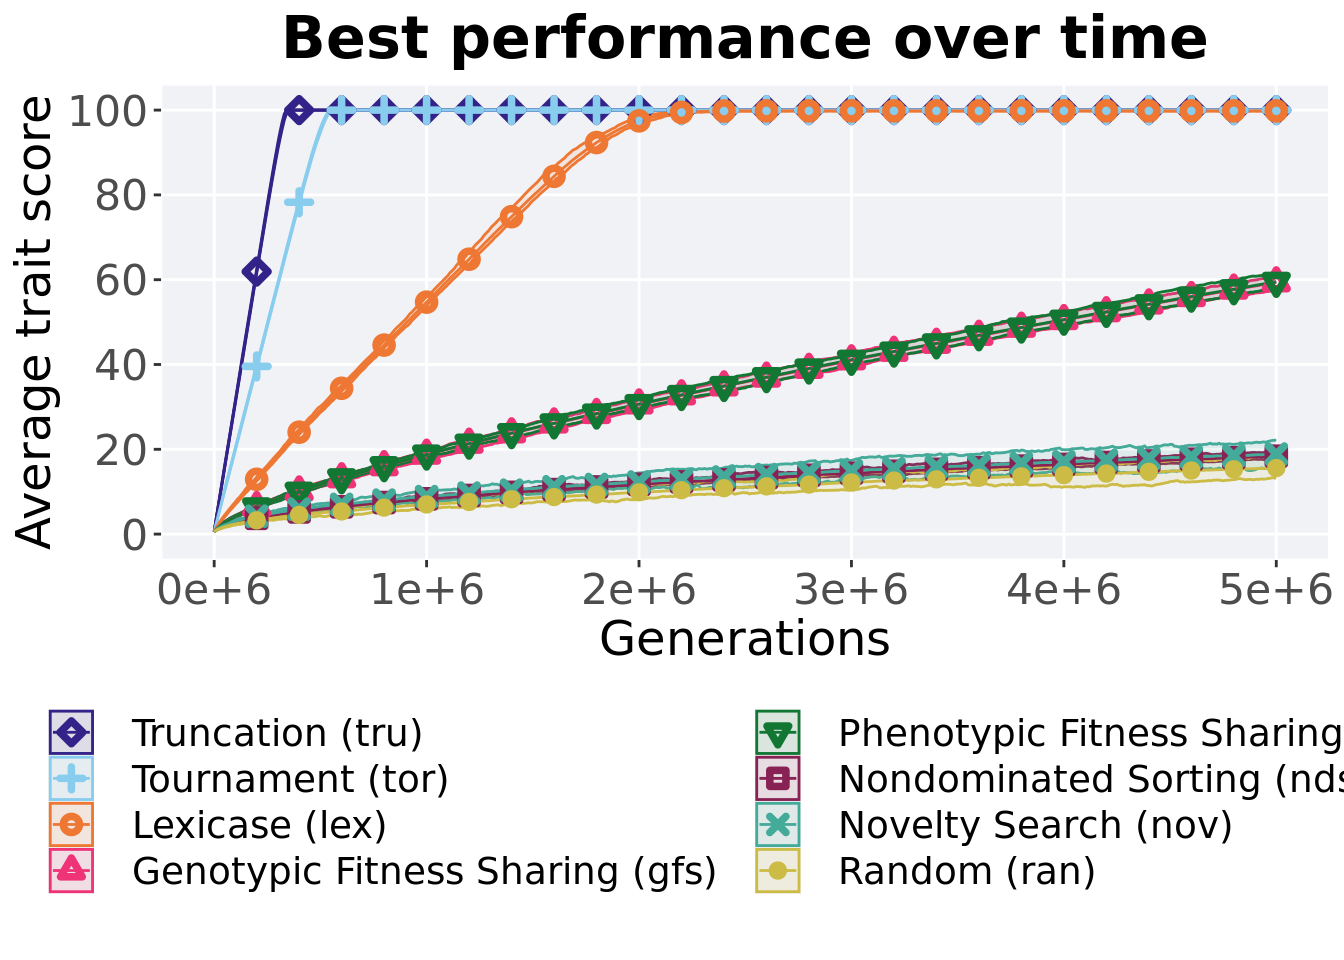
\includegraphics{demo_files/figure-latex/exp-per-ot-1.pdf}

\hypertarget{best-performance-throughout}{%
\section{Best performance throughout}\label{best-performance-throughout}}

Best performance found throughout 50,000 generations.

\begin{Shaded}
\begin{Highlighting}[]
\CommentTok{### best performance throughout}
\KeywordTok{filter}\NormalTok{(cc_best, col }\OperatorTok{==}\StringTok{ 'pop_fit_max'} \OperatorTok{&}\StringTok{ }\NormalTok{diagnostic }\OperatorTok{==}\StringTok{ 'exploitation_rate'}\NormalTok{) }\OperatorTok
\StringTok{  }\KeywordTok{ggplot}\NormalTok{(., }\KeywordTok{aes}\NormalTok{(}\DataTypeTok{x =}\NormalTok{ acron, }\DataTypeTok{y =}\NormalTok{ val }\OperatorTok{/}\StringTok{ }\NormalTok{DIMENSIONALITY, }\DataTypeTok{color =}\NormalTok{ acron, }\DataTypeTok{fill =}\NormalTok{ acron, }\DataTypeTok{shape =}\NormalTok{ acron)) }\OperatorTok{+}
\StringTok{  }\KeywordTok{geom_flat_violin}\NormalTok{(}\DataTypeTok{position =} \KeywordTok{position_nudge}\NormalTok{(}\DataTypeTok{x =} \FloatTok{.2}\NormalTok{, }\DataTypeTok{y =} \DecValTok{0}\NormalTok{), }\DataTypeTok{scale =} \StringTok{'width'}\NormalTok{, }\DataTypeTok{alpha =} \FloatTok{0.2}\NormalTok{) }\OperatorTok{+}
\StringTok{  }\KeywordTok{geom_point}\NormalTok{(}\DataTypeTok{position =} \KeywordTok{position_jitter}\NormalTok{(}\DataTypeTok{width =} \FloatTok{.1}\NormalTok{), }\DataTypeTok{size =} \FloatTok{1.5}\NormalTok{, }\DataTypeTok{alpha =} \FloatTok{1.0}\NormalTok{) }\OperatorTok{+}
\StringTok{  }\KeywordTok{geom_boxplot}\NormalTok{(}\DataTypeTok{color =} \StringTok{'black'}\NormalTok{, }\DataTypeTok{width =} \FloatTok{.2}\NormalTok{, }\DataTypeTok{outlier.shape =} \OtherTok{NA}\NormalTok{, }\DataTypeTok{alpha =} \FloatTok{0.0}\NormalTok{) }\OperatorTok{+}
\StringTok{  }\KeywordTok{scale_y_continuous}\NormalTok{(}
    \DataTypeTok{name=}\StringTok{"Average trait score"}\NormalTok{,}
    \DataTypeTok{limits=}\KeywordTok{c}\NormalTok{(}\OperatorTok{-}\DecValTok{1}\NormalTok{, }\DecValTok{101}\NormalTok{),}
    \DataTypeTok{breaks=}\KeywordTok{seq}\NormalTok{(}\DecValTok{0}\NormalTok{,}\DecValTok{100}\NormalTok{, }\DecValTok{20}\NormalTok{),}
    \DataTypeTok{labels=}\KeywordTok{c}\NormalTok{(}\StringTok{"0"}\NormalTok{, }\StringTok{"20"}\NormalTok{, }\StringTok{"40"}\NormalTok{, }\StringTok{"60"}\NormalTok{, }\StringTok{"80"}\NormalTok{, }\StringTok{"100"}\NormalTok{)}
\NormalTok{  ) }\OperatorTok{+}
\StringTok{  }\KeywordTok{scale_x_discrete}\NormalTok{(}
    \DataTypeTok{name=}\StringTok{"Scheme"}
\NormalTok{  )}\OperatorTok{+}
\StringTok{  }\KeywordTok{scale_shape_manual}\NormalTok{(}\DataTypeTok{values=}\NormalTok{SHAPE)}\OperatorTok{+}
\StringTok{  }\KeywordTok{scale_colour_manual}\NormalTok{(}\DataTypeTok{values =}\NormalTok{ cb_palette, ) }\OperatorTok{+}
\StringTok{  }\KeywordTok{scale_fill_manual}\NormalTok{(}\DataTypeTok{values =}\NormalTok{ cb_palette) }\OperatorTok{+}
\StringTok{  }\KeywordTok{ggtitle}\NormalTok{(}\StringTok{'Best performance throughout'}\NormalTok{)}\OperatorTok{+}
\StringTok{  }\NormalTok{p_theme }\OperatorTok{+}\StringTok{ }\KeywordTok{theme}\NormalTok{(}\DataTypeTok{legend.title=}\KeywordTok{element_blank}\NormalTok{()) }\OperatorTok{+}
\StringTok{  }\KeywordTok{guides}\NormalTok{(}
    \DataTypeTok{shape=}\KeywordTok{guide_legend}\NormalTok{(}\DataTypeTok{nrow=}\DecValTok{2}\NormalTok{, }\DataTypeTok{title.position =} \StringTok{"bottom"}\NormalTok{),}
    \DataTypeTok{color=}\KeywordTok{guide_legend}\NormalTok{(}\DataTypeTok{nrow=}\DecValTok{2}\NormalTok{, }\DataTypeTok{title.position =} \StringTok{"bottom"}\NormalTok{),}
    \DataTypeTok{fill=}\KeywordTok{guide_legend}\NormalTok{(}\DataTypeTok{nrow=}\DecValTok{2}\NormalTok{, }\DataTypeTok{title.position =} \StringTok{"bottom"}\NormalTok{)}
\NormalTok{  )}
\end{Highlighting}
\end{Shaded}

\begin{verbatim}
## Warning: Using the `size` aesthietic with geom_polygon was deprecated in ggplot2 3.4.0.
## i Please use the `linewidth` aesthetic instead.
\end{verbatim}

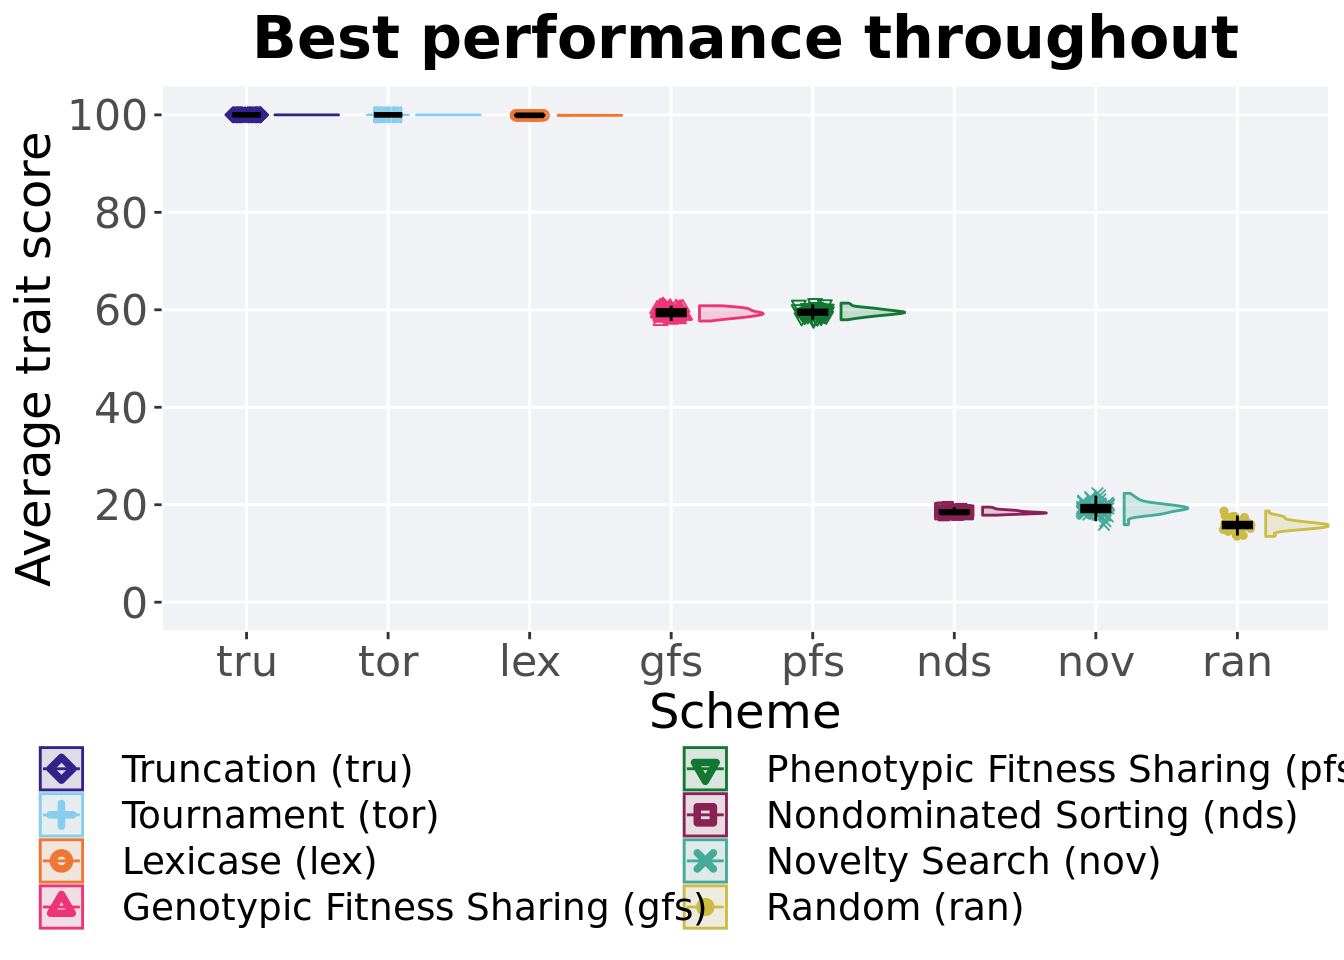
\includegraphics{demo_files/figure-latex/exp-per-bst-1.pdf}

\hypertarget{stats}{%
\subsection{Stats}\label{stats}}

Summary statistics for the best performance.

\begin{Shaded}
\begin{Highlighting}[]
\CommentTok{#get data & summarize}
\NormalTok{performance =}\StringTok{ }\KeywordTok{filter}\NormalTok{(cc_best, col }\OperatorTok{==}\StringTok{ 'pop_fit_max'} \OperatorTok{&}\StringTok{ }\NormalTok{diagnostic }\OperatorTok{==}\StringTok{ 'exploitation_rate'}\NormalTok{)}
\NormalTok{performance}\OperatorTok{$}\NormalTok{acron =}\StringTok{ }\KeywordTok{factor}\NormalTok{(performance}\OperatorTok{$}\NormalTok{acron, }\DataTypeTok{levels =} \KeywordTok{c}\NormalTok{(}\StringTok{'tru'}\NormalTok{, }\StringTok{'tor'}\NormalTok{, }\StringTok{'lex'}\NormalTok{, }\StringTok{'gfs'}\NormalTok{, }\StringTok{'pfs'}\NormalTok{, }\StringTok{'nov'}\NormalTok{, }\StringTok{'nds'}\NormalTok{, }\StringTok{'ran'}\NormalTok{))}
\NormalTok{performance }\OperatorTok
\StringTok{  }\KeywordTok{group_by}\NormalTok{(acron) }\OperatorTok
\StringTok{  }\NormalTok{dplyr}\OperatorTok{::}\KeywordTok{summarise}\NormalTok{(}
    \DataTypeTok{count =} \KeywordTok{n}\NormalTok{(),}
    \DataTypeTok{na_cnt =} \KeywordTok{sum}\NormalTok{(}\KeywordTok{is.na}\NormalTok{(val)),}
    \DataTypeTok{min =} \KeywordTok{min}\NormalTok{(val }\OperatorTok{/}\StringTok{ }\NormalTok{DIMENSIONALITY, }\DataTypeTok{na.rm =} \OtherTok{TRUE}\NormalTok{),}
    \DataTypeTok{median =} \KeywordTok{median}\NormalTok{(val }\OperatorTok{/}\StringTok{ }\NormalTok{DIMENSIONALITY, }\DataTypeTok{na.rm =} \OtherTok{TRUE}\NormalTok{),}
    \DataTypeTok{mean =} \KeywordTok{mean}\NormalTok{(val }\OperatorTok{/}\StringTok{ }\NormalTok{DIMENSIONALITY, }\DataTypeTok{na.rm =} \OtherTok{TRUE}\NormalTok{),}
    \DataTypeTok{max =} \KeywordTok{max}\NormalTok{(val }\OperatorTok{/}\StringTok{ }\NormalTok{DIMENSIONALITY, }\DataTypeTok{na.rm =} \OtherTok{TRUE}\NormalTok{),}
    \DataTypeTok{IQR =} \KeywordTok{IQR}\NormalTok{(val }\OperatorTok{/}\StringTok{ }\NormalTok{DIMENSIONALITY, }\DataTypeTok{na.rm =} \OtherTok{TRUE}\NormalTok{)}
\NormalTok{  )}
\end{Highlighting}
\end{Shaded}

\begin{verbatim}
## # A tibble: 8 x 8
##   acron count na_cnt   min median  mean   max    IQR
##   <fct> <int>  <int> <dbl>  <dbl> <dbl> <dbl>  <dbl>
## 1 tru      50      0 100    100   100   100   0     
## 2 tor      50      0 100    100   100   100   0     
## 3 lex      50      0  99.9   99.9  99.9  99.9 0.0137
## 4 gfs      50      0  57.7   59.3  59.4  60.8 1.31  
## 5 pfs      50      0  58.0   59.5  59.5  61.4 0.908 
## 6 nov      50      0  15.9   19.2  19.3  22.3 1.34  
## 7 nds      50      0  17.9   18.4  18.5  19.5 0.516 
## 8 ran      50      0  13.5   15.9  15.9  18.7 1.15
\end{verbatim}

Kruskal--Wallis test provides evidence of statistical differences.

\begin{Shaded}
\begin{Highlighting}[]
\KeywordTok{kruskal.test}\NormalTok{(val }\OperatorTok{~}\StringTok{ }\NormalTok{acron, }\DataTypeTok{data =}\NormalTok{ performance)}
\end{Highlighting}
\end{Shaded}

\begin{verbatim}
## 
##  Kruskal-Wallis rank sum test
## 
## data:  val by acron
## Kruskal-Wallis chi-squared = 384.91, df = 7, p-value < 2.2e-16
\end{verbatim}

Results for post-hoc Wilcoxon rank-sum test with a Bonferroni correction.

\begin{Shaded}
\begin{Highlighting}[]
\KeywordTok{pairwise.wilcox.test}\NormalTok{(}\DataTypeTok{x =}\NormalTok{ performance}\OperatorTok{$}\NormalTok{val, }\DataTypeTok{g =}\NormalTok{ performance}\OperatorTok{$}\NormalTok{acron, }\DataTypeTok{p.adjust.method =} \StringTok{"bonferroni"}\NormalTok{,}
                     \DataTypeTok{paired =} \OtherTok{FALSE}\NormalTok{, }\DataTypeTok{conf.int =} \OtherTok{FALSE}\NormalTok{, }\DataTypeTok{alternative =} \StringTok{'l'}\NormalTok{)}
\end{Highlighting}
\end{Shaded}

\begin{verbatim}
## 
##  Pairwise comparisons using Wilcoxon rank sum test with continuity correction 
## 
## data:  performance$val and performance$acron 
## 
##     tru     tor     lex     gfs     pfs     nov     nds    
## tor 1e+00   -       -       -       -       -       -      
## lex < 2e-16 < 2e-16 -       -       -       -       -      
## gfs < 2e-16 < 2e-16 < 2e-16 -       -       -       -      
## pfs < 2e-16 < 2e-16 < 2e-16 1e+00   -       -       -      
## nov < 2e-16 < 2e-16 < 2e-16 < 2e-16 < 2e-16 -       -      
## nds < 2e-16 < 2e-16 < 2e-16 < 2e-16 < 2e-16 6e-04   -      
## ran < 2e-16 < 2e-16 < 2e-16 < 2e-16 < 2e-16 1.9e-15 7.9e-16
## 
## P value adjustment method: bonferroni
\end{verbatim}

\hypertarget{generation-satisfactory-solution-found}{%
\section{Generation satisfactory solution found}\label{generation-satisfactory-solution-found}}

First generation a satisfactory solution is found throughout the 50,000 generations.

\begin{Shaded}
\begin{Highlighting}[]
\KeywordTok{filter}\NormalTok{(cc_ssf, diagnostic }\OperatorTok{==}\StringTok{ 'exploitation_rate'}\NormalTok{) }\OperatorTok
\StringTok{  }\KeywordTok{ggplot}\NormalTok{(., }\KeywordTok{aes}\NormalTok{(}\DataTypeTok{x =}\NormalTok{ acron, }\DataTypeTok{y =}\NormalTok{ Generations , }\DataTypeTok{color =}\NormalTok{ acron, }\DataTypeTok{fill =}\NormalTok{ acron, }\DataTypeTok{shape =}\NormalTok{ acron)) }\OperatorTok{+}
\StringTok{  }\KeywordTok{geom_flat_violin}\NormalTok{(}\DataTypeTok{position =} \KeywordTok{position_nudge}\NormalTok{(}\DataTypeTok{x =} \FloatTok{.2}\NormalTok{, }\DataTypeTok{y =} \DecValTok{0}\NormalTok{), }\DataTypeTok{scale =} \StringTok{'width'}\NormalTok{, }\DataTypeTok{alpha =} \FloatTok{0.2}\NormalTok{) }\OperatorTok{+}
\StringTok{  }\KeywordTok{geom_point}\NormalTok{(}\DataTypeTok{position =} \KeywordTok{position_jitter}\NormalTok{(}\DataTypeTok{width =} \FloatTok{.1}\NormalTok{), }\DataTypeTok{size =} \FloatTok{1.5}\NormalTok{, }\DataTypeTok{alpha =} \FloatTok{1.0}\NormalTok{) }\OperatorTok{+}
\StringTok{  }\KeywordTok{geom_boxplot}\NormalTok{(}\DataTypeTok{color =} \StringTok{'black'}\NormalTok{, }\DataTypeTok{width =} \FloatTok{.2}\NormalTok{, }\DataTypeTok{outlier.shape =} \OtherTok{NA}\NormalTok{, }\DataTypeTok{alpha =} \FloatTok{0.0}\NormalTok{) }\OperatorTok{+}
\StringTok{  }\KeywordTok{scale_y_continuous}\NormalTok{(}
    \DataTypeTok{name=}\StringTok{"Generation"}\NormalTok{,}
    \DataTypeTok{limits=}\KeywordTok{c}\NormalTok{(}\DecValTok{0}\NormalTok{, }\DecValTok{60001}\NormalTok{),}
    \DataTypeTok{breaks=}\KeywordTok{c}\NormalTok{(}\DecValTok{0}\NormalTok{, }\DecValTok{10000}\NormalTok{, }\DecValTok{20000}\NormalTok{, }\DecValTok{30000}\NormalTok{, }\DecValTok{40000}\NormalTok{, }\DecValTok{50000}\NormalTok{, }\DecValTok{60000}\NormalTok{),}
    \DataTypeTok{labels=}\KeywordTok{c}\NormalTok{(}\StringTok{"0e+4"}\NormalTok{, }\StringTok{"1e+4"}\NormalTok{, }\StringTok{"2e+4"}\NormalTok{, }\StringTok{"3e+4"}\NormalTok{, }\StringTok{"4e+4"}\NormalTok{, }\StringTok{"5e+4"}\NormalTok{, }\StringTok{"Fail"}\NormalTok{)}
\NormalTok{  ) }\OperatorTok{+}
\StringTok{  }\KeywordTok{scale_x_discrete}\NormalTok{(}
    \DataTypeTok{name=}\StringTok{"Scheme"}
\NormalTok{  )}\OperatorTok{+}
\StringTok{  }\KeywordTok{scale_shape_manual}\NormalTok{(}\DataTypeTok{values=}\NormalTok{SHAPE)}\OperatorTok{+}
\StringTok{  }\KeywordTok{scale_colour_manual}\NormalTok{(}\DataTypeTok{values =}\NormalTok{ cb_palette, ) }\OperatorTok{+}
\StringTok{  }\KeywordTok{scale_fill_manual}\NormalTok{(}\DataTypeTok{values =}\NormalTok{ cb_palette) }\OperatorTok{+}
\StringTok{  }\KeywordTok{ggtitle}\NormalTok{(}\StringTok{'Generation satisfactory solution found'}\NormalTok{)}\OperatorTok{+}
\StringTok{  }\NormalTok{p_theme }\OperatorTok{+}\StringTok{ }\KeywordTok{theme}\NormalTok{(}\DataTypeTok{legend.title=}\KeywordTok{element_blank}\NormalTok{()) }\OperatorTok{+}
\StringTok{  }\KeywordTok{guides}\NormalTok{(}
    \DataTypeTok{shape=}\KeywordTok{guide_legend}\NormalTok{(}\DataTypeTok{nrow=}\DecValTok{2}\NormalTok{, }\DataTypeTok{title.position =} \StringTok{"bottom"}\NormalTok{),}
    \DataTypeTok{color=}\KeywordTok{guide_legend}\NormalTok{(}\DataTypeTok{nrow=}\DecValTok{2}\NormalTok{, }\DataTypeTok{title.position =} \StringTok{"bottom"}\NormalTok{),}
    \DataTypeTok{fill=}\KeywordTok{guide_legend}\NormalTok{(}\DataTypeTok{nrow=}\DecValTok{2}\NormalTok{, }\DataTypeTok{title.position =} \StringTok{"bottom"}\NormalTok{)}
\NormalTok{  )}
\end{Highlighting}
\end{Shaded}

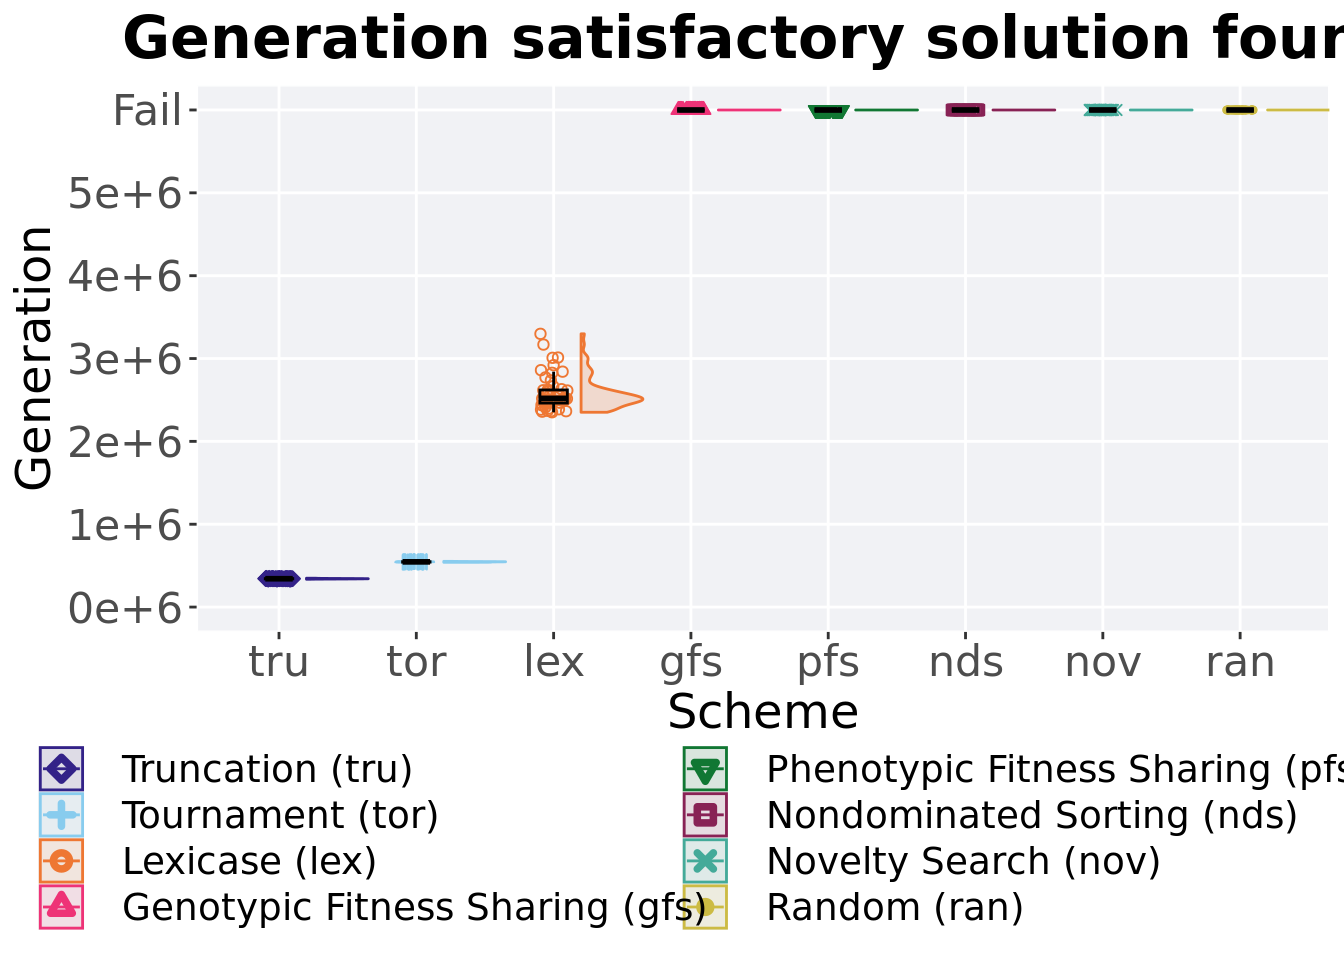
\includegraphics{demo_files/figure-latex/exp-ssf-1.pdf}

\hypertarget{stats-1}{%
\subsection{Stats}\label{stats-1}}

Summary statistics for the first generation a satisfactory solution is found.

\begin{Shaded}
\begin{Highlighting}[]
\NormalTok{ssf =}\StringTok{ }\KeywordTok{filter}\NormalTok{(cc_ssf, diagnostic }\OperatorTok{==}\StringTok{ 'exploitation_rate'}  \OperatorTok{&}\StringTok{ }\NormalTok{Generations }\OperatorTok{<}\StringTok{ }\DecValTok{60000}\NormalTok{)}
\NormalTok{ssf}\OperatorTok{$}\NormalTok{acron =}\StringTok{ }\KeywordTok{factor}\NormalTok{(ssf}\OperatorTok{$}\NormalTok{acron, }\DataTypeTok{levels =} \KeywordTok{c}\NormalTok{(}\StringTok{'tru'}\NormalTok{, }\StringTok{'tor'}\NormalTok{, }\StringTok{'lex'}\NormalTok{))}
\NormalTok{ssf }\OperatorTok
\StringTok{  }\KeywordTok{group_by}\NormalTok{(acron) }\OperatorTok
\StringTok{  }\NormalTok{dplyr}\OperatorTok{::}\KeywordTok{summarise}\NormalTok{(}
    \DataTypeTok{count =} \KeywordTok{n}\NormalTok{(),}
    \DataTypeTok{na_cnt =} \KeywordTok{sum}\NormalTok{(}\KeywordTok{is.na}\NormalTok{(Generations)),}
    \DataTypeTok{min =} \KeywordTok{min}\NormalTok{(Generations, }\DataTypeTok{na.rm =} \OtherTok{TRUE}\NormalTok{),}
    \DataTypeTok{median =} \KeywordTok{median}\NormalTok{(Generations, }\DataTypeTok{na.rm =} \OtherTok{TRUE}\NormalTok{),}
    \DataTypeTok{mean =} \KeywordTok{mean}\NormalTok{(Generations, }\DataTypeTok{na.rm =} \OtherTok{TRUE}\NormalTok{),}
    \DataTypeTok{max =} \KeywordTok{max}\NormalTok{(Generations, }\DataTypeTok{na.rm =} \OtherTok{TRUE}\NormalTok{),}
    \DataTypeTok{IQR =} \KeywordTok{IQR}\NormalTok{(Generations, }\DataTypeTok{na.rm =} \OtherTok{TRUE}\NormalTok{)}
\NormalTok{  )}
\end{Highlighting}
\end{Shaded}

\begin{verbatim}
## # A tibble: 3 x 8
##   acron count na_cnt   min median   mean   max    IQR
##   <fct> <int>  <int> <int>  <dbl>  <dbl> <int>  <dbl>
## 1 tru      50      0  3357   3420  3421.  3481   34.2
## 2 tor      50      0  5403   5457  5453.  5519   51.8
## 3 lex      50      0 23514  25190 25857. 32980 1581
\end{verbatim}

Kruskal--Wallis test provides evidence of difference amoung selection schemes.

\begin{Shaded}
\begin{Highlighting}[]
\KeywordTok{kruskal.test}\NormalTok{(Generations }\OperatorTok{~}\StringTok{ }\NormalTok{acron, }\DataTypeTok{data =}\NormalTok{ ssf)}
\end{Highlighting}
\end{Shaded}

\begin{verbatim}
## 
##  Kruskal-Wallis rank sum test
## 
## data:  Generations by acron
## Kruskal-Wallis chi-squared = 132.46, df = 2, p-value < 2.2e-16
\end{verbatim}

Results for post-hoc Wilcoxon rank-sum test with a Bonferroni correction.

\begin{Shaded}
\begin{Highlighting}[]
\KeywordTok{pairwise.wilcox.test}\NormalTok{(}\DataTypeTok{x =}\NormalTok{ ssf}\OperatorTok{$}\NormalTok{Generations, }\DataTypeTok{g =}\NormalTok{ ssf}\OperatorTok{$}\NormalTok{acron, }\DataTypeTok{p.adjust.method =} \StringTok{"bonferroni"}\NormalTok{,}
                     \DataTypeTok{paired =} \OtherTok{FALSE}\NormalTok{, }\DataTypeTok{conf.int =} \OtherTok{FALSE}\NormalTok{, }\DataTypeTok{alternative =} \StringTok{'g'}\NormalTok{)}
\end{Highlighting}
\end{Shaded}

\begin{verbatim}
## 
##  Pairwise comparisons using Wilcoxon rank sum test with continuity correction 
## 
## data:  ssf$Generations and ssf$acron 
## 
##     tru    tor   
## tor <2e-16 -     
## lex <2e-16 <2e-16
## 
## P value adjustment method: bonferroni
\end{verbatim}

\hypertarget{multi-valley-crossing-results}{%
\section{Multi-valley crossing results}\label{multi-valley-crossing-results}}

\hypertarget{performance-over-time-1}{%
\subsection{Performance over time}\label{performance-over-time-1}}

Best performance in a population over time.

\begin{Shaded}
\begin{Highlighting}[]
\CommentTok{# data for lines and shading on plots}
\NormalTok{lines =}\StringTok{ }\KeywordTok{filter}\NormalTok{(cc_over_time_mvc, diagnostic }\OperatorTok{==}\StringTok{ 'exploitation_rate'}\NormalTok{) }\OperatorTok
\StringTok{  }\KeywordTok{group_by}\NormalTok{(}\StringTok{`}\DataTypeTok{Selection}\CharTok{\textbackslash{}n}\DataTypeTok{Scheme}\StringTok{`}\NormalTok{, gen) }\OperatorTok
\StringTok{  }\NormalTok{dplyr}\OperatorTok{::}\KeywordTok{summarise}\NormalTok{(}
    \DataTypeTok{min =} \KeywordTok{min}\NormalTok{(pop_fit_max) }\OperatorTok{/}\StringTok{ }\NormalTok{DIMENSIONALITY,}
    \DataTypeTok{mean =} \KeywordTok{mean}\NormalTok{(pop_fit_max) }\OperatorTok{/}\StringTok{ }\NormalTok{DIMENSIONALITY,}
    \DataTypeTok{max =} \KeywordTok{max}\NormalTok{(pop_fit_max) }\OperatorTok{/}\StringTok{ }\NormalTok{DIMENSIONALITY}
\NormalTok{  )}
\end{Highlighting}
\end{Shaded}

\begin{verbatim}
## `summarise()` has grouped output by 'Selection Scheme'. You can override using
## the `.groups` argument.
\end{verbatim}

\begin{Shaded}
\begin{Highlighting}[]
\KeywordTok{ggplot}\NormalTok{(lines, }\KeywordTok{aes}\NormalTok{(}\DataTypeTok{x=}\NormalTok{gen, }\DataTypeTok{y=}\NormalTok{mean, }\DataTypeTok{group =} \StringTok{`}\DataTypeTok{Selection}\CharTok{\textbackslash{}n}\DataTypeTok{Scheme}\StringTok{`}\NormalTok{, }\DataTypeTok{fill =}\StringTok{`}\DataTypeTok{Selection}\CharTok{\textbackslash{}n}\DataTypeTok{Scheme}\StringTok{`}\NormalTok{, }\DataTypeTok{color =} \StringTok{`}\DataTypeTok{Selection}\CharTok{\textbackslash{}n}\DataTypeTok{Scheme}\StringTok{`}\NormalTok{, }\DataTypeTok{shape =} \StringTok{`}\DataTypeTok{Selection}\CharTok{\textbackslash{}n}\DataTypeTok{Scheme}\StringTok{`}\NormalTok{)) }\OperatorTok{+}
\StringTok{  }\KeywordTok{geom_ribbon}\NormalTok{(}\KeywordTok{aes}\NormalTok{(}\DataTypeTok{ymin =}\NormalTok{ min, }\DataTypeTok{ymax =}\NormalTok{ max), }\DataTypeTok{alpha =} \FloatTok{0.1}\NormalTok{) }\OperatorTok{+}
\StringTok{  }\KeywordTok{geom_line}\NormalTok{(}\DataTypeTok{size =} \FloatTok{0.5}\NormalTok{) }\OperatorTok{+}
\StringTok{  }\KeywordTok{geom_point}\NormalTok{(}\DataTypeTok{data =} \KeywordTok{filter}\NormalTok{(lines, gen }\OperatorTok\StringTok{ }\DecValTok{2000} \OperatorTok{==}\StringTok{ }\DecValTok{0} \OperatorTok{&}\StringTok{ }\NormalTok{gen }\OperatorTok{!=}\StringTok{ }\DecValTok{0}\NormalTok{), }\DataTypeTok{size =} \FloatTok{1.5}\NormalTok{, }\DataTypeTok{stroke =} \FloatTok{2.0}\NormalTok{, }\DataTypeTok{alpha =} \FloatTok{1.0}\NormalTok{) }\OperatorTok{+}
\StringTok{  }\KeywordTok{scale_y_continuous}\NormalTok{(}
    \DataTypeTok{name=}\StringTok{"Average trait score"}\NormalTok{,}
    \DataTypeTok{limits=}\KeywordTok{c}\NormalTok{(}\DecValTok{0}\NormalTok{, }\DecValTok{50}\NormalTok{),}
    \DataTypeTok{breaks=}\KeywordTok{seq}\NormalTok{(}\DecValTok{0}\NormalTok{,}\DecValTok{50}\NormalTok{, }\DecValTok{10}\NormalTok{),}
    \DataTypeTok{labels=}\KeywordTok{c}\NormalTok{(}\StringTok{"0"}\NormalTok{, }\StringTok{"10"}\NormalTok{, }\StringTok{"20"}\NormalTok{, }\StringTok{"30"}\NormalTok{, }\StringTok{"40"}\NormalTok{, }\StringTok{"50"}\NormalTok{)}
\NormalTok{  ) }\OperatorTok{+}
\StringTok{  }\KeywordTok{scale_x_continuous}\NormalTok{(}
    \DataTypeTok{name=}\StringTok{"Generations"}\NormalTok{,}
    \DataTypeTok{limits=}\KeywordTok{c}\NormalTok{(}\DecValTok{0}\NormalTok{, }\DecValTok{50000}\NormalTok{),}
    \DataTypeTok{breaks=}\KeywordTok{c}\NormalTok{(}\DecValTok{0}\NormalTok{, }\DecValTok{10000}\NormalTok{, }\DecValTok{20000}\NormalTok{, }\DecValTok{30000}\NormalTok{, }\DecValTok{40000}\NormalTok{, }\DecValTok{50000}\NormalTok{),}
    \DataTypeTok{labels=}\KeywordTok{c}\NormalTok{(}\StringTok{"0e+4"}\NormalTok{, }\StringTok{"1e+4"}\NormalTok{, }\StringTok{"2e+4"}\NormalTok{, }\StringTok{"3e+4"}\NormalTok{, }\StringTok{"4e+4"}\NormalTok{, }\StringTok{"5e+4"}\NormalTok{)}

\NormalTok{  ) }\OperatorTok{+}
\StringTok{  }\KeywordTok{scale_shape_manual}\NormalTok{(}\DataTypeTok{values=}\NormalTok{SHAPE)}\OperatorTok{+}
\StringTok{  }\KeywordTok{scale_colour_manual}\NormalTok{(}\DataTypeTok{values =}\NormalTok{ cb_palette) }\OperatorTok{+}
\StringTok{  }\KeywordTok{scale_fill_manual}\NormalTok{(}\DataTypeTok{values =}\NormalTok{ cb_palette) }\OperatorTok{+}
\StringTok{  }\KeywordTok{ggtitle}\NormalTok{(}\StringTok{'Performance over time'}\NormalTok{)}\OperatorTok{+}
\StringTok{  }\NormalTok{p_theme }\OperatorTok{+}\StringTok{ }\KeywordTok{theme}\NormalTok{(}\DataTypeTok{legend.title=}\KeywordTok{element_blank}\NormalTok{(),}\DataTypeTok{legend.text=}\KeywordTok{element_text}\NormalTok{(}\DataTypeTok{size=}\DecValTok{12}\NormalTok{)) }\OperatorTok{+}
\StringTok{  }\KeywordTok{guides}\NormalTok{(}
    \DataTypeTok{sh=}\KeywordTok{guide_legend}\NormalTok{(}\DataTypeTok{ncol=}\DecValTok{2}\NormalTok{, }\DataTypeTok{title.position =} \StringTok{"left"}\NormalTok{),}
    \DataTypeTok{color=}\KeywordTok{guide_legend}\NormalTok{(}\DataTypeTok{ncol=}\DecValTok{2}\NormalTok{, }\DataTypeTok{title.position =} \StringTok{"left"}\NormalTok{),}
    \DataTypeTok{fillape=}\KeywordTok{guide_legend}\NormalTok{(}\DataTypeTok{ncol=}\DecValTok{2}\NormalTok{, }\DataTypeTok{title.position =} \StringTok{"left"}\NormalTok{)}
\NormalTok{  )}
\end{Highlighting}
\end{Shaded}

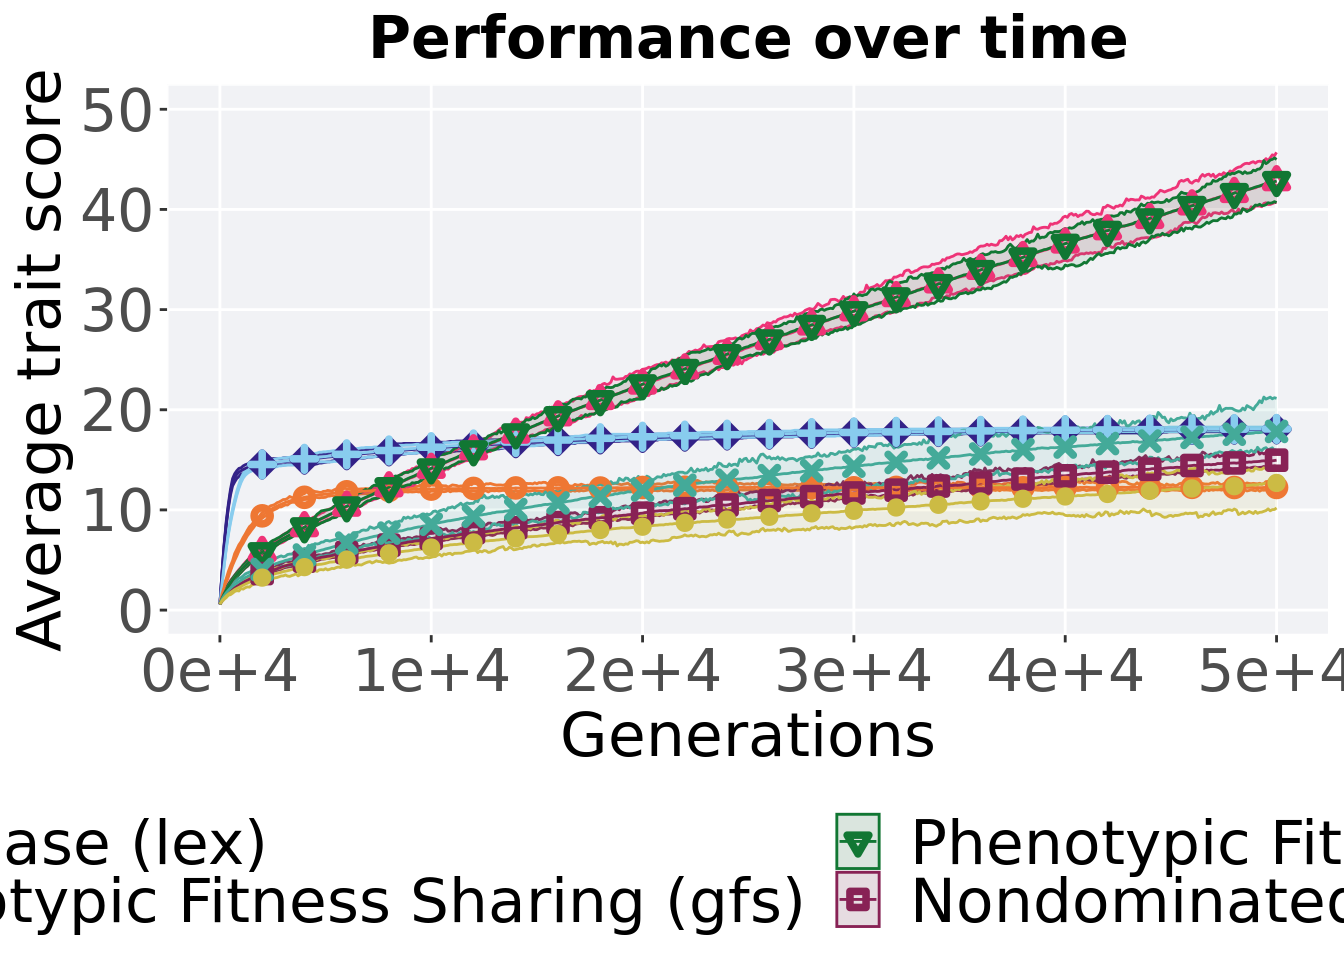
\includegraphics{demo_files/figure-latex/exp-mvc-per-ot-1.pdf}

\hypertarget{best-performance-throughout-1}{%
\subsection{Best performance throughout}\label{best-performance-throughout-1}}

Best performance found throughout 50,000 generations.

\begin{Shaded}
\begin{Highlighting}[]
\CommentTok{### best performance throughout}
\KeywordTok{filter}\NormalTok{(cc_best_mvc, col }\OperatorTok{==}\StringTok{ 'pop_fit_max'} \OperatorTok{&}\StringTok{ }\NormalTok{diagnostic }\OperatorTok{==}\StringTok{ 'exploitation_rate'}\NormalTok{) }\OperatorTok
\StringTok{  }\KeywordTok{ggplot}\NormalTok{(., }\KeywordTok{aes}\NormalTok{(}\DataTypeTok{x =}\NormalTok{ acron, }\DataTypeTok{y =}\NormalTok{ val }\OperatorTok{/}\StringTok{ }\NormalTok{DIMENSIONALITY, }\DataTypeTok{color =}\NormalTok{ acron, }\DataTypeTok{fill =}\NormalTok{ acron, }\DataTypeTok{shape =}\NormalTok{ acron)) }\OperatorTok{+}
\StringTok{  }\KeywordTok{geom_flat_violin}\NormalTok{(}\DataTypeTok{position =} \KeywordTok{position_nudge}\NormalTok{(}\DataTypeTok{x =} \FloatTok{.2}\NormalTok{, }\DataTypeTok{y =} \DecValTok{0}\NormalTok{), }\DataTypeTok{scale =} \StringTok{'width'}\NormalTok{, }\DataTypeTok{alpha =} \FloatTok{0.2}\NormalTok{) }\OperatorTok{+}
\StringTok{  }\KeywordTok{geom_point}\NormalTok{(}\DataTypeTok{position =} \KeywordTok{position_jitter}\NormalTok{(}\DataTypeTok{width =} \FloatTok{.1}\NormalTok{), }\DataTypeTok{size =} \FloatTok{1.5}\NormalTok{, }\DataTypeTok{alpha =} \FloatTok{1.0}\NormalTok{) }\OperatorTok{+}
\StringTok{  }\KeywordTok{geom_boxplot}\NormalTok{(}\DataTypeTok{color =} \StringTok{'black'}\NormalTok{, }\DataTypeTok{width =} \FloatTok{.2}\NormalTok{, }\DataTypeTok{outlier.shape =} \OtherTok{NA}\NormalTok{, }\DataTypeTok{alpha =} \FloatTok{0.0}\NormalTok{) }\OperatorTok{+}
\StringTok{  }\KeywordTok{scale_y_continuous}\NormalTok{(}
    \DataTypeTok{name=}\StringTok{"Average trait score"}\NormalTok{,}
    \DataTypeTok{limits=}\KeywordTok{c}\NormalTok{(}\DecValTok{0}\NormalTok{, }\DecValTok{50}\NormalTok{),}
    \DataTypeTok{breaks=}\KeywordTok{seq}\NormalTok{(}\DecValTok{0}\NormalTok{,}\DecValTok{50}\NormalTok{, }\DecValTok{10}\NormalTok{),}
    \DataTypeTok{labels=}\KeywordTok{c}\NormalTok{(}\StringTok{"0"}\NormalTok{, }\StringTok{"10"}\NormalTok{, }\StringTok{"20"}\NormalTok{, }\StringTok{"30"}\NormalTok{, }\StringTok{"40"}\NormalTok{, }\StringTok{"50"}\NormalTok{)}
\NormalTok{  ) }\OperatorTok{+}
\StringTok{  }\KeywordTok{scale_x_discrete}\NormalTok{(}
    \DataTypeTok{name=}\StringTok{"Scheme"}
\NormalTok{  )}\OperatorTok{+}
\StringTok{  }\KeywordTok{scale_shape_manual}\NormalTok{(}\DataTypeTok{values=}\NormalTok{SHAPE)}\OperatorTok{+}
\StringTok{  }\KeywordTok{scale_colour_manual}\NormalTok{(}\DataTypeTok{values =}\NormalTok{ cb_palette, ) }\OperatorTok{+}
\StringTok{  }\KeywordTok{scale_fill_manual}\NormalTok{(}\DataTypeTok{values =}\NormalTok{ cb_palette) }\OperatorTok{+}
\StringTok{  }\KeywordTok{ggtitle}\NormalTok{(}\StringTok{'Best performance throughout'}\NormalTok{)}\OperatorTok{+}
\StringTok{  }\NormalTok{p_theme }\OperatorTok{+}\StringTok{ }\KeywordTok{theme}\NormalTok{(}\DataTypeTok{legend.title=}\KeywordTok{element_blank}\NormalTok{()) }\OperatorTok{+}
\StringTok{  }\KeywordTok{guides}\NormalTok{(}
    \DataTypeTok{shape=}\KeywordTok{guide_legend}\NormalTok{(}\DataTypeTok{nrow=}\DecValTok{2}\NormalTok{, }\DataTypeTok{title.position =} \StringTok{"bottom"}\NormalTok{),}
    \DataTypeTok{color=}\KeywordTok{guide_legend}\NormalTok{(}\DataTypeTok{nrow=}\DecValTok{2}\NormalTok{, }\DataTypeTok{title.position =} \StringTok{"bottom"}\NormalTok{),}
    \DataTypeTok{fill=}\KeywordTok{guide_legend}\NormalTok{(}\DataTypeTok{nrow=}\DecValTok{2}\NormalTok{, }\DataTypeTok{title.position =} \StringTok{"bottom"}\NormalTok{)}
\NormalTok{  )}
\end{Highlighting}
\end{Shaded}

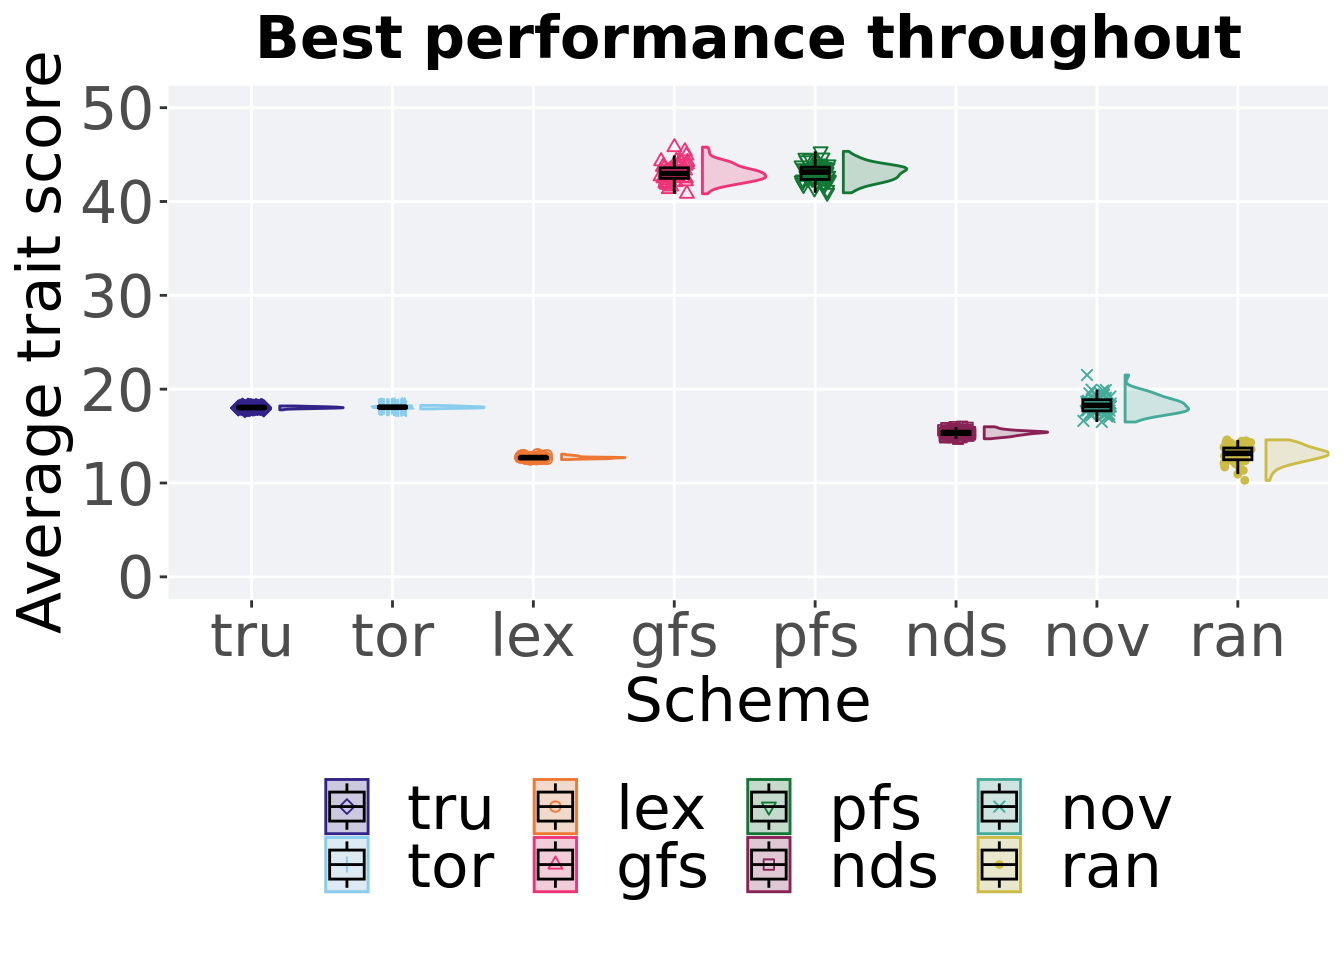
\includegraphics{demo_files/figure-latex/exp-mvc-per-bst-1.pdf}

\hypertarget{stats-2}{%
\subsubsection{Stats}\label{stats-2}}

Summary statistics for the performance of the best performance.

\begin{Shaded}
\begin{Highlighting}[]
\CommentTok{#get data & summarize}
\NormalTok{performance =}\StringTok{ }\KeywordTok{filter}\NormalTok{(cc_best_mvc, col }\OperatorTok{==}\StringTok{ 'pop_fit_max'} \OperatorTok{&}\StringTok{ }\NormalTok{diagnostic }\OperatorTok{==}\StringTok{ 'exploitation_rate'}\NormalTok{)}
\NormalTok{performance}\OperatorTok{$}\NormalTok{acron =}\StringTok{ }\KeywordTok{factor}\NormalTok{(performance}\OperatorTok{$}\NormalTok{acron, }\DataTypeTok{levels =} \KeywordTok{c}\NormalTok{(}\StringTok{'gfs'}\NormalTok{,}\StringTok{'pfs'}\NormalTok{,}\StringTok{'tru'}\NormalTok{,}\StringTok{'tor'}\NormalTok{,}\StringTok{'nov'}\NormalTok{, }\StringTok{'nds'}\NormalTok{,}\StringTok{'lex'}\NormalTok{, }\StringTok{'ran'}\NormalTok{))}
\NormalTok{performance }\OperatorTok
\StringTok{  }\KeywordTok{group_by}\NormalTok{(acron) }\OperatorTok
\StringTok{  }\NormalTok{dplyr}\OperatorTok{::}\KeywordTok{summarise}\NormalTok{(}
    \DataTypeTok{count =} \KeywordTok{n}\NormalTok{(),}
    \DataTypeTok{na_cnt =} \KeywordTok{sum}\NormalTok{(}\KeywordTok{is.na}\NormalTok{(val)),}
    \DataTypeTok{min =} \KeywordTok{min}\NormalTok{(val }\OperatorTok{/}\StringTok{ }\NormalTok{DIMENSIONALITY, }\DataTypeTok{na.rm =} \OtherTok{TRUE}\NormalTok{),}
    \DataTypeTok{median =} \KeywordTok{median}\NormalTok{(val }\OperatorTok{/}\StringTok{ }\NormalTok{DIMENSIONALITY, }\DataTypeTok{na.rm =} \OtherTok{TRUE}\NormalTok{),}
    \DataTypeTok{mean =} \KeywordTok{mean}\NormalTok{(val }\OperatorTok{/}\StringTok{ }\NormalTok{DIMENSIONALITY, }\DataTypeTok{na.rm =} \OtherTok{TRUE}\NormalTok{),}
    \DataTypeTok{max =} \KeywordTok{max}\NormalTok{(val }\OperatorTok{/}\StringTok{ }\NormalTok{DIMENSIONALITY, }\DataTypeTok{na.rm =} \OtherTok{TRUE}\NormalTok{),}
    \DataTypeTok{IQR =} \KeywordTok{IQR}\NormalTok{(val }\OperatorTok{/}\StringTok{ }\NormalTok{DIMENSIONALITY, }\DataTypeTok{na.rm =} \OtherTok{TRUE}\NormalTok{)}
\NormalTok{  )}
\end{Highlighting}
\end{Shaded}

\begin{verbatim}
## # A tibble: 8 x 8
##   acron count na_cnt   min median  mean   max   IQR
##   <fct> <int>  <int> <dbl>  <dbl> <dbl> <dbl> <dbl>
## 1 gfs      50      0  40.8   43.0  43.0  45.8 1.12 
## 2 pfs      50      0  40.9   43.1  43.1  45.3 1.30 
## 3 tru      50      0  17.8   18.0  18.0  18.2 0.118
## 4 tor      50      0  17.9   18.1  18.1  18.3 0.130
## 5 nov      50      0  16.5   18.3  18.3  21.5 1.19 
## 6 nds      50      0  14.7   15.4  15.3  16.0 0.318
## 7 lex      50      0  12.5   12.7  12.7  13.1 0.121
## 8 ran      50      0  10.3   13.2  13.1  14.6 1.25
\end{verbatim}

Kruskal--Wallis test provides evidence of statistical differences.

\begin{Shaded}
\begin{Highlighting}[]
\KeywordTok{kruskal.test}\NormalTok{(val }\OperatorTok{~}\StringTok{ }\NormalTok{acron, }\DataTypeTok{data =}\NormalTok{ performance)}
\end{Highlighting}
\end{Shaded}

\begin{verbatim}
## 
##  Kruskal-Wallis rank sum test
## 
## data:  val by acron
## Kruskal-Wallis chi-squared = 366.01, df = 7, p-value < 2.2e-16
\end{verbatim}

Results for post-hoc Wilcoxon rank-sum test with a Bonferroni correction.

\begin{Shaded}
\begin{Highlighting}[]
\KeywordTok{pairwise.wilcox.test}\NormalTok{(}\DataTypeTok{x =}\NormalTok{ performance}\OperatorTok{$}\NormalTok{val, }\DataTypeTok{g =}\NormalTok{ performance}\OperatorTok{$}\NormalTok{acron, }\DataTypeTok{p.adjust.method =} \StringTok{"bonferroni"}\NormalTok{,}
                     \DataTypeTok{paired =} \OtherTok{FALSE}\NormalTok{, }\DataTypeTok{conf.int =} \OtherTok{FALSE}\NormalTok{, }\DataTypeTok{alternative =} \StringTok{'l'}\NormalTok{)}
\end{Highlighting}
\end{Shaded}

\begin{verbatim}
## 
##  Pairwise comparisons using Wilcoxon rank sum test with continuity correction 
## 
## data:  performance$val and performance$acron 
## 
##     gfs    pfs    tru    tor    nov    nds    lex
## pfs 1      -      -      -      -      -      -  
## tru <2e-16 <2e-16 -      -      -      -      -  
## tor <2e-16 <2e-16 1      -      -      -      -  
## nov <2e-16 <2e-16 1      1      -      -      -  
## nds <2e-16 <2e-16 <2e-16 <2e-16 <2e-16 -      -  
## lex <2e-16 <2e-16 <2e-16 <2e-16 <2e-16 <2e-16 -  
## ran <2e-16 <2e-16 <2e-16 <2e-16 <2e-16 <2e-16 1  
## 
## P value adjustment method: bonferroni
\end{verbatim}

\hypertarget{performance-comparison}{%
\subsection{Performance comparison}\label{performance-comparison}}

Best performances in the population at 40,000 and 50,000 generations.

\begin{verbatim}
## Warning: The following aesthetics were dropped during statistical transformation:
## colour, shape
## i This can happen when ggplot fails to infer the correct grouping structure in
##   the data.
## i Did you forget to specify a `group` aesthetic or to convert a numerical
##   variable into a factor?
## The following aesthetics were dropped during statistical transformation:
## colour, shape
## i This can happen when ggplot fails to infer the correct grouping structure in
##   the data.
## i Did you forget to specify a `group` aesthetic or to convert a numerical
##   variable into a factor?
\end{verbatim}

\begin{Shaded}
\begin{Highlighting}[]
\CommentTok{# 80% and final generation comparison}
\NormalTok{end =}\StringTok{ }\KeywordTok{filter}\NormalTok{(cc_over_time_mvc, diagnostic }\OperatorTok{==}\StringTok{ 'exploitation_rate'} \OperatorTok{&}\StringTok{ }\NormalTok{gen }\OperatorTok{==}\StringTok{ }\DecValTok{50000} \OperatorTok{&}\StringTok{ }\NormalTok{acron }\OperatorTok{!=}\StringTok{ 'ran'}\NormalTok{)}
\NormalTok{end}\OperatorTok{$}\NormalTok{Generation <-}\StringTok{ }\KeywordTok{factor}\NormalTok{(end}\OperatorTok{$}\NormalTok{gen)}

\NormalTok{mid =}\StringTok{ }\KeywordTok{filter}\NormalTok{(cc_over_time_mvc, diagnostic }\OperatorTok{==}\StringTok{ 'exploitation_rate'} \OperatorTok{&}\StringTok{ }\NormalTok{gen }\OperatorTok{==}\StringTok{ }\DecValTok{40000} \OperatorTok{&}\StringTok{ }\NormalTok{acron }\OperatorTok{!=}\StringTok{ 'ran'}\NormalTok{)}
\NormalTok{mid}\OperatorTok{$}\NormalTok{Generation <-}\StringTok{ }\KeywordTok{factor}\NormalTok{(mid}\OperatorTok{$}\NormalTok{gen)}

\NormalTok{mvc_p =}\StringTok{ }\KeywordTok{ggplot}\NormalTok{(mid, }\KeywordTok{aes}\NormalTok{(}\DataTypeTok{x =}\NormalTok{ acron, }\DataTypeTok{y=}\NormalTok{pop_fit_max }\OperatorTok{/}\StringTok{ }\NormalTok{DIMENSIONALITY, }\DataTypeTok{group =}\NormalTok{ acron, }\DataTypeTok{shape =}\NormalTok{ Generation)) }\OperatorTok{+}
\StringTok{          }\KeywordTok{geom_point}\NormalTok{(}\DataTypeTok{col =}\NormalTok{ mvc_col[}\DecValTok{1}\NormalTok{] , }\DataTypeTok{position =} \KeywordTok{position_jitternudge}\NormalTok{(}\DataTypeTok{jitter.width =} \FloatTok{.03}\NormalTok{, }\DataTypeTok{nudge.x =} \FloatTok{-0.05}\NormalTok{), }\DataTypeTok{size =} \DecValTok{2}\NormalTok{, }\DataTypeTok{alpha =} \FloatTok{1.0}\NormalTok{) }\OperatorTok{+}
\StringTok{          }\KeywordTok{geom_boxplot}\NormalTok{(}\DataTypeTok{position =} \KeywordTok{position_nudge}\NormalTok{(}\DataTypeTok{x =} \FloatTok{-.15}\NormalTok{, }\DataTypeTok{y =} \DecValTok{0}\NormalTok{), }\DataTypeTok{lwd =} \FloatTok{0.7}\NormalTok{, }\DataTypeTok{col =}\NormalTok{ mvc_col[}\DecValTok{1}\NormalTok{], }\DataTypeTok{fill =}\NormalTok{ mvc_col[}\DecValTok{1}\NormalTok{], }\DataTypeTok{width =} \FloatTok{.1}\NormalTok{, }\DataTypeTok{outlier.shape =} \OtherTok{NA}\NormalTok{, }\DataTypeTok{alpha =} \FloatTok{0.0}\NormalTok{) }\OperatorTok{+}

\StringTok{          }\KeywordTok{geom_point}\NormalTok{(}\DataTypeTok{data =}\NormalTok{ end, }\KeywordTok{aes}\NormalTok{(}\DataTypeTok{x =}\NormalTok{ acron, }\DataTypeTok{y=}\NormalTok{pop_fit_max }\OperatorTok{/}\StringTok{ }\NormalTok{DIMENSIONALITY), }\DataTypeTok{col =}\NormalTok{ mvc_col[}\DecValTok{2}\NormalTok{], }\DataTypeTok{position =} \KeywordTok{position_jitternudge}\NormalTok{(}\DataTypeTok{jitter.width =} \FloatTok{.03}\NormalTok{, }\DataTypeTok{nudge.x =} \FloatTok{0.05}\NormalTok{), }\DataTypeTok{size =} \DecValTok{2}\NormalTok{, }\DataTypeTok{alpha =} \FloatTok{1.0}\NormalTok{) }\OperatorTok{+}
\StringTok{          }\KeywordTok{geom_boxplot}\NormalTok{(}\DataTypeTok{data =}\NormalTok{ end, }\KeywordTok{aes}\NormalTok{(}\DataTypeTok{x =}\NormalTok{ acron, }\DataTypeTok{y=}\NormalTok{pop_fit_max }\OperatorTok{/}\StringTok{ }\NormalTok{DIMENSIONALITY), }\DataTypeTok{position =} \KeywordTok{position_nudge}\NormalTok{(}\DataTypeTok{x =} \FloatTok{.15}\NormalTok{, }\DataTypeTok{y =} \DecValTok{0}\NormalTok{), }\DataTypeTok{lwd =} \FloatTok{0.7}\NormalTok{, }\DataTypeTok{col =}\NormalTok{ mvc_col[}\DecValTok{2}\NormalTok{], }\DataTypeTok{fill =}\NormalTok{ mvc_col[}\DecValTok{2}\NormalTok{], }\DataTypeTok{width =} \FloatTok{.1}\NormalTok{, }\DataTypeTok{outlier.shape =} \OtherTok{NA}\NormalTok{, }\DataTypeTok{alpha =} \FloatTok{0.0}\NormalTok{) }\OperatorTok{+}

\StringTok{          }\KeywordTok{scale_y_continuous}\NormalTok{(}
          \DataTypeTok{name=}\StringTok{"Average trait score"}\NormalTok{,}
          \DataTypeTok{limits=}\KeywordTok{c}\NormalTok{(}\DecValTok{0}\NormalTok{, }\DecValTok{50}\NormalTok{),}
          \DataTypeTok{breaks=}\KeywordTok{seq}\NormalTok{(}\DecValTok{0}\NormalTok{,}\DecValTok{50}\NormalTok{, }\DecValTok{10}\NormalTok{),}
          \DataTypeTok{labels=}\KeywordTok{c}\NormalTok{(}\StringTok{"0"}\NormalTok{, }\StringTok{"10"}\NormalTok{, }\StringTok{"20"}\NormalTok{, }\StringTok{"30"}\NormalTok{, }\StringTok{"40"}\NormalTok{, }\StringTok{"50"}\NormalTok{)}
\NormalTok{          ) }\OperatorTok{+}
\StringTok{          }\KeywordTok{scale_x_discrete}\NormalTok{(}
          \DataTypeTok{name=}\StringTok{"Scheme"}
\NormalTok{          )}\OperatorTok{+}
\StringTok{          }\KeywordTok{scale_shape_manual}\NormalTok{(}\DataTypeTok{values=}\KeywordTok{c}\NormalTok{(}\DecValTok{0}\NormalTok{,}\DecValTok{1}\NormalTok{))}\OperatorTok{+}
\StringTok{          }\KeywordTok{scale_colour_manual}\NormalTok{(}\DataTypeTok{values =} \KeywordTok{c}\NormalTok{(mvc_col[}\DecValTok{1}\NormalTok{],mvc_col[}\DecValTok{2}\NormalTok{])) }\OperatorTok{+}
\StringTok{          }\NormalTok{p_theme}

\KeywordTok{plot_grid}\NormalTok{(}
\NormalTok{        mvc_p }\OperatorTok{+}
\StringTok{        }\KeywordTok{ggtitle}\NormalTok{(}\StringTok{"Performance comparisons"}\NormalTok{) }\OperatorTok{+}
\StringTok{        }\KeywordTok{theme}\NormalTok{(}\DataTypeTok{legend.position=}\StringTok{"none"}\NormalTok{),}
\NormalTok{        legend,}
        \DataTypeTok{nrow=}\DecValTok{2}\NormalTok{,}
        \DataTypeTok{rel_heights =} \KeywordTok{c}\NormalTok{(}\DecValTok{1}\NormalTok{,.}\DecValTok{05}\NormalTok{),}
        \DataTypeTok{label_size =}\NormalTok{ TSIZE}
\NormalTok{      )}
\end{Highlighting}
\end{Shaded}

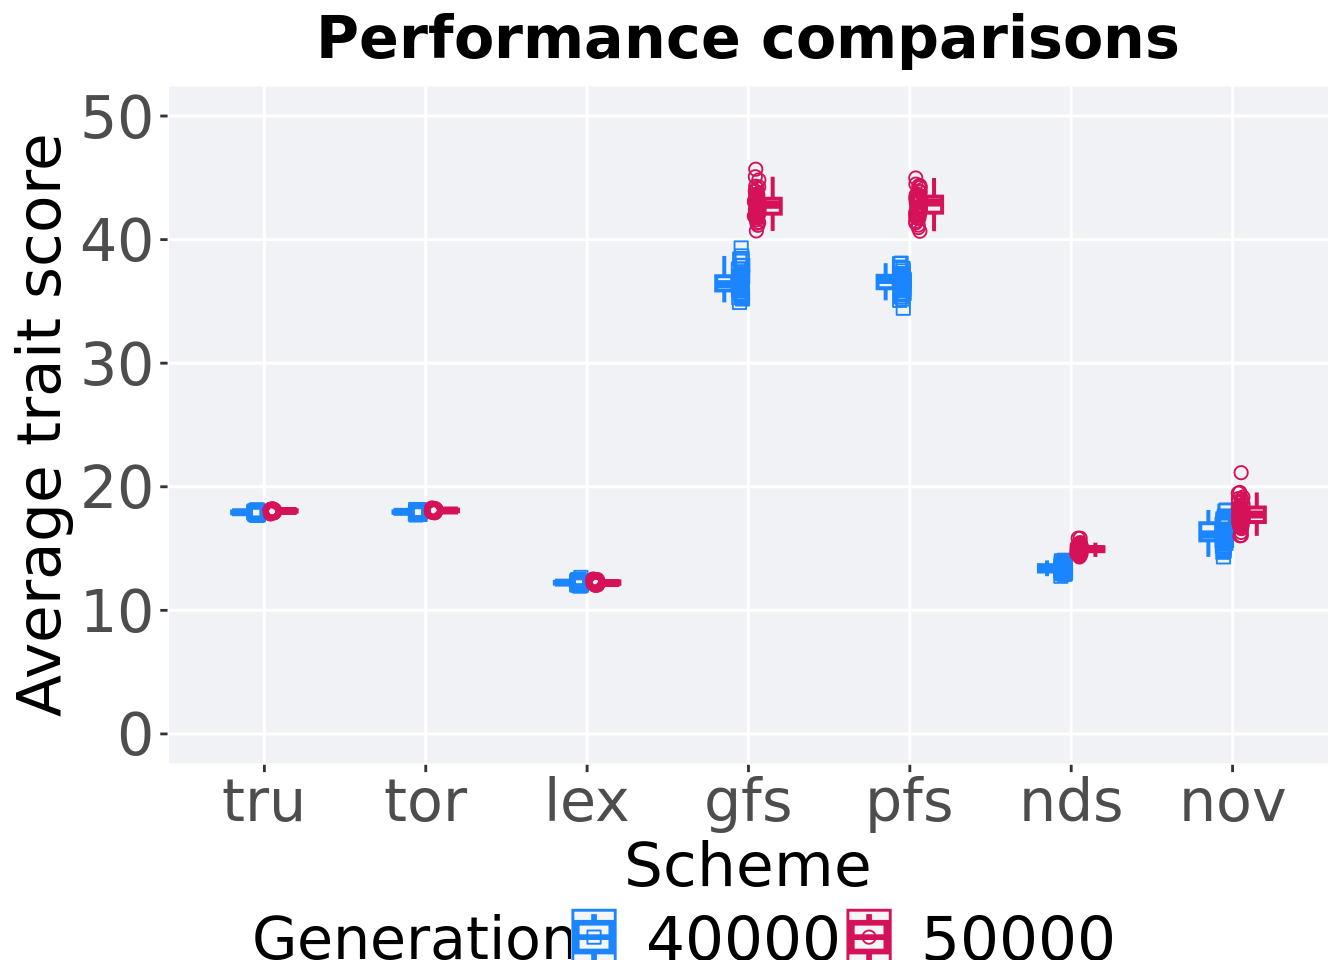
\includegraphics{demo_files/figure-latex/exp-mvc-per-sli-1.pdf}

\hypertarget{stats-3}{%
\subsubsection{Stats}\label{stats-3}}

Summary statistics for the performance of the best performance at 40,000 and 50,000 generations.

\begin{Shaded}
\begin{Highlighting}[]
\CommentTok{### performance comparisons and generation slices 40K & 50K}
\NormalTok{slices =}\StringTok{ }\KeywordTok{filter}\NormalTok{(cc_over_time_mvc, diagnostic }\OperatorTok{==}\StringTok{ 'exploitation_rate'} \OperatorTok{&}\StringTok{ }\NormalTok{(gen }\OperatorTok{==}\StringTok{ }\DecValTok{50000} \OperatorTok{|}\StringTok{ }\NormalTok{gen }\OperatorTok{==}\StringTok{ }\DecValTok{40000}\NormalTok{) }\OperatorTok{&}\StringTok{ }\NormalTok{acron }\OperatorTok{!=}\StringTok{ 'ran'}\NormalTok{)}
\NormalTok{slices}\OperatorTok{$}\NormalTok{Generation <-}\StringTok{ }\KeywordTok{factor}\NormalTok{(slices}\OperatorTok{$}\NormalTok{gen, }\DataTypeTok{levels =} \KeywordTok{c}\NormalTok{(}\DecValTok{50000}\NormalTok{,}\DecValTok{40000}\NormalTok{))}
\NormalTok{slices}\OperatorTok{$}\NormalTok{acron =}\StringTok{ }\KeywordTok{factor}\NormalTok{(slices}\OperatorTok{$}\NormalTok{acron, }\DataTypeTok{levels =} \KeywordTok{c}\NormalTok{(}\StringTok{'gfs'}\NormalTok{,}\StringTok{'pfs'}\NormalTok{,}\StringTok{'tru'}\NormalTok{,}\StringTok{'tor'}\NormalTok{,}\StringTok{'nov'}\NormalTok{, }\StringTok{'nds'}\NormalTok{,}\StringTok{'lex'}\NormalTok{, }\StringTok{'ran'}\NormalTok{))}
\NormalTok{slices }\OperatorTok
\StringTok{  }\KeywordTok{group_by}\NormalTok{(acron, Generation) }\OperatorTok
\StringTok{  }\NormalTok{dplyr}\OperatorTok{::}\KeywordTok{summarise}\NormalTok{(}
    \DataTypeTok{count =} \KeywordTok{n}\NormalTok{(),}
    \DataTypeTok{na_cnt =} \KeywordTok{sum}\NormalTok{(}\KeywordTok{is.na}\NormalTok{(pop_fit_max  }\OperatorTok{/}\StringTok{ }\NormalTok{DIMENSIONALITY)),}
    \DataTypeTok{min =} \KeywordTok{min}\NormalTok{(pop_fit_max  }\OperatorTok{/}\StringTok{ }\NormalTok{DIMENSIONALITY, }\DataTypeTok{na.rm =} \OtherTok{TRUE}\NormalTok{),}
    \DataTypeTok{median =} \KeywordTok{median}\NormalTok{(pop_fit_max  }\OperatorTok{/}\StringTok{ }\NormalTok{DIMENSIONALITY, }\DataTypeTok{na.rm =} \OtherTok{TRUE}\NormalTok{),}
    \DataTypeTok{mean =} \KeywordTok{mean}\NormalTok{(pop_fit_max  }\OperatorTok{/}\StringTok{ }\NormalTok{DIMENSIONALITY, }\DataTypeTok{na.rm =} \OtherTok{TRUE}\NormalTok{),}
    \DataTypeTok{max =} \KeywordTok{max}\NormalTok{(pop_fit_max  }\OperatorTok{/}\StringTok{ }\NormalTok{DIMENSIONALITY, }\DataTypeTok{na.rm =} \OtherTok{TRUE}\NormalTok{),}
    \DataTypeTok{IQR =} \KeywordTok{IQR}\NormalTok{(pop_fit_max  }\OperatorTok{/}\StringTok{ }\NormalTok{DIMENSIONALITY, }\DataTypeTok{na.rm =} \OtherTok{TRUE}\NormalTok{)}
\NormalTok{  )}
\end{Highlighting}
\end{Shaded}

\begin{verbatim}
## `summarise()` has grouped output by 'acron'. You can override using the
## `.groups` argument.
\end{verbatim}

\begin{verbatim}
## # A tibble: 14 x 9
## # Groups:   acron [7]
##    acron Generation count na_cnt   min median  mean   max   IQR
##    <fct> <fct>      <int>  <int> <dbl>  <dbl> <dbl> <dbl> <dbl>
##  1 gfs   50000         50      0  40.7   42.8  42.8  45.7 1.21 
##  2 gfs   40000         50      0  34.9   36.4  36.6  39.3 1.15 
##  3 pfs   50000         50      0  40.7   43.0  42.8  45.0 1.30 
##  4 pfs   40000         50      0  34.4   36.7  36.6  38.1 1.01 
##  5 tru   50000         50      0  17.8   18.0  18.0  18.2 0.118
##  6 tru   40000         50      0  17.7   17.9  17.9  18.1 0.147
##  7 tor   50000         50      0  17.9   18.1  18.1  18.3 0.130
##  8 tor   40000         50      0  17.7   18.0  18.0  18.2 0.115
##  9 nov   50000         50      0  16.0   17.8  17.8  21.1 1.17 
## 10 nov   40000         50      0  14.3   16.1  16.3  18.1 1.39 
## 11 nds   50000         50      0  14.3   15.0  15.0  15.8 0.327
## 12 nds   40000         50      0  12.8   13.4  13.4  14.0 0.516
## 13 lex   50000         50      0  12.0   12.2  12.2  12.5 0.199
## 14 lex   40000         50      0  12.0   12.2  12.2  12.7 0.132
\end{verbatim}

Truncation selection comparisons.

\begin{Shaded}
\begin{Highlighting}[]
\KeywordTok{wilcox.test}\NormalTok{(}\DataTypeTok{x =} \KeywordTok{filter}\NormalTok{(slices, acron }\OperatorTok{==}\StringTok{ 'tru'} \OperatorTok{&}\StringTok{ }\NormalTok{Generation }\OperatorTok{==}\StringTok{ }\DecValTok{50000}\NormalTok{)}\OperatorTok{$}\NormalTok{pop_fit_max,}
            \DataTypeTok{y =} \KeywordTok{filter}\NormalTok{(slices, acron }\OperatorTok{==}\StringTok{ 'tru'} \OperatorTok{&}\StringTok{ }\NormalTok{Generation }\OperatorTok{==}\StringTok{ }\DecValTok{40000}\NormalTok{)}\OperatorTok{$}\NormalTok{pop_fit_max,}
            \DataTypeTok{alternative =} \StringTok{'t'}\NormalTok{)}
\end{Highlighting}
\end{Shaded}

\begin{verbatim}
## 
##  Wilcoxon rank sum test with continuity correction
## 
## data:  filter(slices, acron == "tru" & Generation == 50000)$pop_fit_max and filter(slices, acron == "tru" & Generation == 40000)$pop_fit_max
## W = 2037.5, p-value = 5.705e-08
## alternative hypothesis: true location shift is not equal to 0
\end{verbatim}

Tournament selection comparisons.

\begin{Shaded}
\begin{Highlighting}[]
\KeywordTok{wilcox.test}\NormalTok{(}\DataTypeTok{x =} \KeywordTok{filter}\NormalTok{(slices, acron }\OperatorTok{==}\StringTok{ 'tor'} \OperatorTok{&}\StringTok{ }\NormalTok{Generation }\OperatorTok{==}\StringTok{ }\DecValTok{50000}\NormalTok{)}\OperatorTok{$}\NormalTok{pop_fit_max,}
            \DataTypeTok{y =} \KeywordTok{filter}\NormalTok{(slices, acron }\OperatorTok{==}\StringTok{ 'tor'} \OperatorTok{&}\StringTok{ }\NormalTok{Generation }\OperatorTok{==}\StringTok{ }\DecValTok{40000}\NormalTok{)}\OperatorTok{$}\NormalTok{pop_fit_max,}
            \DataTypeTok{alternative =} \StringTok{'t'}\NormalTok{)}
\end{Highlighting}
\end{Shaded}

\begin{verbatim}
## 
##  Wilcoxon rank sum test with continuity correction
## 
## data:  filter(slices, acron == "tor" & Generation == 50000)$pop_fit_max and filter(slices, acron == "tor" & Generation == 40000)$pop_fit_max
## W = 2075, p-value = 1.301e-08
## alternative hypothesis: true location shift is not equal to 0
\end{verbatim}

Lexicase selection comparisons.

\begin{Shaded}
\begin{Highlighting}[]
\KeywordTok{wilcox.test}\NormalTok{(}\DataTypeTok{x =} \KeywordTok{filter}\NormalTok{(slices, acron }\OperatorTok{==}\StringTok{ 'lex'} \OperatorTok{&}\StringTok{ }\NormalTok{Generation }\OperatorTok{==}\StringTok{ }\DecValTok{50000}\NormalTok{)}\OperatorTok{$}\NormalTok{pop_fit_max,}
            \DataTypeTok{y =} \KeywordTok{filter}\NormalTok{(slices, acron }\OperatorTok{==}\StringTok{ 'lex'} \OperatorTok{&}\StringTok{ }\NormalTok{Generation }\OperatorTok{==}\StringTok{ }\DecValTok{40000}\NormalTok{)}\OperatorTok{$}\NormalTok{pop_fit_max,}
            \DataTypeTok{alternative =} \StringTok{'t'}\NormalTok{)}
\end{Highlighting}
\end{Shaded}

\begin{verbatim}
## 
##  Wilcoxon rank sum test with continuity correction
## 
## data:  filter(slices, acron == "lex" & Generation == 50000)$pop_fit_max and filter(slices, acron == "lex" & Generation == 40000)$pop_fit_max
## W = 1260.5, p-value = 0.945
## alternative hypothesis: true location shift is not equal to 0
\end{verbatim}

Genotypic fitness sharing comparisons.

\begin{Shaded}
\begin{Highlighting}[]
\KeywordTok{wilcox.test}\NormalTok{(}\DataTypeTok{x =} \KeywordTok{filter}\NormalTok{(slices, acron }\OperatorTok{==}\StringTok{ 'gfs'} \OperatorTok{&}\StringTok{ }\NormalTok{Generation }\OperatorTok{==}\StringTok{ }\DecValTok{50000}\NormalTok{)}\OperatorTok{$}\NormalTok{pop_fit_max,}
            \DataTypeTok{y =} \KeywordTok{filter}\NormalTok{(slices, acron }\OperatorTok{==}\StringTok{ 'gfs'} \OperatorTok{&}\StringTok{ }\NormalTok{Generation }\OperatorTok{==}\StringTok{ }\DecValTok{40000}\NormalTok{)}\OperatorTok{$}\NormalTok{pop_fit_max,}
            \DataTypeTok{alternative =} \StringTok{'t'}\NormalTok{)}
\end{Highlighting}
\end{Shaded}

\begin{verbatim}
## 
##  Wilcoxon rank sum test with continuity correction
## 
## data:  filter(slices, acron == "gfs" & Generation == 50000)$pop_fit_max and filter(slices, acron == "gfs" & Generation == 40000)$pop_fit_max
## W = 2500, p-value < 2.2e-16
## alternative hypothesis: true location shift is not equal to 0
\end{verbatim}

Phenotypic fitness sharing comparisons.

\begin{Shaded}
\begin{Highlighting}[]
\KeywordTok{wilcox.test}\NormalTok{(}\DataTypeTok{x =} \KeywordTok{filter}\NormalTok{(slices, acron }\OperatorTok{==}\StringTok{ 'pfs'} \OperatorTok{&}\StringTok{ }\NormalTok{Generation }\OperatorTok{==}\StringTok{ }\DecValTok{50000}\NormalTok{)}\OperatorTok{$}\NormalTok{pop_fit_max,}
            \DataTypeTok{y =} \KeywordTok{filter}\NormalTok{(slices, acron }\OperatorTok{==}\StringTok{ 'pfs'} \OperatorTok{&}\StringTok{ }\NormalTok{Generation }\OperatorTok{==}\StringTok{ }\DecValTok{40000}\NormalTok{)}\OperatorTok{$}\NormalTok{pop_fit_max,}
            \DataTypeTok{alternative =} \StringTok{'t'}\NormalTok{)}
\end{Highlighting}
\end{Shaded}

\begin{verbatim}
## 
##  Wilcoxon rank sum test with continuity correction
## 
## data:  filter(slices, acron == "pfs" & Generation == 50000)$pop_fit_max and filter(slices, acron == "pfs" & Generation == 40000)$pop_fit_max
## W = 2500, p-value < 2.2e-16
## alternative hypothesis: true location shift is not equal to 0
\end{verbatim}

Nondominated sorting comparisons.

\begin{Shaded}
\begin{Highlighting}[]
\KeywordTok{wilcox.test}\NormalTok{(}\DataTypeTok{x =} \KeywordTok{filter}\NormalTok{(slices, acron }\OperatorTok{==}\StringTok{ 'nds'} \OperatorTok{&}\StringTok{ }\NormalTok{Generation }\OperatorTok{==}\StringTok{ }\DecValTok{50000}\NormalTok{)}\OperatorTok{$}\NormalTok{pop_fit_max,}
            \DataTypeTok{y =} \KeywordTok{filter}\NormalTok{(slices, acron }\OperatorTok{==}\StringTok{ 'nds'} \OperatorTok{&}\StringTok{ }\NormalTok{Generation }\OperatorTok{==}\StringTok{ }\DecValTok{40000}\NormalTok{)}\OperatorTok{$}\NormalTok{pop_fit_max,}
            \DataTypeTok{alternative =} \StringTok{'t'}\NormalTok{)}
\end{Highlighting}
\end{Shaded}

\begin{verbatim}
## 
##  Wilcoxon rank sum test with continuity correction
## 
## data:  filter(slices, acron == "nds" & Generation == 50000)$pop_fit_max and filter(slices, acron == "nds" & Generation == 40000)$pop_fit_max
## W = 2500, p-value < 2.2e-16
## alternative hypothesis: true location shift is not equal to 0
\end{verbatim}

Novelty search comparisons.

\begin{Shaded}
\begin{Highlighting}[]
\KeywordTok{wilcox.test}\NormalTok{(}\DataTypeTok{x =} \KeywordTok{filter}\NormalTok{(slices, acron }\OperatorTok{==}\StringTok{ 'nov'} \OperatorTok{&}\StringTok{ }\NormalTok{Generation }\OperatorTok{==}\StringTok{ }\DecValTok{50000}\NormalTok{)}\OperatorTok{$}\NormalTok{pop_fit_max,}
            \DataTypeTok{y =} \KeywordTok{filter}\NormalTok{(slices, acron }\OperatorTok{==}\StringTok{ 'nov'} \OperatorTok{&}\StringTok{ }\NormalTok{Generation }\OperatorTok{==}\StringTok{ }\DecValTok{40000}\NormalTok{)}\OperatorTok{$}\NormalTok{pop_fit_max,}
            \DataTypeTok{alternative =} \StringTok{'t'}\NormalTok{)}
\end{Highlighting}
\end{Shaded}

\begin{verbatim}
## 
##  Wilcoxon rank sum test with continuity correction
## 
## data:  filter(slices, acron == "nov" & Generation == 50000)$pop_fit_max and filter(slices, acron == "nov" & Generation == 40000)$pop_fit_max
## W = 2196, p-value = 7.119e-11
## alternative hypothesis: true location shift is not equal to 0
\end{verbatim}

\hypertarget{exploitation-rate-results-1}{%
\chapter{Exploitation rate results}\label{exploitation-rate-results-1}}

Here we present the results for \textbf{best performances} found by each selection scheme replicate on the ordered exploitation diagnostic.
Best performance found refers to the largest average trait score found in a given population.
Note that performance values fall between 0.0 and 100.0.

\hypertarget{analysis-dependencies-1}{%
\section{Analysis dependencies}\label{analysis-dependencies-1}}

\begin{Shaded}
\begin{Highlighting}[]
\KeywordTok{library}\NormalTok{(ggplot2)}
\KeywordTok{library}\NormalTok{(cowplot)}
\KeywordTok{library}\NormalTok{(dplyr)}
\KeywordTok{library}\NormalTok{(PupillometryR)}
\KeywordTok{library}\NormalTok{(sdamr)}
\end{Highlighting}
\end{Shaded}

\hypertarget{performance-over-time-2}{%
\section{Performance over time}\label{performance-over-time-2}}

Best performance in a population over time.

\begin{Shaded}
\begin{Highlighting}[]
\CommentTok{# data for lines and shading on plots}
\NormalTok{lines =}\StringTok{ }\KeywordTok{filter}\NormalTok{(cc_over_time, diagnostic }\OperatorTok{==}\StringTok{ 'ordered_exploitation'}\NormalTok{) }\OperatorTok
\StringTok{  }\KeywordTok{group_by}\NormalTok{(}\StringTok{`}\DataTypeTok{Selection}\CharTok{\textbackslash{}n}\DataTypeTok{Scheme}\StringTok{`}\NormalTok{, gen) }\OperatorTok
\StringTok{  }\NormalTok{dplyr}\OperatorTok{::}\KeywordTok{summarise}\NormalTok{(}
    \DataTypeTok{min =} \KeywordTok{min}\NormalTok{(pop_fit_max) }\OperatorTok{/}\StringTok{ }\NormalTok{DIMENSIONALITY,}
    \DataTypeTok{mean =} \KeywordTok{mean}\NormalTok{(pop_fit_max) }\OperatorTok{/}\StringTok{ }\NormalTok{DIMENSIONALITY,}
    \DataTypeTok{max =} \KeywordTok{max}\NormalTok{(pop_fit_max) }\OperatorTok{/}\StringTok{ }\NormalTok{DIMENSIONALITY}
\NormalTok{  )}
\end{Highlighting}
\end{Shaded}

\begin{verbatim}
## `summarise()` has grouped output by 'Selection Scheme'. You can override using
## the `.groups` argument.
\end{verbatim}

\begin{Shaded}
\begin{Highlighting}[]
\KeywordTok{ggplot}\NormalTok{(lines, }\KeywordTok{aes}\NormalTok{(}\DataTypeTok{x=}\NormalTok{gen, }\DataTypeTok{y=}\NormalTok{mean, }\DataTypeTok{group =} \StringTok{`}\DataTypeTok{Selection}\CharTok{\textbackslash{}n}\DataTypeTok{Scheme}\StringTok{`}\NormalTok{, }\DataTypeTok{fill =}\StringTok{`}\DataTypeTok{Selection}\CharTok{\textbackslash{}n}\DataTypeTok{Scheme}\StringTok{`}\NormalTok{, }\DataTypeTok{color =} \StringTok{`}\DataTypeTok{Selection}\CharTok{\textbackslash{}n}\DataTypeTok{Scheme}\StringTok{`}\NormalTok{, }\DataTypeTok{shape =} \StringTok{`}\DataTypeTok{Selection}\CharTok{\textbackslash{}n}\DataTypeTok{Scheme}\StringTok{`}\NormalTok{)) }\OperatorTok{+}
\StringTok{  }\KeywordTok{geom_ribbon}\NormalTok{(}\KeywordTok{aes}\NormalTok{(}\DataTypeTok{ymin =}\NormalTok{ min, }\DataTypeTok{ymax =}\NormalTok{ max), }\DataTypeTok{alpha =} \FloatTok{0.1}\NormalTok{) }\OperatorTok{+}
\StringTok{  }\KeywordTok{geom_line}\NormalTok{(}\DataTypeTok{size =} \FloatTok{0.5}\NormalTok{) }\OperatorTok{+}
\StringTok{  }\KeywordTok{geom_point}\NormalTok{(}\DataTypeTok{data =} \KeywordTok{filter}\NormalTok{(lines, gen }\OperatorTok\StringTok{ }\DecValTok{2000} \OperatorTok{==}\StringTok{ }\DecValTok{0} \OperatorTok{&}\StringTok{ }\NormalTok{gen }\OperatorTok{!=}\StringTok{ }\DecValTok{0}\NormalTok{), }\DataTypeTok{size =} \FloatTok{1.5}\NormalTok{, }\DataTypeTok{stroke =} \FloatTok{2.0}\NormalTok{, }\DataTypeTok{alpha =} \FloatTok{1.0}\NormalTok{) }\OperatorTok{+}
\StringTok{  }\KeywordTok{scale_y_continuous}\NormalTok{(}
    \DataTypeTok{name=}\StringTok{"Average trait score"}\NormalTok{,}
    \DataTypeTok{limits=}\KeywordTok{c}\NormalTok{(}\DecValTok{0}\NormalTok{, }\DecValTok{100}\NormalTok{),}
    \DataTypeTok{breaks=}\KeywordTok{seq}\NormalTok{(}\DecValTok{0}\NormalTok{,}\DecValTok{100}\NormalTok{, }\DecValTok{20}\NormalTok{),}
    \DataTypeTok{labels=}\KeywordTok{c}\NormalTok{(}\StringTok{"0"}\NormalTok{, }\StringTok{"20"}\NormalTok{, }\StringTok{"40"}\NormalTok{, }\StringTok{"60"}\NormalTok{, }\StringTok{"80"}\NormalTok{, }\StringTok{"100"}\NormalTok{)}
\NormalTok{  ) }\OperatorTok{+}
\StringTok{  }\KeywordTok{scale_x_continuous}\NormalTok{(}
    \DataTypeTok{name=}\StringTok{"Generations"}\NormalTok{,}
    \DataTypeTok{limits=}\KeywordTok{c}\NormalTok{(}\DecValTok{0}\NormalTok{, }\DecValTok{50000}\NormalTok{),}
    \DataTypeTok{breaks=}\KeywordTok{c}\NormalTok{(}\DecValTok{0}\NormalTok{, }\DecValTok{10000}\NormalTok{, }\DecValTok{20000}\NormalTok{, }\DecValTok{30000}\NormalTok{, }\DecValTok{40000}\NormalTok{, }\DecValTok{50000}\NormalTok{),}
    \DataTypeTok{labels=}\KeywordTok{c}\NormalTok{(}\StringTok{"0e+4"}\NormalTok{, }\StringTok{"1e+4"}\NormalTok{, }\StringTok{"2e+4"}\NormalTok{, }\StringTok{"3e+4"}\NormalTok{, }\StringTok{"4e+4"}\NormalTok{, }\StringTok{"5e+4"}\NormalTok{)}

\NormalTok{  ) }\OperatorTok{+}
\StringTok{  }\KeywordTok{scale_shape_manual}\NormalTok{(}\DataTypeTok{values=}\NormalTok{SHAPE)}\OperatorTok{+}
\StringTok{  }\KeywordTok{scale_colour_manual}\NormalTok{(}\DataTypeTok{values =}\NormalTok{ cb_palette) }\OperatorTok{+}
\StringTok{  }\KeywordTok{scale_fill_manual}\NormalTok{(}\DataTypeTok{values =}\NormalTok{ cb_palette) }\OperatorTok{+}
\StringTok{  }\KeywordTok{ggtitle}\NormalTok{(}\StringTok{'Performance over time'}\NormalTok{)}\OperatorTok{+}
\StringTok{  }\NormalTok{p_theme }\OperatorTok{+}\StringTok{ }\KeywordTok{theme}\NormalTok{(}\DataTypeTok{legend.title=}\KeywordTok{element_blank}\NormalTok{(),}\DataTypeTok{legend.text=}\KeywordTok{element_text}\NormalTok{(}\DataTypeTok{size=}\DecValTok{12}\NormalTok{)) }\OperatorTok{+}
\StringTok{  }\KeywordTok{guides}\NormalTok{(}
    \DataTypeTok{shape=}\KeywordTok{guide_legend}\NormalTok{(}\DataTypeTok{ncol=}\DecValTok{2}\NormalTok{, }\DataTypeTok{title.position =} \StringTok{"bottom"}\NormalTok{),}
    \DataTypeTok{color=}\KeywordTok{guide_legend}\NormalTok{(}\DataTypeTok{ncol=}\DecValTok{2}\NormalTok{, }\DataTypeTok{title.position =} \StringTok{"bottom"}\NormalTok{),}
    \DataTypeTok{fill=}\KeywordTok{guide_legend}\NormalTok{(}\DataTypeTok{ncol=}\DecValTok{2}\NormalTok{, }\DataTypeTok{title.position =} \StringTok{"bottom"}\NormalTok{)}
\NormalTok{  )}
\end{Highlighting}
\end{Shaded}

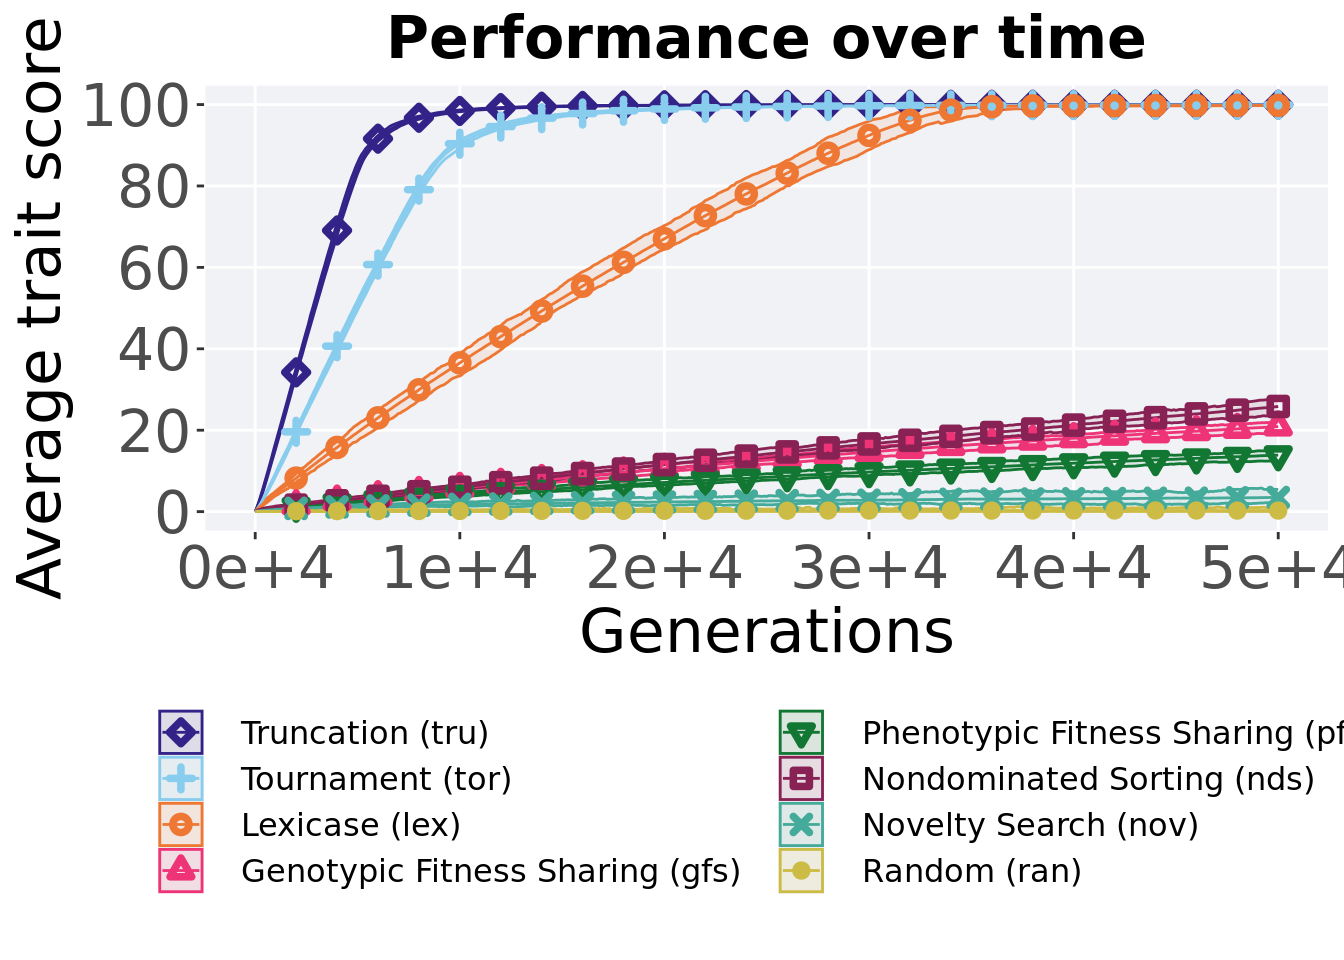
\includegraphics{demo_files/figure-latex/ord-per-ot-1.pdf}

\hypertarget{best-performance-throughout-2}{%
\section{Best performance throughout}\label{best-performance-throughout-2}}

Best performance found throughout 50,000 generations.

\begin{Shaded}
\begin{Highlighting}[]
\CommentTok{### best performance throughout}
\KeywordTok{filter}\NormalTok{(cc_best, col }\OperatorTok{==}\StringTok{ 'pop_fit_max'} \OperatorTok{&}\StringTok{ }\NormalTok{diagnostic }\OperatorTok{==}\StringTok{ 'ordered_exploitation'}\NormalTok{) }\OperatorTok
\StringTok{  }\KeywordTok{ggplot}\NormalTok{(., }\KeywordTok{aes}\NormalTok{(}\DataTypeTok{x =}\NormalTok{ acron, }\DataTypeTok{y =}\NormalTok{ val }\OperatorTok{/}\StringTok{ }\NormalTok{DIMENSIONALITY, }\DataTypeTok{color =}\NormalTok{ acron, }\DataTypeTok{fill =}\NormalTok{ acron, }\DataTypeTok{shape =}\NormalTok{ acron)) }\OperatorTok{+}
\StringTok{  }\KeywordTok{geom_flat_violin}\NormalTok{(}\DataTypeTok{position =} \KeywordTok{position_nudge}\NormalTok{(}\DataTypeTok{x =} \FloatTok{.2}\NormalTok{, }\DataTypeTok{y =} \DecValTok{0}\NormalTok{), }\DataTypeTok{scale =} \StringTok{'width'}\NormalTok{, }\DataTypeTok{alpha =} \FloatTok{0.2}\NormalTok{) }\OperatorTok{+}
\StringTok{  }\KeywordTok{geom_point}\NormalTok{(}\DataTypeTok{position =} \KeywordTok{position_jitter}\NormalTok{(}\DataTypeTok{width =} \FloatTok{.1}\NormalTok{), }\DataTypeTok{size =} \FloatTok{1.5}\NormalTok{, }\DataTypeTok{alpha =} \FloatTok{1.0}\NormalTok{) }\OperatorTok{+}
\StringTok{  }\KeywordTok{geom_boxplot}\NormalTok{(}\DataTypeTok{color =} \StringTok{'black'}\NormalTok{, }\DataTypeTok{width =} \FloatTok{.2}\NormalTok{, }\DataTypeTok{outlier.shape =} \OtherTok{NA}\NormalTok{, }\DataTypeTok{alpha =} \FloatTok{0.0}\NormalTok{) }\OperatorTok{+}
\StringTok{  }\KeywordTok{scale_y_continuous}\NormalTok{(}
    \DataTypeTok{name=}\StringTok{"Average trait score"}\NormalTok{,}
    \DataTypeTok{limits=}\KeywordTok{c}\NormalTok{(}\OperatorTok{-}\DecValTok{1}\NormalTok{, }\DecValTok{101}\NormalTok{),}
    \DataTypeTok{breaks=}\KeywordTok{seq}\NormalTok{(}\DecValTok{0}\NormalTok{,}\DecValTok{100}\NormalTok{, }\DecValTok{20}\NormalTok{),}
    \DataTypeTok{labels=}\KeywordTok{c}\NormalTok{(}\StringTok{"0"}\NormalTok{, }\StringTok{"20"}\NormalTok{, }\StringTok{"40"}\NormalTok{, }\StringTok{"60"}\NormalTok{, }\StringTok{"80"}\NormalTok{, }\StringTok{"100"}\NormalTok{)}
\NormalTok{  ) }\OperatorTok{+}
\StringTok{  }\KeywordTok{scale_x_discrete}\NormalTok{(}
    \DataTypeTok{name=}\StringTok{"Scheme"}
\NormalTok{  )}\OperatorTok{+}
\StringTok{  }\KeywordTok{scale_shape_manual}\NormalTok{(}\DataTypeTok{values=}\NormalTok{SHAPE)}\OperatorTok{+}
\StringTok{  }\KeywordTok{scale_colour_manual}\NormalTok{(}\DataTypeTok{values =}\NormalTok{ cb_palette, ) }\OperatorTok{+}
\StringTok{  }\KeywordTok{scale_fill_manual}\NormalTok{(}\DataTypeTok{values =}\NormalTok{ cb_palette) }\OperatorTok{+}
\StringTok{  }\KeywordTok{ggtitle}\NormalTok{(}\StringTok{'Best performance throughout'}\NormalTok{)}\OperatorTok{+}
\StringTok{  }\NormalTok{p_theme }\OperatorTok{+}\StringTok{ }\KeywordTok{theme}\NormalTok{(}\DataTypeTok{legend.title=}\KeywordTok{element_blank}\NormalTok{()) }\OperatorTok{+}
\StringTok{  }\KeywordTok{guides}\NormalTok{(}
    \DataTypeTok{shape=}\KeywordTok{guide_legend}\NormalTok{(}\DataTypeTok{nrow=}\DecValTok{2}\NormalTok{, }\DataTypeTok{title.position =} \StringTok{"bottom"}\NormalTok{),}
    \DataTypeTok{color=}\KeywordTok{guide_legend}\NormalTok{(}\DataTypeTok{nrow=}\DecValTok{2}\NormalTok{, }\DataTypeTok{title.position =} \StringTok{"bottom"}\NormalTok{),}
    \DataTypeTok{fill=}\KeywordTok{guide_legend}\NormalTok{(}\DataTypeTok{nrow=}\DecValTok{2}\NormalTok{, }\DataTypeTok{title.position =} \StringTok{"bottom"}\NormalTok{)}
\NormalTok{  )}
\end{Highlighting}
\end{Shaded}

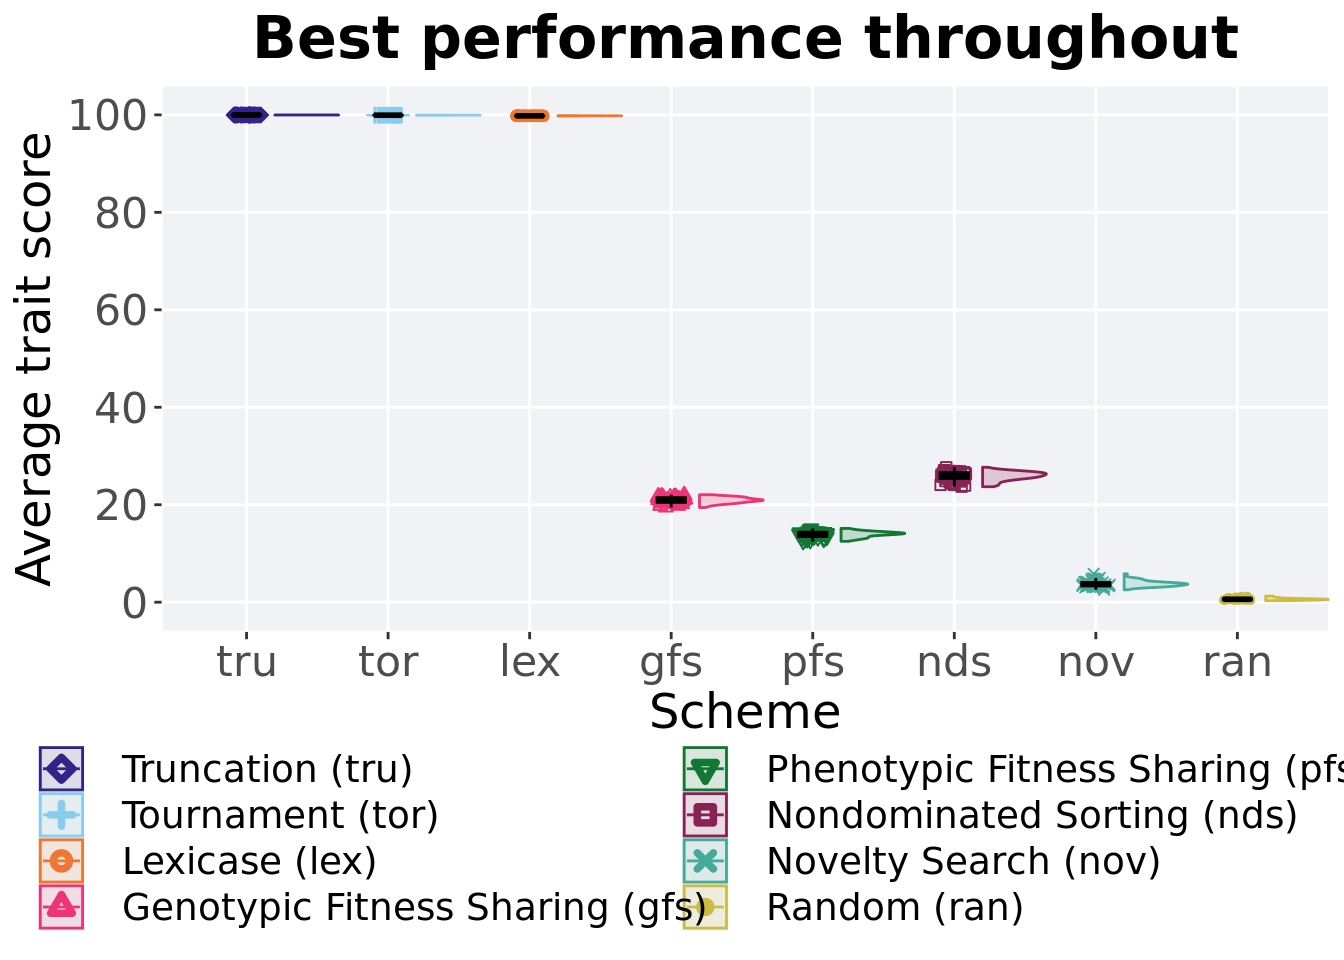
\includegraphics{demo_files/figure-latex/ord-per-bst-1.pdf}

\hypertarget{stats-4}{%
\subsection{Stats}\label{stats-4}}

Summary statistics for the performance of the best performance throughout 50,000 generations.

\begin{Shaded}
\begin{Highlighting}[]
\CommentTok{#get data & summarize}
\NormalTok{performance =}\StringTok{ }\KeywordTok{filter}\NormalTok{(cc_best, col }\OperatorTok{==}\StringTok{ 'pop_fit_max'} \OperatorTok{&}\StringTok{ }\NormalTok{diagnostic }\OperatorTok{==}\StringTok{ 'ordered_exploitation'}\NormalTok{)}
\NormalTok{performance}\OperatorTok{$}\NormalTok{acron =}\StringTok{ }\KeywordTok{factor}\NormalTok{(performance}\OperatorTok{$}\NormalTok{acron, }\DataTypeTok{levels =} \KeywordTok{c}\NormalTok{(}\StringTok{'tru'}\NormalTok{, }\StringTok{'tor'}\NormalTok{, }\StringTok{'lex'}\NormalTok{,}\StringTok{'nds'}\NormalTok{, }\StringTok{'gfs'}\NormalTok{, }\StringTok{'pfs'}\NormalTok{, }\StringTok{'nov'}\NormalTok{,  }\StringTok{'ran'}\NormalTok{))}
\NormalTok{performance }\OperatorTok
\StringTok{  }\KeywordTok{group_by}\NormalTok{(acron) }\OperatorTok
\StringTok{  }\NormalTok{dplyr}\OperatorTok{::}\KeywordTok{summarise}\NormalTok{(}
    \DataTypeTok{count =} \KeywordTok{n}\NormalTok{(),}
    \DataTypeTok{na_cnt =} \KeywordTok{sum}\NormalTok{(}\KeywordTok{is.na}\NormalTok{(val)),}
    \DataTypeTok{min =} \KeywordTok{min}\NormalTok{(val }\OperatorTok{/}\StringTok{ }\NormalTok{DIMENSIONALITY, }\DataTypeTok{na.rm =} \OtherTok{TRUE}\NormalTok{),}
    \DataTypeTok{median =} \KeywordTok{median}\NormalTok{(val }\OperatorTok{/}\StringTok{ }\NormalTok{DIMENSIONALITY, }\DataTypeTok{na.rm =} \OtherTok{TRUE}\NormalTok{),}
    \DataTypeTok{mean =} \KeywordTok{mean}\NormalTok{(val }\OperatorTok{/}\StringTok{ }\NormalTok{DIMENSIONALITY, }\DataTypeTok{na.rm =} \OtherTok{TRUE}\NormalTok{),}
    \DataTypeTok{max =} \KeywordTok{max}\NormalTok{(val }\OperatorTok{/}\StringTok{ }\NormalTok{DIMENSIONALITY, }\DataTypeTok{na.rm =} \OtherTok{TRUE}\NormalTok{),}
    \DataTypeTok{IQR =} \KeywordTok{IQR}\NormalTok{(val }\OperatorTok{/}\StringTok{ }\NormalTok{DIMENSIONALITY, }\DataTypeTok{na.rm =} \OtherTok{TRUE}\NormalTok{)}
\NormalTok{  )}
\end{Highlighting}
\end{Shaded}

\begin{verbatim}
## # A tibble: 8 x 8
##   acron count na_cnt     min  median    mean    max     IQR
##   <fct> <int>  <int>   <dbl>   <dbl>   <dbl>  <dbl>   <dbl>
## 1 tru      50      0 100.    100.    100.    100.   0.00208
## 2 tor      50      0  99.9    99.9    99.9    99.9  0.00445
## 3 lex      50      0  99.8    99.8    99.8    99.8  0.0207 
## 4 nds      50      0  23.7    26.0    25.9    27.7  1.17   
## 5 gfs      50      0  19.4    21.0    20.9    22.1  0.970  
## 6 pfs      50      0  12.5    14.1    13.9    15.1  0.871  
## 7 nov      50      0   2.55    3.70    3.80    5.82 0.718  
## 8 ran      50      0   0.319   0.598   0.634   1.26 0.240
\end{verbatim}

Kruskal--Wallis test provides evidence of statistical differences.

\begin{Shaded}
\begin{Highlighting}[]
\KeywordTok{kruskal.test}\NormalTok{(val }\OperatorTok{~}\StringTok{ }\NormalTok{acron, }\DataTypeTok{data =}\NormalTok{ performance)}
\end{Highlighting}
\end{Shaded}

\begin{verbatim}
## 
##  Kruskal-Wallis rank sum test
## 
## data:  val by acron
## Kruskal-Wallis chi-squared = 392.77, df = 7, p-value < 2.2e-16
\end{verbatim}

Results for post-hoc Wilcoxon rank-sum test with a Bonferroni correction.

\begin{Shaded}
\begin{Highlighting}[]
\KeywordTok{pairwise.wilcox.test}\NormalTok{(}\DataTypeTok{x =}\NormalTok{ performance}\OperatorTok{$}\NormalTok{val, }\DataTypeTok{g =}\NormalTok{ performance}\OperatorTok{$}\NormalTok{acron, }\DataTypeTok{p.adjust.method =} \StringTok{"bonferroni"}\NormalTok{,}
                     \DataTypeTok{paired =} \OtherTok{FALSE}\NormalTok{, }\DataTypeTok{conf.int =} \OtherTok{FALSE}\NormalTok{, }\DataTypeTok{alternative =} \StringTok{'l'}\NormalTok{)}
\end{Highlighting}
\end{Shaded}

\begin{verbatim}
## 
##  Pairwise comparisons using Wilcoxon rank sum test with continuity correction 
## 
## data:  performance$val and performance$acron 
## 
##     tru    tor    lex    nds    gfs    pfs    nov   
## tor <2e-16 -      -      -      -      -      -     
## lex <2e-16 <2e-16 -      -      -      -      -     
## nds <2e-16 <2e-16 <2e-16 -      -      -      -     
## gfs <2e-16 <2e-16 <2e-16 <2e-16 -      -      -     
## pfs <2e-16 <2e-16 <2e-16 <2e-16 <2e-16 -      -     
## nov <2e-16 <2e-16 <2e-16 <2e-16 <2e-16 <2e-16 -     
## ran <2e-16 <2e-16 <2e-16 <2e-16 <2e-16 <2e-16 <2e-16
## 
## P value adjustment method: bonferroni
\end{verbatim}

\hypertarget{generation-satisfactory-solution-found-1}{%
\section{Generation satisfactory solution found}\label{generation-satisfactory-solution-found-1}}

First generation a satisfactory solution is found throughout the 50,000 generations.

\begin{Shaded}
\begin{Highlighting}[]
\CommentTok{### satisfactory solution found}
\KeywordTok{filter}\NormalTok{(cc_ssf, diagnostic }\OperatorTok{==}\StringTok{ 'ordered_exploitation'}\NormalTok{) }\OperatorTok
\StringTok{  }\KeywordTok{ggplot}\NormalTok{(., }\KeywordTok{aes}\NormalTok{(}\DataTypeTok{x =}\NormalTok{ acron, }\DataTypeTok{y =}\NormalTok{ Generations , }\DataTypeTok{color =}\NormalTok{ acron, }\DataTypeTok{fill =}\NormalTok{ acron, }\DataTypeTok{shape =}\NormalTok{ acron)) }\OperatorTok{+}
\StringTok{  }\KeywordTok{geom_flat_violin}\NormalTok{(}\DataTypeTok{position =} \KeywordTok{position_nudge}\NormalTok{(}\DataTypeTok{x =} \FloatTok{.2}\NormalTok{, }\DataTypeTok{y =} \DecValTok{0}\NormalTok{), }\DataTypeTok{scale =} \StringTok{'width'}\NormalTok{, }\DataTypeTok{alpha =} \FloatTok{0.2}\NormalTok{) }\OperatorTok{+}
\StringTok{  }\KeywordTok{geom_point}\NormalTok{(}\DataTypeTok{position =} \KeywordTok{position_jitter}\NormalTok{(}\DataTypeTok{width =} \FloatTok{.1}\NormalTok{), }\DataTypeTok{size =} \FloatTok{1.5}\NormalTok{, }\DataTypeTok{alpha =} \FloatTok{1.0}\NormalTok{) }\OperatorTok{+}
\StringTok{  }\KeywordTok{geom_boxplot}\NormalTok{(}\DataTypeTok{color =} \StringTok{'black'}\NormalTok{, }\DataTypeTok{width =} \FloatTok{.2}\NormalTok{, }\DataTypeTok{outlier.shape =} \OtherTok{NA}\NormalTok{, }\DataTypeTok{alpha =} \FloatTok{0.0}\NormalTok{) }\OperatorTok{+}
\StringTok{  }\KeywordTok{scale_y_continuous}\NormalTok{(}
    \DataTypeTok{name=}\StringTok{"Generation"}\NormalTok{,}
    \DataTypeTok{limits=}\KeywordTok{c}\NormalTok{(}\DecValTok{0}\NormalTok{, }\DecValTok{60001}\NormalTok{),}
    \DataTypeTok{breaks=}\KeywordTok{c}\NormalTok{(}\DecValTok{0}\NormalTok{, }\DecValTok{10000}\NormalTok{, }\DecValTok{20000}\NormalTok{, }\DecValTok{30000}\NormalTok{, }\DecValTok{40000}\NormalTok{, }\DecValTok{50000}\NormalTok{, }\DecValTok{60000}\NormalTok{),}
    \DataTypeTok{labels=}\KeywordTok{c}\NormalTok{(}\StringTok{"0e+4"}\NormalTok{, }\StringTok{"1e+4"}\NormalTok{, }\StringTok{"2e+4"}\NormalTok{, }\StringTok{"3e+4"}\NormalTok{, }\StringTok{"4e+4"}\NormalTok{, }\StringTok{"5e+4"}\NormalTok{, }\StringTok{"Fail"}\NormalTok{)}
\NormalTok{  ) }\OperatorTok{+}
\StringTok{  }\KeywordTok{scale_x_discrete}\NormalTok{(}
    \DataTypeTok{name=}\StringTok{"Scheme"}
\NormalTok{  )}\OperatorTok{+}
\StringTok{  }\KeywordTok{scale_shape_manual}\NormalTok{(}\DataTypeTok{values=}\NormalTok{SHAPE)}\OperatorTok{+}
\StringTok{  }\KeywordTok{scale_colour_manual}\NormalTok{(}\DataTypeTok{values =}\NormalTok{ cb_palette, ) }\OperatorTok{+}
\StringTok{  }\KeywordTok{scale_fill_manual}\NormalTok{(}\DataTypeTok{values =}\NormalTok{ cb_palette) }\OperatorTok{+}
\StringTok{  }\KeywordTok{ggtitle}\NormalTok{(}\StringTok{'Generation satisfactory solution found'}\NormalTok{)}\OperatorTok{+}
\StringTok{  }\NormalTok{p_theme }\OperatorTok{+}\StringTok{ }\KeywordTok{theme}\NormalTok{(}\DataTypeTok{legend.title=}\KeywordTok{element_blank}\NormalTok{()) }\OperatorTok{+}
\StringTok{  }\KeywordTok{guides}\NormalTok{(}
    \DataTypeTok{shape=}\KeywordTok{guide_legend}\NormalTok{(}\DataTypeTok{nrow=}\DecValTok{2}\NormalTok{, }\DataTypeTok{title.position =} \StringTok{"bottom"}\NormalTok{),}
    \DataTypeTok{color=}\KeywordTok{guide_legend}\NormalTok{(}\DataTypeTok{nrow=}\DecValTok{2}\NormalTok{, }\DataTypeTok{title.position =} \StringTok{"bottom"}\NormalTok{),}
    \DataTypeTok{fill=}\KeywordTok{guide_legend}\NormalTok{(}\DataTypeTok{nrow=}\DecValTok{2}\NormalTok{, }\DataTypeTok{title.position =} \StringTok{"bottom"}\NormalTok{)}
\NormalTok{  )}
\end{Highlighting}
\end{Shaded}

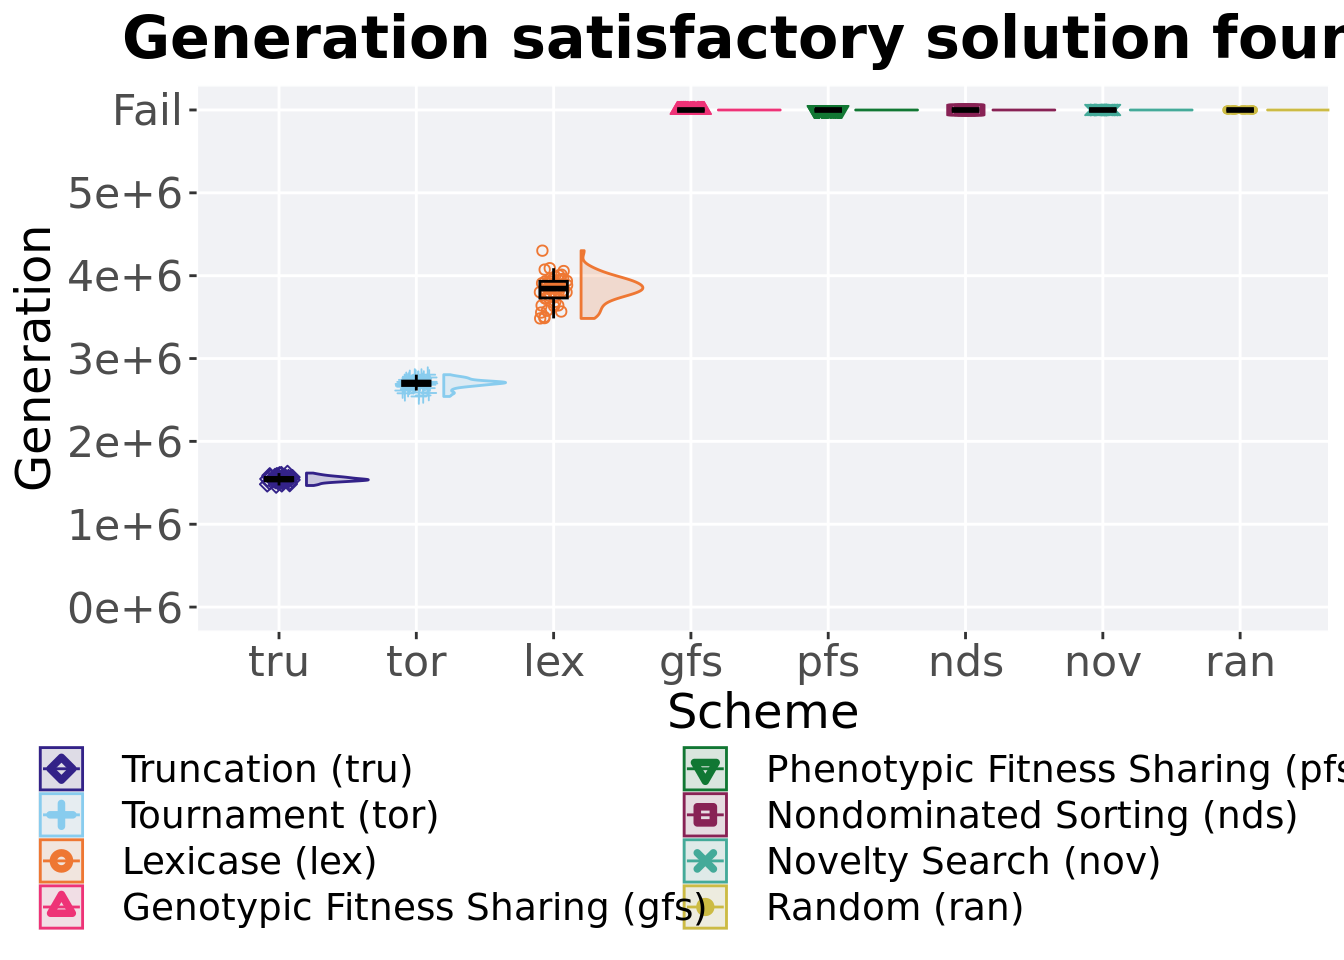
\includegraphics{demo_files/figure-latex/ord-ssf-1.pdf}

\hypertarget{stats-5}{%
\subsection{Stats}\label{stats-5}}

Summary statistics for the first generation a satisfactory solution is found throughout the 50,000 generations.

\begin{Shaded}
\begin{Highlighting}[]
\CommentTok{### Generation satisfactory solution found}
\NormalTok{ssf =}\StringTok{ }\KeywordTok{filter}\NormalTok{(cc_ssf, diagnostic }\OperatorTok{==}\StringTok{ 'ordered_exploitation'}  \OperatorTok{&}\StringTok{ }\NormalTok{Generations }\OperatorTok{<}\StringTok{ }\DecValTok{60000}\NormalTok{)}
\NormalTok{ssf}\OperatorTok{$}\NormalTok{acron =}\StringTok{ }\KeywordTok{factor}\NormalTok{(ssf}\OperatorTok{$}\NormalTok{acron, }\DataTypeTok{levels =} \KeywordTok{c}\NormalTok{(}\StringTok{'tru'}\NormalTok{, }\StringTok{'tor'}\NormalTok{, }\StringTok{'lex'}\NormalTok{))}
\NormalTok{ssf }\OperatorTok
\StringTok{  }\KeywordTok{group_by}\NormalTok{(acron) }\OperatorTok
\StringTok{  }\NormalTok{dplyr}\OperatorTok{::}\KeywordTok{summarise}\NormalTok{(}
    \DataTypeTok{count =} \KeywordTok{n}\NormalTok{(),}
    \DataTypeTok{na_cnt =} \KeywordTok{sum}\NormalTok{(}\KeywordTok{is.na}\NormalTok{(Generations)),}
    \DataTypeTok{min =} \KeywordTok{min}\NormalTok{(Generations, }\DataTypeTok{na.rm =} \OtherTok{TRUE}\NormalTok{),}
    \DataTypeTok{median =} \KeywordTok{median}\NormalTok{(Generations, }\DataTypeTok{na.rm =} \OtherTok{TRUE}\NormalTok{),}
    \DataTypeTok{mean =} \KeywordTok{mean}\NormalTok{(Generations, }\DataTypeTok{na.rm =} \OtherTok{TRUE}\NormalTok{),}
    \DataTypeTok{max =} \KeywordTok{max}\NormalTok{(Generations, }\DataTypeTok{na.rm =} \OtherTok{TRUE}\NormalTok{),}
    \DataTypeTok{IQR =} \KeywordTok{IQR}\NormalTok{(Generations, }\DataTypeTok{na.rm =} \OtherTok{TRUE}\NormalTok{)}
\NormalTok{  )}
\end{Highlighting}
\end{Shaded}

\begin{verbatim}
## # A tibble: 3 x 8
##   acron count na_cnt   min median   mean   max   IQR
##   <fct> <int>  <int> <int>  <dbl>  <dbl> <int> <dbl>
## 1 tru      50      0 14701 15466. 15511. 16280  422.
## 2 tor      50      0 25563 27254. 27122. 28151  714 
## 3 lex      50      0 35240 38918. 38865. 43751 2316.
\end{verbatim}

Kruskal--Wallis test provides evidence of difference amoung selection schemes.

\begin{Shaded}
\begin{Highlighting}[]
\KeywordTok{kruskal.test}\NormalTok{(Generations }\OperatorTok{~}\StringTok{ }\NormalTok{acron, }\DataTypeTok{data =}\NormalTok{ ssf)}
\end{Highlighting}
\end{Shaded}

\begin{verbatim}
## 
##  Kruskal-Wallis rank sum test
## 
## data:  Generations by acron
## Kruskal-Wallis chi-squared = 132.45, df = 2, p-value < 2.2e-16
\end{verbatim}

Results for post-hoc Wilcoxon rank-sum test with a Bonferroni correction.

\begin{Shaded}
\begin{Highlighting}[]
\KeywordTok{pairwise.wilcox.test}\NormalTok{(}\DataTypeTok{x =}\NormalTok{ ssf}\OperatorTok{$}\NormalTok{Generations, }\DataTypeTok{g =}\NormalTok{ ssf}\OperatorTok{$}\NormalTok{acron, }\DataTypeTok{p.adjust.method =} \StringTok{"bonferroni"}\NormalTok{,}
                     \DataTypeTok{paired =} \OtherTok{FALSE}\NormalTok{, }\DataTypeTok{conf.int =} \OtherTok{FALSE}\NormalTok{, }\DataTypeTok{alternative =} \StringTok{'g'}\NormalTok{)}
\end{Highlighting}
\end{Shaded}

\begin{verbatim}
## 
##  Pairwise comparisons using Wilcoxon rank sum test with continuity correction 
## 
## data:  ssf$Generations and ssf$acron 
## 
##     tru    tor   
## tor <2e-16 -     
## lex <2e-16 <2e-16
## 
## P value adjustment method: bonferroni
\end{verbatim}

\hypertarget{multi-valley-crossing-results-1}{%
\section{Multi-valley crossing results}\label{multi-valley-crossing-results-1}}

\hypertarget{performance-over-time-3}{%
\subsection{Performance over time}\label{performance-over-time-3}}

Best performance in a population over time.

\begin{Shaded}
\begin{Highlighting}[]
\CommentTok{# data for lines and shading on plots}
\NormalTok{lines =}\StringTok{ }\KeywordTok{filter}\NormalTok{(cc_over_time_mvc, diagnostic }\OperatorTok{==}\StringTok{ 'ordered_exploitation'}\NormalTok{) }\OperatorTok
\StringTok{  }\KeywordTok{group_by}\NormalTok{(}\StringTok{`}\DataTypeTok{Selection}\CharTok{\textbackslash{}n}\DataTypeTok{Scheme}\StringTok{`}\NormalTok{, gen) }\OperatorTok
\StringTok{  }\NormalTok{dplyr}\OperatorTok{::}\KeywordTok{summarise}\NormalTok{(}
    \DataTypeTok{min =} \KeywordTok{min}\NormalTok{(pop_fit_max) }\OperatorTok{/}\StringTok{ }\NormalTok{DIMENSIONALITY,}
    \DataTypeTok{mean =} \KeywordTok{mean}\NormalTok{(pop_fit_max) }\OperatorTok{/}\StringTok{ }\NormalTok{DIMENSIONALITY,}
    \DataTypeTok{max =} \KeywordTok{max}\NormalTok{(pop_fit_max) }\OperatorTok{/}\StringTok{ }\NormalTok{DIMENSIONALITY}
\NormalTok{  )}
\end{Highlighting}
\end{Shaded}

\begin{verbatim}
## `summarise()` has grouped output by 'Selection Scheme'. You can override using
## the `.groups` argument.
\end{verbatim}

\begin{Shaded}
\begin{Highlighting}[]
\KeywordTok{ggplot}\NormalTok{(lines, }\KeywordTok{aes}\NormalTok{(}\DataTypeTok{x=}\NormalTok{gen, }\DataTypeTok{y=}\NormalTok{mean, }\DataTypeTok{group =} \StringTok{`}\DataTypeTok{Selection}\CharTok{\textbackslash{}n}\DataTypeTok{Scheme}\StringTok{`}\NormalTok{, }\DataTypeTok{fill =}\StringTok{`}\DataTypeTok{Selection}\CharTok{\textbackslash{}n}\DataTypeTok{Scheme}\StringTok{`}\NormalTok{, }\DataTypeTok{color =} \StringTok{`}\DataTypeTok{Selection}\CharTok{\textbackslash{}n}\DataTypeTok{Scheme}\StringTok{`}\NormalTok{, }\DataTypeTok{shape =} \StringTok{`}\DataTypeTok{Selection}\CharTok{\textbackslash{}n}\DataTypeTok{Scheme}\StringTok{`}\NormalTok{)) }\OperatorTok{+}
\StringTok{  }\KeywordTok{geom_ribbon}\NormalTok{(}\KeywordTok{aes}\NormalTok{(}\DataTypeTok{ymin =}\NormalTok{ min, }\DataTypeTok{ymax =}\NormalTok{ max), }\DataTypeTok{alpha =} \FloatTok{0.1}\NormalTok{) }\OperatorTok{+}
\StringTok{  }\KeywordTok{geom_line}\NormalTok{(}\DataTypeTok{size =} \FloatTok{0.5}\NormalTok{) }\OperatorTok{+}
\StringTok{  }\KeywordTok{geom_point}\NormalTok{(}\DataTypeTok{data =} \KeywordTok{filter}\NormalTok{(lines, gen }\OperatorTok\StringTok{ }\DecValTok{2000} \OperatorTok{==}\StringTok{ }\DecValTok{0} \OperatorTok{&}\StringTok{ }\NormalTok{gen }\OperatorTok{!=}\StringTok{ }\DecValTok{0}\NormalTok{), }\DataTypeTok{size =} \FloatTok{1.5}\NormalTok{, }\DataTypeTok{stroke =} \FloatTok{2.0}\NormalTok{, }\DataTypeTok{alpha =} \FloatTok{1.0}\NormalTok{) }\OperatorTok{+}
\StringTok{  }\KeywordTok{scale_y_continuous}\NormalTok{(}
    \DataTypeTok{name=}\StringTok{"Average trait score"}\NormalTok{,}
    \DataTypeTok{limits=}\KeywordTok{c}\NormalTok{(}\DecValTok{0}\NormalTok{, }\DecValTok{15}\NormalTok{),}
    \DataTypeTok{breaks=}\KeywordTok{seq}\NormalTok{(}\DecValTok{0}\NormalTok{,}\DecValTok{15}\NormalTok{, }\DecValTok{5}\NormalTok{),}
    \DataTypeTok{labels=}\KeywordTok{c}\NormalTok{(}\StringTok{"0"}\NormalTok{, }\StringTok{"5"}\NormalTok{, }\StringTok{"10"}\NormalTok{, }\StringTok{"15"}\NormalTok{)}
\NormalTok{  ) }\OperatorTok{+}
\StringTok{  }\KeywordTok{scale_x_continuous}\NormalTok{(}
    \DataTypeTok{name=}\StringTok{"Generations"}\NormalTok{,}
    \DataTypeTok{limits=}\KeywordTok{c}\NormalTok{(}\DecValTok{0}\NormalTok{, }\DecValTok{50000}\NormalTok{),}
    \DataTypeTok{breaks=}\KeywordTok{c}\NormalTok{(}\DecValTok{0}\NormalTok{, }\DecValTok{10000}\NormalTok{, }\DecValTok{20000}\NormalTok{, }\DecValTok{30000}\NormalTok{, }\DecValTok{40000}\NormalTok{, }\DecValTok{50000}\NormalTok{),}
    \DataTypeTok{labels=}\KeywordTok{c}\NormalTok{(}\StringTok{"0e+4"}\NormalTok{, }\StringTok{"1e+4"}\NormalTok{, }\StringTok{"2e+4"}\NormalTok{, }\StringTok{"3e+4"}\NormalTok{, }\StringTok{"4e+4"}\NormalTok{, }\StringTok{"5e+4"}\NormalTok{)}

\NormalTok{  ) }\OperatorTok{+}
\StringTok{  }\KeywordTok{scale_shape_manual}\NormalTok{(}\DataTypeTok{values=}\NormalTok{SHAPE)}\OperatorTok{+}
\StringTok{  }\KeywordTok{scale_colour_manual}\NormalTok{(}\DataTypeTok{values =}\NormalTok{ cb_palette) }\OperatorTok{+}
\StringTok{  }\KeywordTok{scale_fill_manual}\NormalTok{(}\DataTypeTok{values =}\NormalTok{ cb_palette) }\OperatorTok{+}
\StringTok{  }\KeywordTok{ggtitle}\NormalTok{(}\StringTok{'Performance over time'}\NormalTok{)}\OperatorTok{+}
\StringTok{  }\NormalTok{p_theme }\OperatorTok{+}\StringTok{ }\KeywordTok{theme}\NormalTok{(}\DataTypeTok{legend.title=}\KeywordTok{element_blank}\NormalTok{(),}\DataTypeTok{legend.text=}\KeywordTok{element_text}\NormalTok{(}\DataTypeTok{size=}\DecValTok{12}\NormalTok{)) }\OperatorTok{+}
\StringTok{  }\KeywordTok{guides}\NormalTok{(}
    \DataTypeTok{shape=}\KeywordTok{guide_legend}\NormalTok{(}\DataTypeTok{ncol=}\DecValTok{2}\NormalTok{, }\DataTypeTok{title.position =} \StringTok{"left"}\NormalTok{),}
    \DataTypeTok{color=}\KeywordTok{guide_legend}\NormalTok{(}\DataTypeTok{ncol=}\DecValTok{2}\NormalTok{, }\DataTypeTok{title.position =} \StringTok{"left"}\NormalTok{),}
    \DataTypeTok{fill=}\KeywordTok{guide_legend}\NormalTok{(}\DataTypeTok{ncol=}\DecValTok{2}\NormalTok{, }\DataTypeTok{title.position =} \StringTok{"left"}\NormalTok{)}
\NormalTok{  )}
\end{Highlighting}
\end{Shaded}

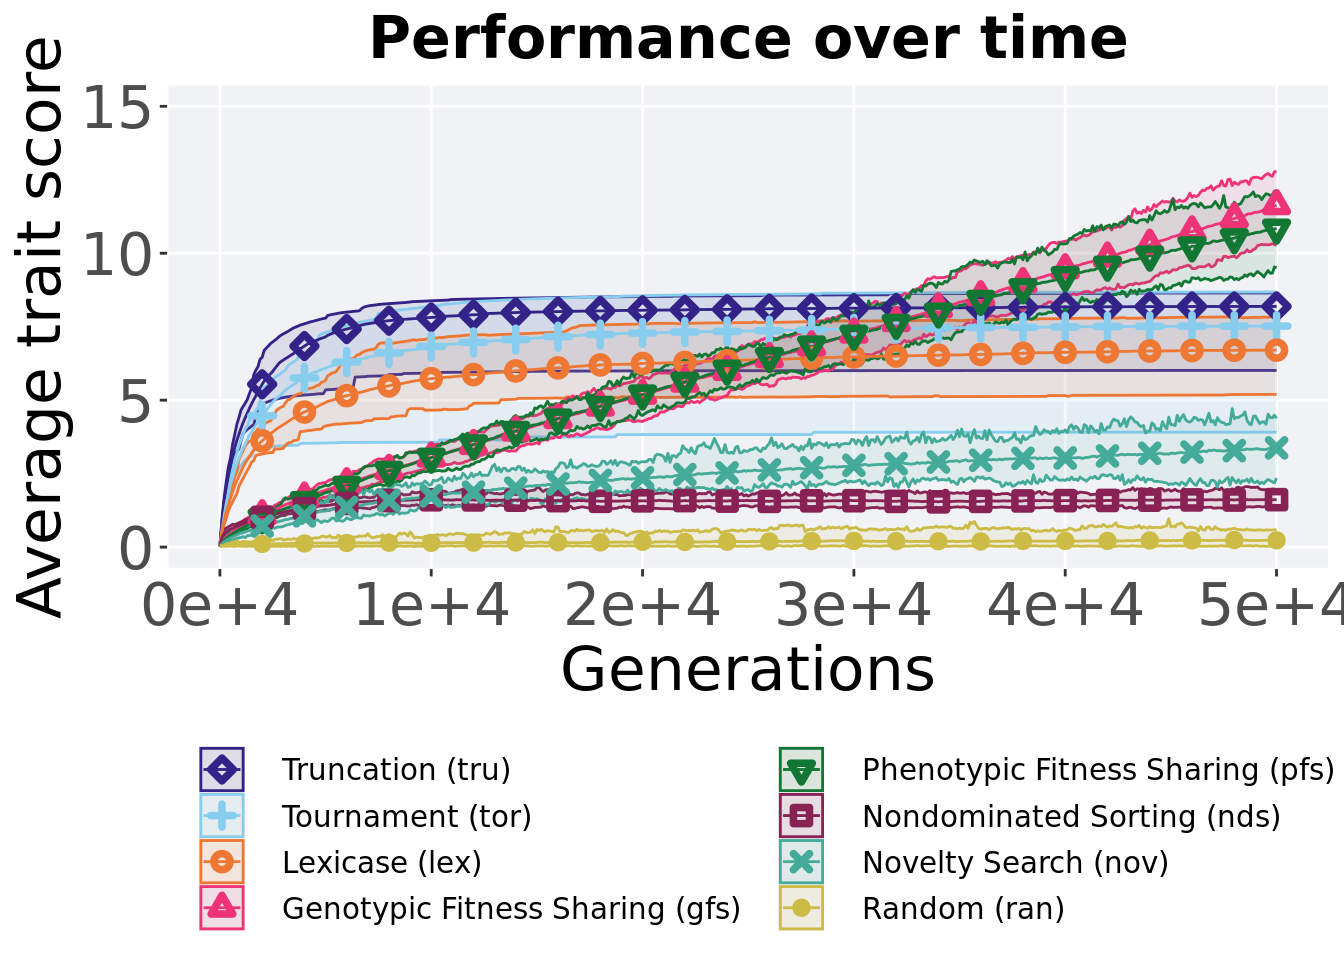
\includegraphics{demo_files/figure-latex/ord-mvc-per-ot-1.pdf}

\hypertarget{best-performance-throughout-3}{%
\subsection{Best performance throughout}\label{best-performance-throughout-3}}

Best performance found throughout 50,000 generations.

\begin{Shaded}
\begin{Highlighting}[]
\CommentTok{### best performance throughout}
\KeywordTok{filter}\NormalTok{(cc_best_mvc, col }\OperatorTok{==}\StringTok{ 'pop_fit_max'} \OperatorTok{&}\StringTok{ }\NormalTok{diagnostic }\OperatorTok{==}\StringTok{ 'ordered_exploitation'}\NormalTok{) }\OperatorTok
\StringTok{  }\KeywordTok{ggplot}\NormalTok{(., }\KeywordTok{aes}\NormalTok{(}\DataTypeTok{x =}\NormalTok{ acron, }\DataTypeTok{y =}\NormalTok{ val }\OperatorTok{/}\StringTok{ }\NormalTok{DIMENSIONALITY, }\DataTypeTok{color =}\NormalTok{ acron, }\DataTypeTok{fill =}\NormalTok{ acron, }\DataTypeTok{shape =}\NormalTok{ acron)) }\OperatorTok{+}
\StringTok{  }\KeywordTok{geom_flat_violin}\NormalTok{(}\DataTypeTok{position =} \KeywordTok{position_nudge}\NormalTok{(}\DataTypeTok{x =} \FloatTok{.2}\NormalTok{, }\DataTypeTok{y =} \DecValTok{0}\NormalTok{), }\DataTypeTok{scale =} \StringTok{'width'}\NormalTok{, }\DataTypeTok{alpha =} \FloatTok{0.2}\NormalTok{) }\OperatorTok{+}
\StringTok{  }\KeywordTok{geom_point}\NormalTok{(}\DataTypeTok{position =} \KeywordTok{position_jitter}\NormalTok{(}\DataTypeTok{width =} \FloatTok{.1}\NormalTok{), }\DataTypeTok{size =} \FloatTok{1.5}\NormalTok{, }\DataTypeTok{alpha =} \FloatTok{1.0}\NormalTok{) }\OperatorTok{+}
\StringTok{  }\KeywordTok{geom_boxplot}\NormalTok{(}\DataTypeTok{color =} \StringTok{'black'}\NormalTok{, }\DataTypeTok{width =} \FloatTok{.2}\NormalTok{, }\DataTypeTok{outlier.shape =} \OtherTok{NA}\NormalTok{, }\DataTypeTok{alpha =} \FloatTok{0.0}\NormalTok{) }\OperatorTok{+}
\StringTok{  }\KeywordTok{guides}\NormalTok{(}\DataTypeTok{fill =} \StringTok{"none"}\NormalTok{,}\DataTypeTok{color =} \StringTok{'none'}\NormalTok{, }\DataTypeTok{shape =} \StringTok{'none'}\NormalTok{) }\OperatorTok{+}
\StringTok{  }\KeywordTok{scale_y_continuous}\NormalTok{(}
    \DataTypeTok{name=}\StringTok{"Average trait score"}\NormalTok{,}
    \DataTypeTok{limits=}\KeywordTok{c}\NormalTok{(}\DecValTok{0}\NormalTok{, }\DecValTok{15}\NormalTok{),}
    \DataTypeTok{breaks=}\KeywordTok{seq}\NormalTok{(}\DecValTok{0}\NormalTok{,}\DecValTok{15}\NormalTok{, }\DecValTok{5}\NormalTok{),}
    \DataTypeTok{labels=}\KeywordTok{c}\NormalTok{(}\StringTok{"0"}\NormalTok{, }\StringTok{"5"}\NormalTok{, }\StringTok{"10"}\NormalTok{, }\StringTok{"15"}\NormalTok{)}
\NormalTok{  ) }\OperatorTok{+}
\StringTok{  }\KeywordTok{scale_x_discrete}\NormalTok{(}
    \DataTypeTok{name=}\StringTok{"Scheme"}
\NormalTok{  )}\OperatorTok{+}
\StringTok{  }\KeywordTok{scale_shape_manual}\NormalTok{(}\DataTypeTok{values=}\NormalTok{SHAPE)}\OperatorTok{+}
\StringTok{  }\KeywordTok{scale_colour_manual}\NormalTok{(}\DataTypeTok{values =}\NormalTok{ cb_palette, ) }\OperatorTok{+}
\StringTok{  }\KeywordTok{scale_fill_manual}\NormalTok{(}\DataTypeTok{values =}\NormalTok{ cb_palette) }\OperatorTok{+}
\StringTok{  }\KeywordTok{ggtitle}\NormalTok{(}\StringTok{'Best performance throughout'}\NormalTok{)}\OperatorTok{+}
\StringTok{  }\NormalTok{p_theme }\OperatorTok{+}\StringTok{ }\KeywordTok{theme}\NormalTok{(}\DataTypeTok{legend.title=}\KeywordTok{element_blank}\NormalTok{()) }\OperatorTok{+}
\StringTok{  }\KeywordTok{guides}\NormalTok{(}
    \DataTypeTok{shape=}\KeywordTok{guide_legend}\NormalTok{(}\DataTypeTok{nrow=}\DecValTok{2}\NormalTok{, }\DataTypeTok{title.position =} \StringTok{"bottom"}\NormalTok{),}
    \DataTypeTok{color=}\KeywordTok{guide_legend}\NormalTok{(}\DataTypeTok{nrow=}\DecValTok{2}\NormalTok{, }\DataTypeTok{title.position =} \StringTok{"bottom"}\NormalTok{),}
    \DataTypeTok{fill=}\KeywordTok{guide_legend}\NormalTok{(}\DataTypeTok{nrow=}\DecValTok{2}\NormalTok{, }\DataTypeTok{title.position =} \StringTok{"bottom"}\NormalTok{)}
\NormalTok{  )}
\end{Highlighting}
\end{Shaded}

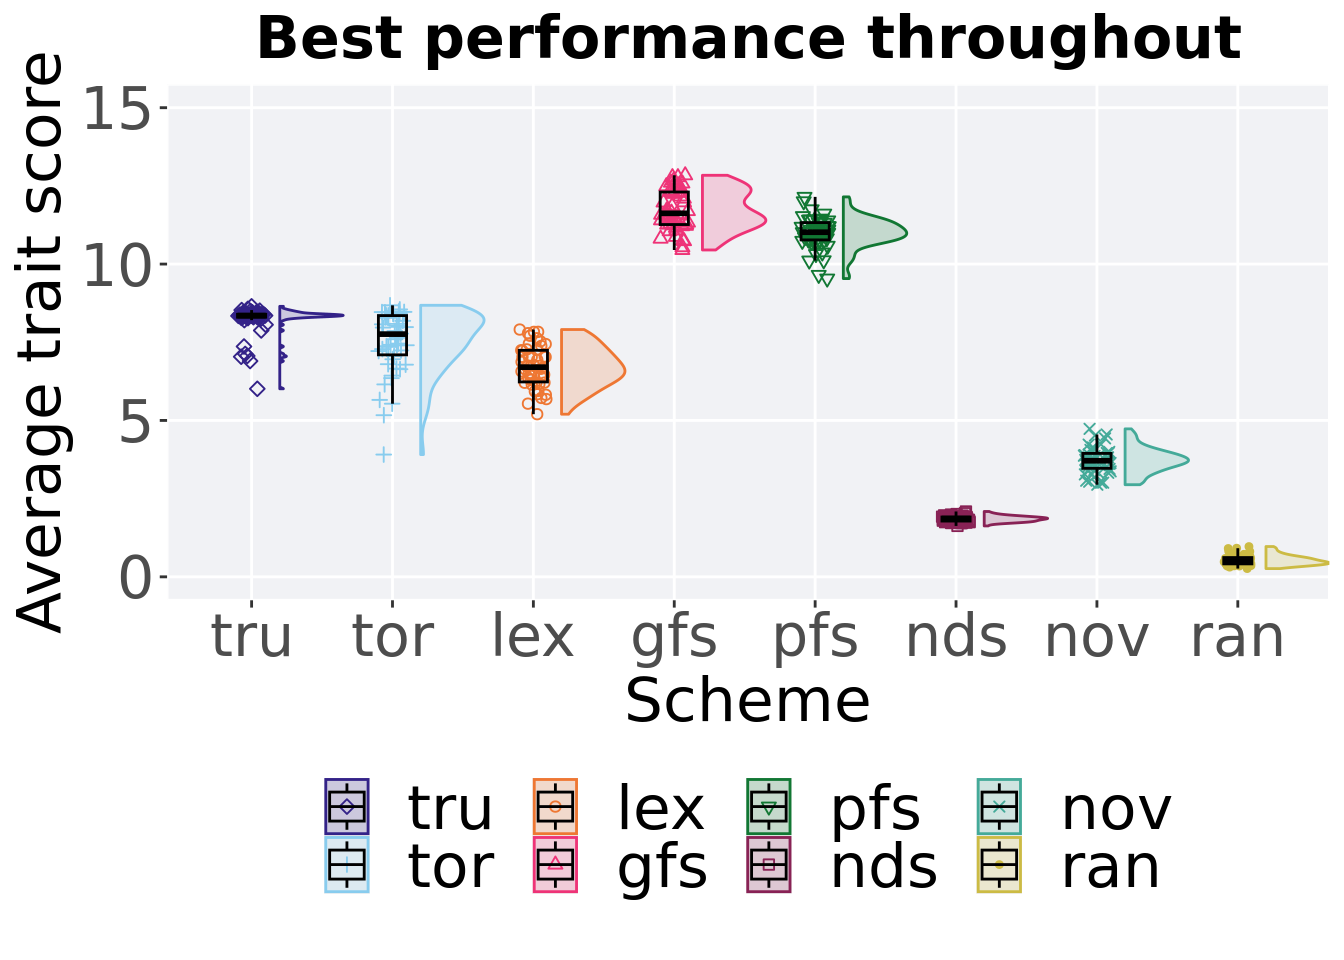
\includegraphics{demo_files/figure-latex/ord-mvc-per-bst-1.pdf}

\hypertarget{stats-6}{%
\subsubsection{Stats}\label{stats-6}}

Summary statistics for the performance of the best performance.

\begin{Shaded}
\begin{Highlighting}[]
\CommentTok{#get data & summarize}
\NormalTok{performance =}\StringTok{ }\KeywordTok{filter}\NormalTok{(cc_best_mvc, col }\OperatorTok{==}\StringTok{ 'pop_fit_max'} \OperatorTok{&}\StringTok{ }\NormalTok{diagnostic }\OperatorTok{==}\StringTok{ 'ordered_exploitation'}\NormalTok{)}
\NormalTok{performance}\OperatorTok{$}\NormalTok{acron =}\StringTok{ }\KeywordTok{factor}\NormalTok{(performance}\OperatorTok{$}\NormalTok{acron, }\DataTypeTok{levels =} \KeywordTok{c}\NormalTok{(}\StringTok{'gfs'}\NormalTok{,}\StringTok{'pfs'}\NormalTok{,}\StringTok{'tru'}\NormalTok{,}\StringTok{'tor'}\NormalTok{,}\StringTok{'lex'}\NormalTok{,}\StringTok{'nov'}\NormalTok{, }\StringTok{'nds'}\NormalTok{, }\StringTok{'ran'}\NormalTok{))}
\NormalTok{performance }\OperatorTok
\StringTok{  }\KeywordTok{group_by}\NormalTok{(acron) }\OperatorTok
\StringTok{  }\NormalTok{dplyr}\OperatorTok{::}\KeywordTok{summarise}\NormalTok{(}
    \DataTypeTok{count =} \KeywordTok{n}\NormalTok{(),}
    \DataTypeTok{na_cnt =} \KeywordTok{sum}\NormalTok{(}\KeywordTok{is.na}\NormalTok{(val)),}
    \DataTypeTok{min =} \KeywordTok{min}\NormalTok{(val }\OperatorTok{/}\StringTok{ }\NormalTok{DIMENSIONALITY, }\DataTypeTok{na.rm =} \OtherTok{TRUE}\NormalTok{),}
    \DataTypeTok{median =} \KeywordTok{median}\NormalTok{(val }\OperatorTok{/}\StringTok{ }\NormalTok{DIMENSIONALITY, }\DataTypeTok{na.rm =} \OtherTok{TRUE}\NormalTok{),}
    \DataTypeTok{mean =} \KeywordTok{mean}\NormalTok{(val }\OperatorTok{/}\StringTok{ }\NormalTok{DIMENSIONALITY, }\DataTypeTok{na.rm =} \OtherTok{TRUE}\NormalTok{),}
    \DataTypeTok{max =} \KeywordTok{max}\NormalTok{(val }\OperatorTok{/}\StringTok{ }\NormalTok{DIMENSIONALITY, }\DataTypeTok{na.rm =} \OtherTok{TRUE}\NormalTok{),}
    \DataTypeTok{IQR =} \KeywordTok{IQR}\NormalTok{(val }\OperatorTok{/}\StringTok{ }\NormalTok{DIMENSIONALITY, }\DataTypeTok{na.rm =} \OtherTok{TRUE}\NormalTok{)}
\NormalTok{  )}
\end{Highlighting}
\end{Shaded}

\begin{verbatim}
## # A tibble: 8 x 8
##   acron count na_cnt    min median   mean    max    IQR
##   <fct> <int>  <int>  <dbl>  <dbl>  <dbl>  <dbl>  <dbl>
## 1 gfs      50      0 10.5   11.6   11.7   12.8   1.04  
## 2 pfs      50      0  9.54  11.0   11.0   12.1   0.553 
## 3 tru      50      0  6.01   8.35   8.19   8.65  0.0922
## 4 tor      50      0  3.91   7.76   7.52   8.68  1.26  
## 5 lex      50      0  5.20   6.70   6.72   7.91  1.01  
## 6 nov      50      0  2.95   3.71   3.72   4.73  0.476 
## 7 nds      50      0  1.63   1.86   1.85   2.09  0.129 
## 8 ran      50      0  0.263  0.490  0.534  0.968 0.202
\end{verbatim}

Kruskal--Wallis test provides evidence of statistical differences.

\begin{Shaded}
\begin{Highlighting}[]
\KeywordTok{kruskal.test}\NormalTok{(val }\OperatorTok{~}\StringTok{ }\NormalTok{acron, }\DataTypeTok{data =}\NormalTok{ performance)}
\end{Highlighting}
\end{Shaded}

\begin{verbatim}
## 
##  Kruskal-Wallis rank sum test
## 
## data:  val by acron
## Kruskal-Wallis chi-squared = 380.23, df = 7, p-value < 2.2e-16
\end{verbatim}

Results for post-hoc Wilcoxon rank-sum test with a Bonferroni correction.

\begin{Shaded}
\begin{Highlighting}[]
\KeywordTok{pairwise.wilcox.test}\NormalTok{(}\DataTypeTok{x =}\NormalTok{ performance}\OperatorTok{$}\NormalTok{val, }\DataTypeTok{g =}\NormalTok{ performance}\OperatorTok{$}\NormalTok{acron, }\DataTypeTok{p.adjust.method =} \StringTok{"bonferroni"}\NormalTok{,}
                     \DataTypeTok{paired =} \OtherTok{FALSE}\NormalTok{, }\DataTypeTok{conf.int =} \OtherTok{FALSE}\NormalTok{, }\DataTypeTok{alternative =} \StringTok{'l'}\NormalTok{)}
\end{Highlighting}
\end{Shaded}

\begin{verbatim}
## 
##  Pairwise comparisons using Wilcoxon rank sum test with continuity correction 
## 
## data:  performance$val and performance$acron 
## 
##     gfs     pfs     tru     tor     lex     nov     nds    
## pfs 1.6e-06 -       -       -       -       -       -      
## tru < 2e-16 < 2e-16 -       -       -       -       -      
## tor < 2e-16 < 2e-16 0.0026  -       -       -       -      
## lex < 2e-16 < 2e-16 7.7e-14 1.7e-05 -       -       -      
## nov < 2e-16 < 2e-16 < 2e-16 2.4e-16 < 2e-16 -       -      
## nds < 2e-16 < 2e-16 < 2e-16 < 2e-16 < 2e-16 < 2e-16 -      
## ran < 2e-16 < 2e-16 < 2e-16 < 2e-16 < 2e-16 < 2e-16 < 2e-16
## 
## P value adjustment method: bonferroni
\end{verbatim}

\hypertarget{performance-comparison-1}{%
\subsection{Performance comparison}\label{performance-comparison-1}}

Best performances in the population at 40,000 and 50,000 generations.

\begin{verbatim}
## Warning: The following aesthetics were dropped during statistical transformation:
## colour, shape
## i This can happen when ggplot fails to infer the correct grouping structure in
##   the data.
## i Did you forget to specify a `group` aesthetic or to convert a numerical
##   variable into a factor?
## The following aesthetics were dropped during statistical transformation:
## colour, shape
## i This can happen when ggplot fails to infer the correct grouping structure in
##   the data.
## i Did you forget to specify a `group` aesthetic or to convert a numerical
##   variable into a factor?
\end{verbatim}

\begin{Shaded}
\begin{Highlighting}[]
\CommentTok{# 80% and final generation comparison}
\NormalTok{end =}\StringTok{ }\KeywordTok{filter}\NormalTok{(cc_over_time_mvc, diagnostic }\OperatorTok{==}\StringTok{ 'ordered_exploitation'} \OperatorTok{&}\StringTok{ }\NormalTok{gen }\OperatorTok{==}\StringTok{ }\DecValTok{50000} \OperatorTok{&}\StringTok{ }\NormalTok{acron }\OperatorTok{!=}\StringTok{ 'ran'}\NormalTok{)}
\NormalTok{end}\OperatorTok{$}\NormalTok{Generation <-}\StringTok{ }\KeywordTok{factor}\NormalTok{(end}\OperatorTok{$}\NormalTok{gen)}

\NormalTok{mid =}\StringTok{ }\KeywordTok{filter}\NormalTok{(cc_over_time_mvc, diagnostic }\OperatorTok{==}\StringTok{ 'ordered_exploitation'} \OperatorTok{&}\StringTok{ }\NormalTok{gen }\OperatorTok{==}\StringTok{ }\DecValTok{40000} \OperatorTok{&}\StringTok{ }\NormalTok{acron }\OperatorTok{!=}\StringTok{ 'ran'}\NormalTok{)}
\NormalTok{mid}\OperatorTok{$}\NormalTok{Generation <-}\StringTok{ }\KeywordTok{factor}\NormalTok{(mid}\OperatorTok{$}\NormalTok{gen)}

\NormalTok{mvc_p =}\StringTok{ }\KeywordTok{ggplot}\NormalTok{(mid, }\KeywordTok{aes}\NormalTok{(}\DataTypeTok{x =}\NormalTok{ acron, }\DataTypeTok{y=}\NormalTok{pop_fit_max }\OperatorTok{/}\StringTok{ }\NormalTok{DIMENSIONALITY, }\DataTypeTok{group =}\NormalTok{ acron, }\DataTypeTok{shape =}\NormalTok{ Generation)) }\OperatorTok{+}
\StringTok{  }\KeywordTok{geom_point}\NormalTok{(}\DataTypeTok{col =}\NormalTok{ mvc_col[}\DecValTok{1}\NormalTok{] , }\DataTypeTok{position =} \KeywordTok{position_jitternudge}\NormalTok{(}\DataTypeTok{jitter.width =} \FloatTok{.03}\NormalTok{, }\DataTypeTok{nudge.x =} \FloatTok{-0.05}\NormalTok{), }\DataTypeTok{size =} \DecValTok{2}\NormalTok{, }\DataTypeTok{alpha =} \FloatTok{1.0}\NormalTok{) }\OperatorTok{+}
\StringTok{  }\KeywordTok{geom_boxplot}\NormalTok{(}\DataTypeTok{position =} \KeywordTok{position_nudge}\NormalTok{(}\DataTypeTok{x =} \FloatTok{-.15}\NormalTok{, }\DataTypeTok{y =} \DecValTok{0}\NormalTok{), }\DataTypeTok{lwd =} \FloatTok{0.7}\NormalTok{, }\DataTypeTok{col =}\NormalTok{ mvc_col[}\DecValTok{1}\NormalTok{], }\DataTypeTok{fill =}\NormalTok{ mvc_col[}\DecValTok{1}\NormalTok{], }\DataTypeTok{width =} \FloatTok{.1}\NormalTok{, }\DataTypeTok{outlier.shape =} \OtherTok{NA}\NormalTok{, }\DataTypeTok{alpha =} \FloatTok{0.0}\NormalTok{) }\OperatorTok{+}

\StringTok{  }\KeywordTok{geom_point}\NormalTok{(}\DataTypeTok{data =}\NormalTok{ end, }\KeywordTok{aes}\NormalTok{(}\DataTypeTok{x =}\NormalTok{ acron, }\DataTypeTok{y=}\NormalTok{pop_fit_max }\OperatorTok{/}\StringTok{ }\NormalTok{DIMENSIONALITY), }\DataTypeTok{col =}\NormalTok{ mvc_col[}\DecValTok{2}\NormalTok{], }\DataTypeTok{position =} \KeywordTok{position_jitternudge}\NormalTok{(}\DataTypeTok{jitter.width =} \FloatTok{.03}\NormalTok{, }\DataTypeTok{nudge.x =} \FloatTok{0.05}\NormalTok{), }\DataTypeTok{size =} \DecValTok{2}\NormalTok{, }\DataTypeTok{alpha =} \FloatTok{1.0}\NormalTok{) }\OperatorTok{+}
\StringTok{  }\KeywordTok{geom_boxplot}\NormalTok{(}\DataTypeTok{data =}\NormalTok{ end, }\KeywordTok{aes}\NormalTok{(}\DataTypeTok{x =}\NormalTok{ acron, }\DataTypeTok{y=}\NormalTok{pop_fit_max }\OperatorTok{/}\StringTok{ }\NormalTok{DIMENSIONALITY), }\DataTypeTok{position =} \KeywordTok{position_nudge}\NormalTok{(}\DataTypeTok{x =} \FloatTok{.15}\NormalTok{, }\DataTypeTok{y =} \DecValTok{0}\NormalTok{), }\DataTypeTok{lwd =} \FloatTok{0.7}\NormalTok{, }\DataTypeTok{col =}\NormalTok{ mvc_col[}\DecValTok{2}\NormalTok{], }\DataTypeTok{fill =}\NormalTok{ mvc_col[}\DecValTok{2}\NormalTok{], }\DataTypeTok{width =} \FloatTok{.1}\NormalTok{, }\DataTypeTok{outlier.shape =} \OtherTok{NA}\NormalTok{, }\DataTypeTok{alpha =} \FloatTok{0.0}\NormalTok{) }\OperatorTok{+}

\StringTok{  }\KeywordTok{scale_y_continuous}\NormalTok{(}
    \DataTypeTok{name=}\StringTok{"Average trait score"}\NormalTok{,}
    \DataTypeTok{limits=}\KeywordTok{c}\NormalTok{(}\DecValTok{0}\NormalTok{, }\DecValTok{15}\NormalTok{),}
    \DataTypeTok{breaks=}\KeywordTok{seq}\NormalTok{(}\DecValTok{0}\NormalTok{,}\DecValTok{15}\NormalTok{, }\DecValTok{5}\NormalTok{),}
    \DataTypeTok{labels=}\KeywordTok{c}\NormalTok{(}\StringTok{"0"}\NormalTok{, }\StringTok{"5"}\NormalTok{, }\StringTok{"10"}\NormalTok{, }\StringTok{"15"}\NormalTok{)}
\NormalTok{  ) }\OperatorTok{+}
\StringTok{  }\KeywordTok{scale_x_discrete}\NormalTok{(}
    \DataTypeTok{name=}\StringTok{"Scheme"}
\NormalTok{  )}\OperatorTok{+}
\StringTok{  }\KeywordTok{scale_shape_manual}\NormalTok{(}\DataTypeTok{values=}\KeywordTok{c}\NormalTok{(}\DecValTok{0}\NormalTok{,}\DecValTok{1}\NormalTok{))}\OperatorTok{+}
\StringTok{  }\KeywordTok{scale_colour_manual}\NormalTok{(}\DataTypeTok{values =} \KeywordTok{c}\NormalTok{(mvc_col[}\DecValTok{1}\NormalTok{],mvc_col[}\DecValTok{2}\NormalTok{])) }\OperatorTok{+}
\StringTok{  }\NormalTok{p_theme}

\KeywordTok{plot_grid}\NormalTok{(}
\NormalTok{  mvc_p }\OperatorTok{+}
\StringTok{    }\KeywordTok{ggtitle}\NormalTok{(}\StringTok{"Performance comparisons"}\NormalTok{) }\OperatorTok{+}
\StringTok{    }\KeywordTok{theme}\NormalTok{(}\DataTypeTok{legend.position=}\StringTok{"none"}\NormalTok{),}
\NormalTok{  legend,}
  \DataTypeTok{nrow=}\DecValTok{2}\NormalTok{,}
  \DataTypeTok{rel_heights =} \KeywordTok{c}\NormalTok{(}\DecValTok{1}\NormalTok{,.}\DecValTok{05}\NormalTok{),}
  \DataTypeTok{label_size =}\NormalTok{ TSIZE}
\NormalTok{)}
\end{Highlighting}
\end{Shaded}

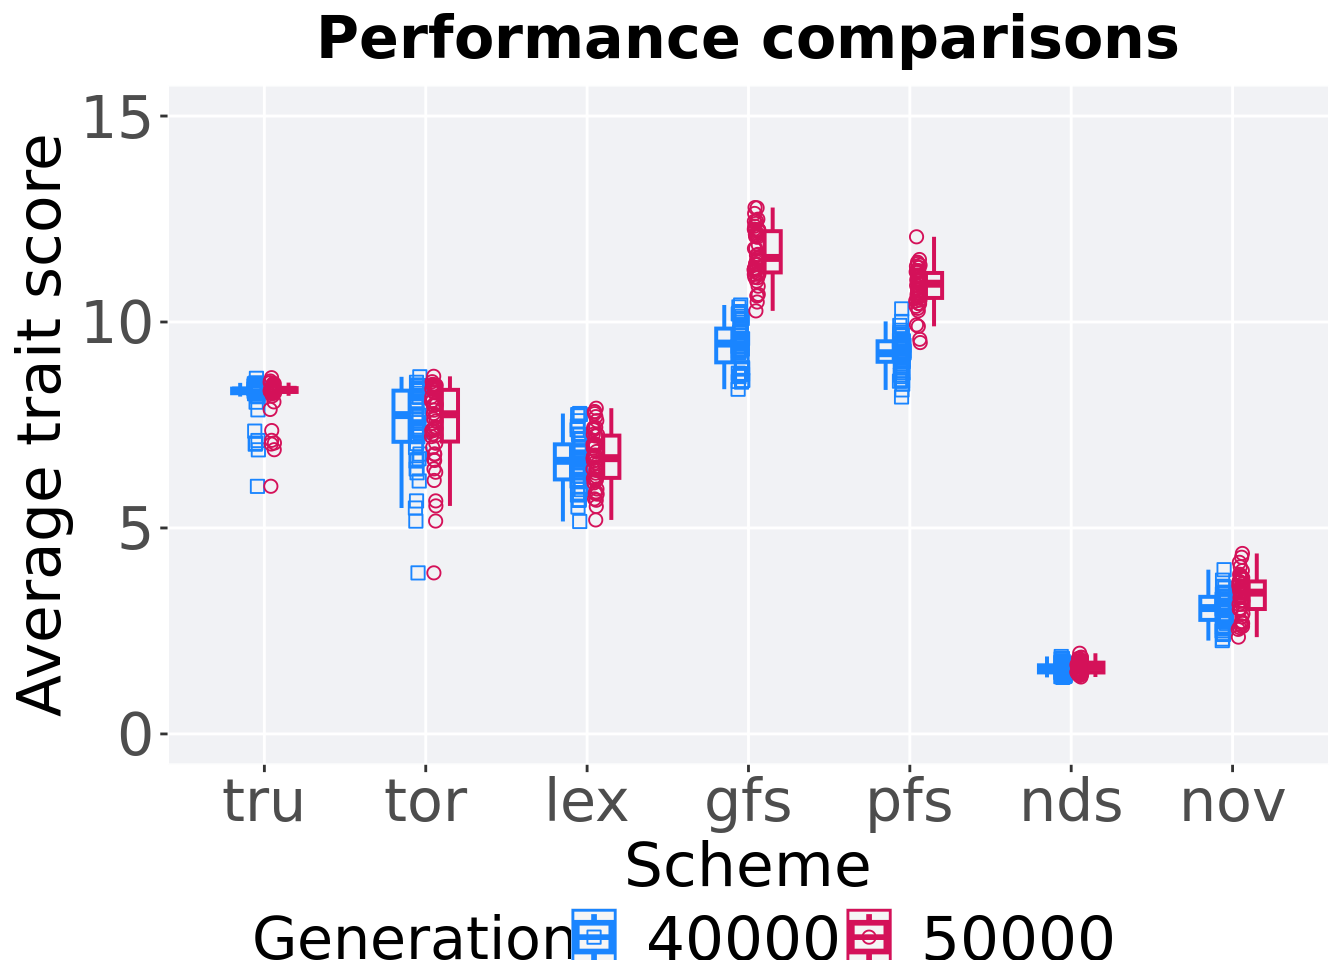
\includegraphics{demo_files/figure-latex/ord-mvc-per-sli-1.pdf}

\hypertarget{stats-7}{%
\subsubsection{Stats}\label{stats-7}}

Summary statistics for the performance of the best performance at 40,000 and 50,000 generations.

\begin{Shaded}
\begin{Highlighting}[]
\CommentTok{### performance comparisons and generation slices 40K & 50K}
\NormalTok{slices =}\StringTok{ }\KeywordTok{filter}\NormalTok{(cc_over_time_mvc, diagnostic }\OperatorTok{==}\StringTok{ 'ordered_exploitation'} \OperatorTok{&}\StringTok{ }\NormalTok{(gen }\OperatorTok{==}\StringTok{ }\DecValTok{50000} \OperatorTok{|}\StringTok{ }\NormalTok{gen }\OperatorTok{==}\StringTok{ }\DecValTok{40000}\NormalTok{) }\OperatorTok{&}\StringTok{ }\NormalTok{acron }\OperatorTok{!=}\StringTok{ 'ran'}\NormalTok{)}
\NormalTok{slices}\OperatorTok{$}\NormalTok{Generation <-}\StringTok{ }\KeywordTok{factor}\NormalTok{(slices}\OperatorTok{$}\NormalTok{gen, }\DataTypeTok{levels =} \KeywordTok{c}\NormalTok{(}\DecValTok{50000}\NormalTok{,}\DecValTok{40000}\NormalTok{))}
\NormalTok{slices}\OperatorTok{$}\NormalTok{acron =}\StringTok{ }\KeywordTok{factor}\NormalTok{(slices}\OperatorTok{$}\NormalTok{acron, }\DataTypeTok{levels =} \KeywordTok{c}\NormalTok{(}\StringTok{'gfs'}\NormalTok{,}\StringTok{'pfs'}\NormalTok{,}\StringTok{'tru'}\NormalTok{,}\StringTok{'tor'}\NormalTok{,}\StringTok{'lex'}\NormalTok{,}\StringTok{'nov'}\NormalTok{, }\StringTok{'nds'}\NormalTok{, }\StringTok{'ran'}\NormalTok{))}
\NormalTok{slices }\OperatorTok
\StringTok{  }\KeywordTok{group_by}\NormalTok{(acron, Generation) }\OperatorTok
\StringTok{  }\NormalTok{dplyr}\OperatorTok{::}\KeywordTok{summarise}\NormalTok{(}
    \DataTypeTok{count =} \KeywordTok{n}\NormalTok{(),}
    \DataTypeTok{na_cnt =} \KeywordTok{sum}\NormalTok{(}\KeywordTok{is.na}\NormalTok{(pop_fit_max  }\OperatorTok{/}\StringTok{ }\NormalTok{DIMENSIONALITY)),}
    \DataTypeTok{min =} \KeywordTok{min}\NormalTok{(pop_fit_max  }\OperatorTok{/}\StringTok{ }\NormalTok{DIMENSIONALITY, }\DataTypeTok{na.rm =} \OtherTok{TRUE}\NormalTok{),}
    \DataTypeTok{median =} \KeywordTok{median}\NormalTok{(pop_fit_max  }\OperatorTok{/}\StringTok{ }\NormalTok{DIMENSIONALITY, }\DataTypeTok{na.rm =} \OtherTok{TRUE}\NormalTok{),}
    \DataTypeTok{mean =} \KeywordTok{mean}\NormalTok{(pop_fit_max  }\OperatorTok{/}\StringTok{ }\NormalTok{DIMENSIONALITY, }\DataTypeTok{na.rm =} \OtherTok{TRUE}\NormalTok{),}
    \DataTypeTok{max =} \KeywordTok{max}\NormalTok{(pop_fit_max  }\OperatorTok{/}\StringTok{ }\NormalTok{DIMENSIONALITY, }\DataTypeTok{na.rm =} \OtherTok{TRUE}\NormalTok{),}
    \DataTypeTok{IQR =} \KeywordTok{IQR}\NormalTok{(pop_fit_max  }\OperatorTok{/}\StringTok{ }\NormalTok{DIMENSIONALITY, }\DataTypeTok{na.rm =} \OtherTok{TRUE}\NormalTok{)}
\NormalTok{  )}
\end{Highlighting}
\end{Shaded}

\begin{verbatim}
## `summarise()` has grouped output by 'acron'. You can override using the
## `.groups` argument.
\end{verbatim}

\begin{verbatim}
## # A tibble: 14 x 9
## # Groups:   acron [7]
##    acron Generation count na_cnt   min median  mean   max    IQR
##    <fct> <fct>      <int>  <int> <dbl>  <dbl> <dbl> <dbl>  <dbl>
##  1 gfs   50000         50      0 10.3   11.6  11.6  12.8  1.00  
##  2 gfs   40000         50      0  8.37   9.48  9.45 10.4  0.820 
##  3 pfs   50000         50      0  9.50  10.9  10.8  12.1  0.606 
##  4 pfs   40000         50      0  8.18   9.24  9.23 10.3  0.498 
##  5 tru   50000         50      0  6.01   8.35  8.19  8.65 0.0922
##  6 tru   40000         50      0  6.01   8.33  8.17  8.63 0.112 
##  7 tor   50000         50      0  3.91   7.76  7.52  8.68 1.26  
##  8 tor   40000         50      0  3.91   7.74  7.49  8.67 1.24  
##  9 lex   50000         50      0  5.19   6.69  6.70  7.91 1.03  
## 10 lex   40000         50      0  5.16   6.63  6.63  7.78 0.852 
## 11 nov   50000         50      0  2.35   3.43  3.38  4.38 0.670 
## 12 nov   40000         50      0  2.27   3.06  3.03  3.99 0.560 
## 13 nds   50000         50      0  1.38   1.63  1.61  1.96 0.239 
## 14 nds   40000         50      0  1.37   1.58  1.58  1.88 0.173
\end{verbatim}

Truncation selection comparisons.

\begin{Shaded}
\begin{Highlighting}[]
\KeywordTok{wilcox.test}\NormalTok{(}\DataTypeTok{x =} \KeywordTok{filter}\NormalTok{(slices, acron }\OperatorTok{==}\StringTok{ 'tru'} \OperatorTok{&}\StringTok{ }\NormalTok{Generation }\OperatorTok{==}\StringTok{ }\DecValTok{50000}\NormalTok{)}\OperatorTok{$}\NormalTok{pop_fit_max,}
            \DataTypeTok{y =} \KeywordTok{filter}\NormalTok{(slices, acron }\OperatorTok{==}\StringTok{ 'tru'} \OperatorTok{&}\StringTok{ }\NormalTok{Generation }\OperatorTok{==}\StringTok{ }\DecValTok{40000}\NormalTok{)}\OperatorTok{$}\NormalTok{pop_fit_max,}
            \DataTypeTok{alternative =} \StringTok{'t'}\NormalTok{)}
\end{Highlighting}
\end{Shaded}

\begin{verbatim}
## 
##  Wilcoxon rank sum test with continuity correction
## 
## data:  filter(slices, acron == "tru" & Generation == 50000)$pop_fit_max and filter(slices, acron == "tru" & Generation == 40000)$pop_fit_max
## W = 1375, p-value = 0.3907
## alternative hypothesis: true location shift is not equal to 0
\end{verbatim}

Tournament selection comparisons.

\begin{Shaded}
\begin{Highlighting}[]
\KeywordTok{wilcox.test}\NormalTok{(}\DataTypeTok{x =} \KeywordTok{filter}\NormalTok{(slices, acron }\OperatorTok{==}\StringTok{ 'tor'} \OperatorTok{&}\StringTok{ }\NormalTok{Generation }\OperatorTok{==}\StringTok{ }\DecValTok{50000}\NormalTok{)}\OperatorTok{$}\NormalTok{pop_fit_max,}
            \DataTypeTok{y =} \KeywordTok{filter}\NormalTok{(slices, acron }\OperatorTok{==}\StringTok{ 'tor'} \OperatorTok{&}\StringTok{ }\NormalTok{Generation }\OperatorTok{==}\StringTok{ }\DecValTok{40000}\NormalTok{)}\OperatorTok{$}\NormalTok{pop_fit_max,}
            \DataTypeTok{alternative =} \StringTok{'t'}\NormalTok{)}
\end{Highlighting}
\end{Shaded}

\begin{verbatim}
## 
##  Wilcoxon rank sum test with continuity correction
## 
## data:  filter(slices, acron == "tor" & Generation == 50000)$pop_fit_max and filter(slices, acron == "tor" & Generation == 40000)$pop_fit_max
## W = 1306.5, p-value = 0.6995
## alternative hypothesis: true location shift is not equal to 0
\end{verbatim}

Lexicase selection comparisons.

\begin{Shaded}
\begin{Highlighting}[]
\KeywordTok{wilcox.test}\NormalTok{(}\DataTypeTok{x =} \KeywordTok{filter}\NormalTok{(slices, acron }\OperatorTok{==}\StringTok{ 'lex'} \OperatorTok{&}\StringTok{ }\NormalTok{Generation }\OperatorTok{==}\StringTok{ }\DecValTok{50000}\NormalTok{)}\OperatorTok{$}\NormalTok{pop_fit_max,}
            \DataTypeTok{y =} \KeywordTok{filter}\NormalTok{(slices, acron }\OperatorTok{==}\StringTok{ 'lex'} \OperatorTok{&}\StringTok{ }\NormalTok{Generation }\OperatorTok{==}\StringTok{ }\DecValTok{40000}\NormalTok{)}\OperatorTok{$}\NormalTok{pop_fit_max,}
            \DataTypeTok{alternative =} \StringTok{'t'}\NormalTok{)}
\end{Highlighting}
\end{Shaded}

\begin{verbatim}
## 
##  Wilcoxon rank sum test with continuity correction
## 
## data:  filter(slices, acron == "lex" & Generation == 50000)$pop_fit_max and filter(slices, acron == "lex" & Generation == 40000)$pop_fit_max
## W = 1348, p-value = 0.5015
## alternative hypothesis: true location shift is not equal to 0
\end{verbatim}

Genotypic fitness sharing comparisons.

\begin{Shaded}
\begin{Highlighting}[]
\KeywordTok{wilcox.test}\NormalTok{(}\DataTypeTok{x =} \KeywordTok{filter}\NormalTok{(slices, acron }\OperatorTok{==}\StringTok{ 'gfs'} \OperatorTok{&}\StringTok{ }\NormalTok{Generation }\OperatorTok{==}\StringTok{ }\DecValTok{50000}\NormalTok{)}\OperatorTok{$}\NormalTok{pop_fit_max,}
            \DataTypeTok{y =} \KeywordTok{filter}\NormalTok{(slices, acron }\OperatorTok{==}\StringTok{ 'gfs'} \OperatorTok{&}\StringTok{ }\NormalTok{Generation }\OperatorTok{==}\StringTok{ }\DecValTok{40000}\NormalTok{)}\OperatorTok{$}\NormalTok{pop_fit_max,}
            \DataTypeTok{alternative =} \StringTok{'t'}\NormalTok{)}
\end{Highlighting}
\end{Shaded}

\begin{verbatim}
## 
##  Wilcoxon rank sum test with continuity correction
## 
## data:  filter(slices, acron == "gfs" & Generation == 50000)$pop_fit_max and filter(slices, acron == "gfs" & Generation == 40000)$pop_fit_max
## W = 2498, p-value < 2.2e-16
## alternative hypothesis: true location shift is not equal to 0
\end{verbatim}

Phenotypic fitness sharing comparisons.

\begin{Shaded}
\begin{Highlighting}[]
\KeywordTok{wilcox.test}\NormalTok{(}\DataTypeTok{x =} \KeywordTok{filter}\NormalTok{(slices, acron }\OperatorTok{==}\StringTok{ 'pfs'} \OperatorTok{&}\StringTok{ }\NormalTok{Generation }\OperatorTok{==}\StringTok{ }\DecValTok{50000}\NormalTok{)}\OperatorTok{$}\NormalTok{pop_fit_max,}
            \DataTypeTok{y =} \KeywordTok{filter}\NormalTok{(slices, acron }\OperatorTok{==}\StringTok{ 'pfs'} \OperatorTok{&}\StringTok{ }\NormalTok{Generation }\OperatorTok{==}\StringTok{ }\DecValTok{40000}\NormalTok{)}\OperatorTok{$}\NormalTok{pop_fit_max,}
            \DataTypeTok{alternative =} \StringTok{'t'}\NormalTok{)}
\end{Highlighting}
\end{Shaded}

\begin{verbatim}
## 
##  Wilcoxon rank sum test with continuity correction
## 
## data:  filter(slices, acron == "pfs" & Generation == 50000)$pop_fit_max and filter(slices, acron == "pfs" & Generation == 40000)$pop_fit_max
## W = 2471, p-value < 2.2e-16
## alternative hypothesis: true location shift is not equal to 0
\end{verbatim}

Nondominated sorting comparisons.

\begin{Shaded}
\begin{Highlighting}[]
\KeywordTok{wilcox.test}\NormalTok{(}\DataTypeTok{x =} \KeywordTok{filter}\NormalTok{(slices, acron }\OperatorTok{==}\StringTok{ 'nds'} \OperatorTok{&}\StringTok{ }\NormalTok{Generation }\OperatorTok{==}\StringTok{ }\DecValTok{50000}\NormalTok{)}\OperatorTok{$}\NormalTok{pop_fit_max,}
            \DataTypeTok{y =} \KeywordTok{filter}\NormalTok{(slices, acron }\OperatorTok{==}\StringTok{ 'nds'} \OperatorTok{&}\StringTok{ }\NormalTok{Generation }\OperatorTok{==}\StringTok{ }\DecValTok{40000}\NormalTok{)}\OperatorTok{$}\NormalTok{pop_fit_max,}
            \DataTypeTok{alternative =} \StringTok{'t'}\NormalTok{)}
\end{Highlighting}
\end{Shaded}

\begin{verbatim}
## 
##  Wilcoxon rank sum test with continuity correction
## 
## data:  filter(slices, acron == "nds" & Generation == 50000)$pop_fit_max and filter(slices, acron == "nds" & Generation == 40000)$pop_fit_max
## W = 1413, p-value = 0.2626
## alternative hypothesis: true location shift is not equal to 0
\end{verbatim}

Novelty search comparisons.

\begin{Shaded}
\begin{Highlighting}[]
\KeywordTok{wilcox.test}\NormalTok{(}\DataTypeTok{x =} \KeywordTok{filter}\NormalTok{(slices, acron }\OperatorTok{==}\StringTok{ 'nov'} \OperatorTok{&}\StringTok{ }\NormalTok{Generation }\OperatorTok{==}\StringTok{ }\DecValTok{50000}\NormalTok{)}\OperatorTok{$}\NormalTok{pop_fit_max,}
            \DataTypeTok{y =} \KeywordTok{filter}\NormalTok{(slices, acron }\OperatorTok{==}\StringTok{ 'nov'} \OperatorTok{&}\StringTok{ }\NormalTok{Generation }\OperatorTok{==}\StringTok{ }\DecValTok{40000}\NormalTok{)}\OperatorTok{$}\NormalTok{pop_fit_max,}
            \DataTypeTok{alternative =} \StringTok{'t'}\NormalTok{)}
\end{Highlighting}
\end{Shaded}

\begin{verbatim}
## 
##  Wilcoxon rank sum test with continuity correction
## 
## data:  filter(slices, acron == "nov" & Generation == 50000)$pop_fit_max and filter(slices, acron == "nov" & Generation == 40000)$pop_fit_max
## W = 1789, p-value = 0.0002054
## alternative hypothesis: true location shift is not equal to 0
\end{verbatim}

\bibliography{book.bib,packages.bib}

\end{document}
